%!TEX root = slides.tex

\section{Convergence Diagnostics}

\subsection{MCMC Convergence}
\begin{frame}{Markov Chain Convergence}
    MCMC has an interesting property that it will
    \textbf{asymptotically converge to the target distribution}\footnote{
        this property is not present on neural networks.}.
    \vfill
    That means, if we have all the time in the world, it is guaranteed,
    irrelevant of the target distribution posterior geometry,
    \textbf{MCMC will give you the right answer}.
    \vfill
    However, we don't have all the time in the world
    Different MCMC algorithms, like HMC and NUTS,
    can reduce the sampling (and warmup) time necessary for convergence to the target distribution.
\end{frame}

\begin{frame}{Can We Prove Convergence?}
    \begin{vfilleditems}
        \item In the ideal scenario, the NUTS sampler converges to the true posterior and doesn't miss on any mode.
        \item Unfortunately, this is not easy to prove in general.
        \item All the convergence diagnostics are only tests for symptoms of lack of convergence.
        \item In other words if all the diagnostics look normal, then we can't prove that the sampler didn't converge.
        \item But we also can't prove that the sampler actually converged.
    \end{vfilleditems}
\end{frame}

\begin{frame}{Signs of Lack of Convergence}
    \begin{vfilleditems}
        \item Some signs of lack of convergence are:
            \begin{vfilleditems}
                \item Any of the moments (e.g. the mean or standard deviation) is changing with time. This is diagnosed using stationarity tests by comparing different parts of a single chain to each other.
                \item Any of the moments is sensitive to the initial parameter values. This is diagnosed using multiple chains by comparing their summary statistics to each other.
            \end{vfilleditems}
        \item While high auto-correlation is not strictly a sign of lack of convergence, samplers with high auto-correlation will require many more samples to get to the same ESS as another sampler with low auto-correlation. So a low auto-correlation is usually more desirable.
    \end{vfilleditems}
\end{frame}

\subsection{Diagnostic Plots}

\begin{frame}{Trace Plot}
    \begin{columns}
        \begin{column}{0.5\textwidth}
            \centering
            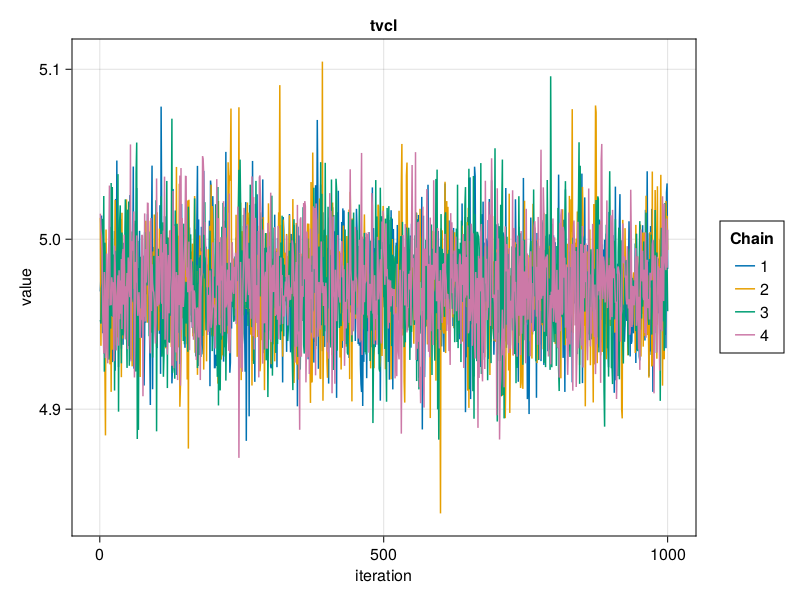
\includegraphics[width=1\textwidth]{trace_1.png}
        \end{column}
        \begin{column}{0.5\textwidth}
            The trace plot of a parameter shows the value of the parameter in each iteration of the MCMC algorithm.
        \end{column}
    \end{columns}
\end{frame}

\begin{frame}{Trace Plot}
    \begin{columns}
        \begin{column}{0.5\textwidth}
            \centering
            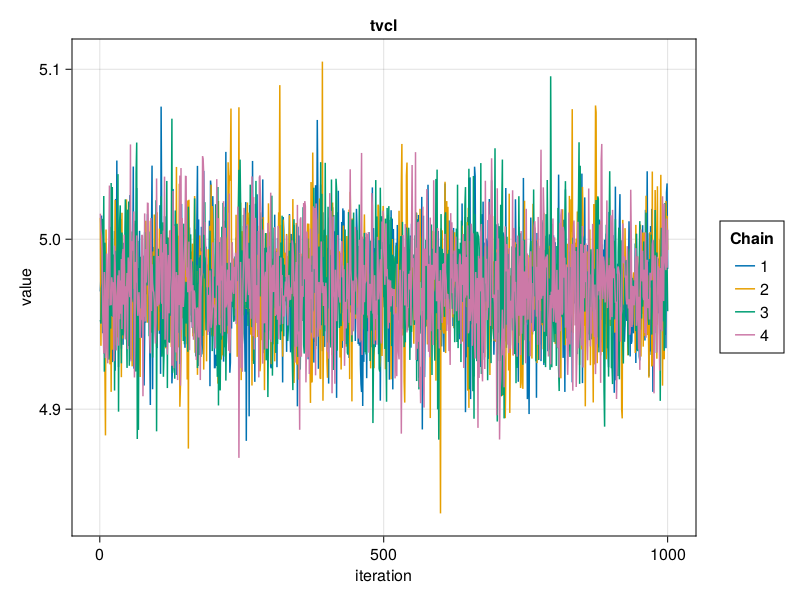
\includegraphics[width=1\textwidth]{trace_1.png}
        \end{column}
        \begin{column}{0.5\textwidth}
            A good trace plot is one that:
            \vfill
            \begin{vfilleditems}
                \item Is noisy, not an increasing or decreasing line for example.
                \item Has a fixed mean.
                \item Has a fixed variance.
                \item Shows all chains overlapping with each other, aka chain mixing.
            \end{vfilleditems}
            \vfill
            This is an example of somewhat well mixed chains that don't indicate non-convergence.
        \end{column}
    \end{columns}
\end{frame}

\begin{frame}{Cumulative Mean Plot}
    \begin{columns}
        \begin{column}{0.5\textwidth}
            \centering
            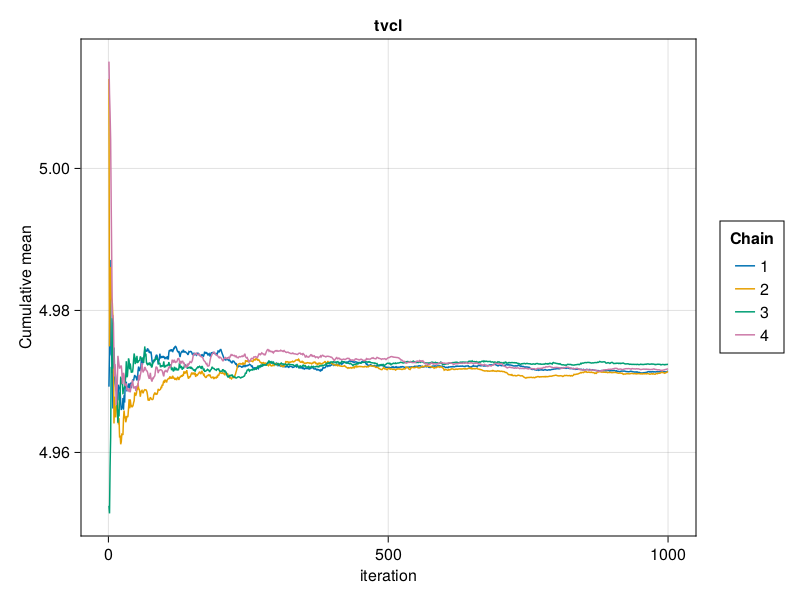
\includegraphics[width=1\textwidth]{cummean_1.png}
        \end{column}
        \begin{column}{0.5\textwidth}
            The cumulative mean plot of a parameter shows the mean of the parameter value in each MCMC chain up to a certain iteration.
        \end{column}
    \end{columns}
\end{frame}

\begin{frame}{Cumulative Mean Plot}
    \begin{columns}
        \begin{column}{0.5\textwidth}
            \centering
            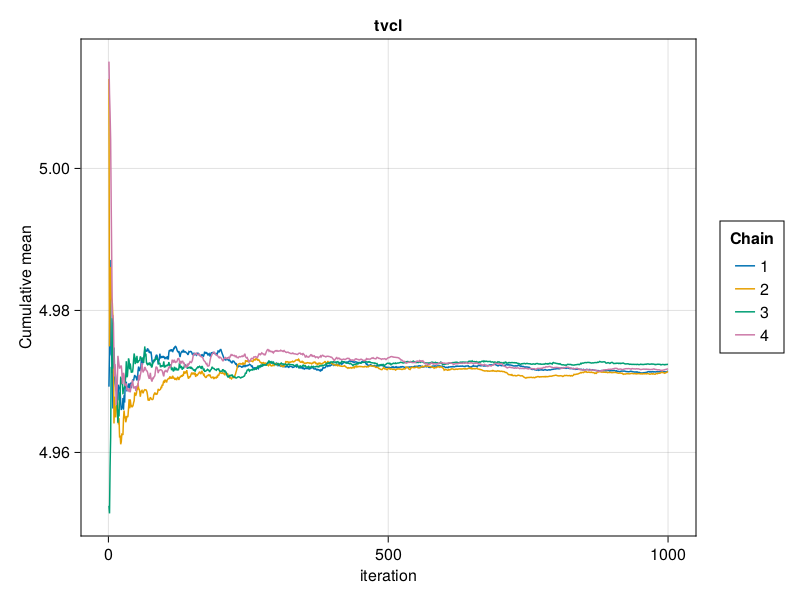
\includegraphics[width=1\textwidth]{cummean_1.png}
        \end{column}
        \begin{column}{0.5\textwidth}
            An MCMC chain converging to a stationary posterior distribution should have the cumulative mean of each parameter converge to a fixed value.
        \end{column}
    \end{columns}
\end{frame}

\begin{frame}{Cumulative Mean Plot}
    \begin{columns}
        \begin{column}{0.5\textwidth}
            \centering
            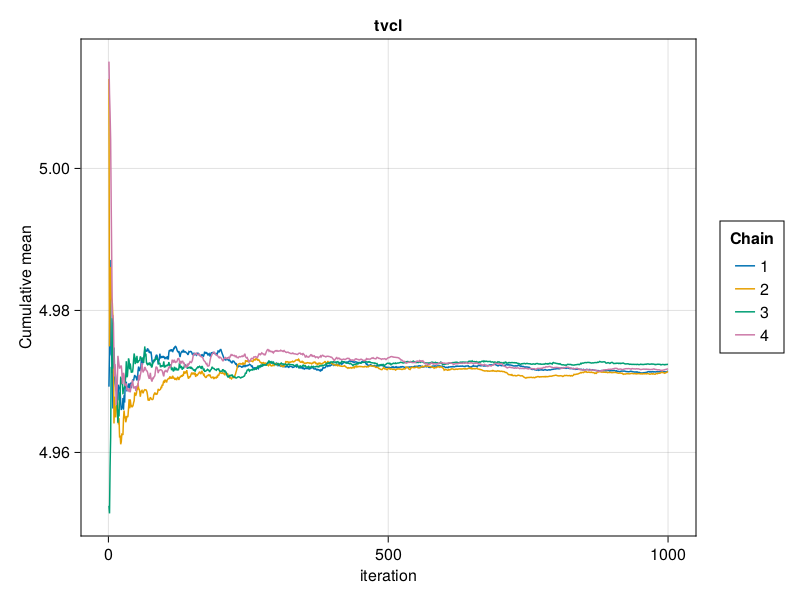
\includegraphics[width=1\textwidth]{cummean_1.png}
        \end{column}
        \begin{column}{0.5\textwidth}
            All the chains should be converging to the same mean for a given parameter, the posterior mean.
        \end{column}
    \end{columns}
\end{frame}

\begin{frame}{Density Plot}
    \begin{columns}
        \begin{column}{0.5\textwidth}
            \centering
            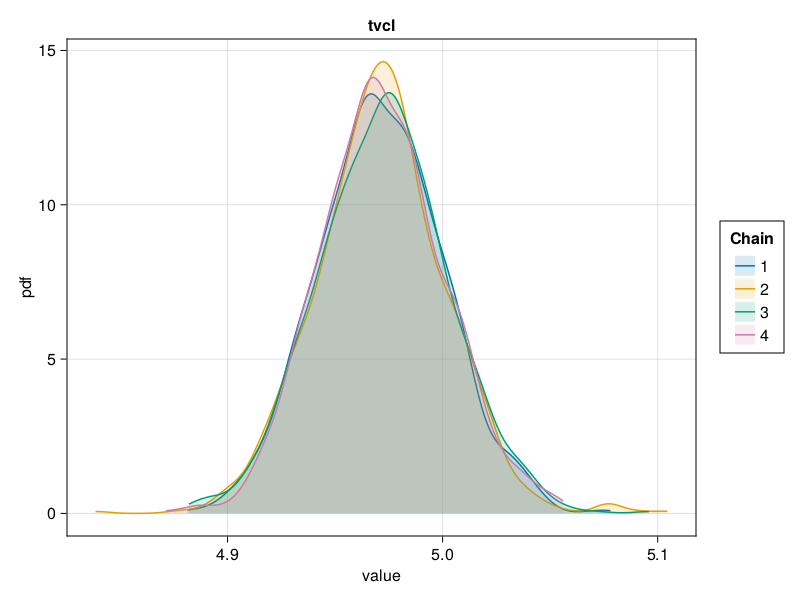
\includegraphics[width=1\textwidth]{density_1.png}
        \end{column}
        \begin{column}{0.5\textwidth}
            \begin{vfilleditems}
                \item The density plot of a parameter shows a smoothed version of the histogram of the parameter values, giving an approximate probability density function for the marginal posterior of the parameter considered.
                \item This helps us visualize the shape of the marginal posterior of each parameter.
            \end{vfilleditems}
        \end{column}
    \end{columns}
\end{frame}

\begin{frame}{Auto-correlation Plot}
    \begin{columns}
        \begin{column}{0.5\textwidth}
            \centering
            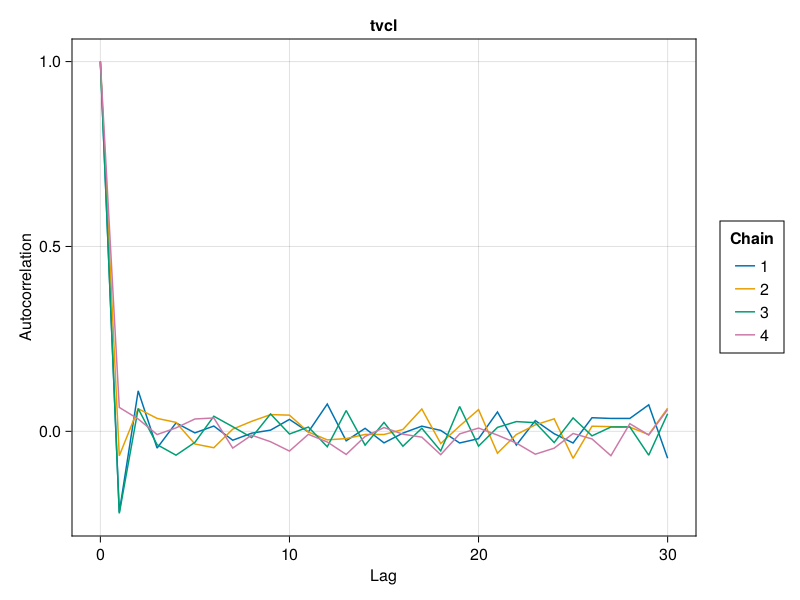
\includegraphics[width=1\textwidth]{corplot_1.png}
        \end{column}
        \begin{column}{0.5\textwidth}
            \begin{vfilleditems}
                \item MCMC chains are prone to auto-correlation between the samples because each sample in the chain is a function of the previous sample.
                \item The auto-correlation plot shows the correlation between every sample with index $s$ and the corresponding sample with index $s + \text{lag}$ for all $s \in 1:N-\text{lag}$ where $N$ is the total number of samples.
            \end{vfilleditems}
        \end{column}
    \end{columns}
\end{frame}

\begin{frame}{Auto-correlation Plot}
    \begin{columns}
        \begin{column}{0.5\textwidth}
            \centering
            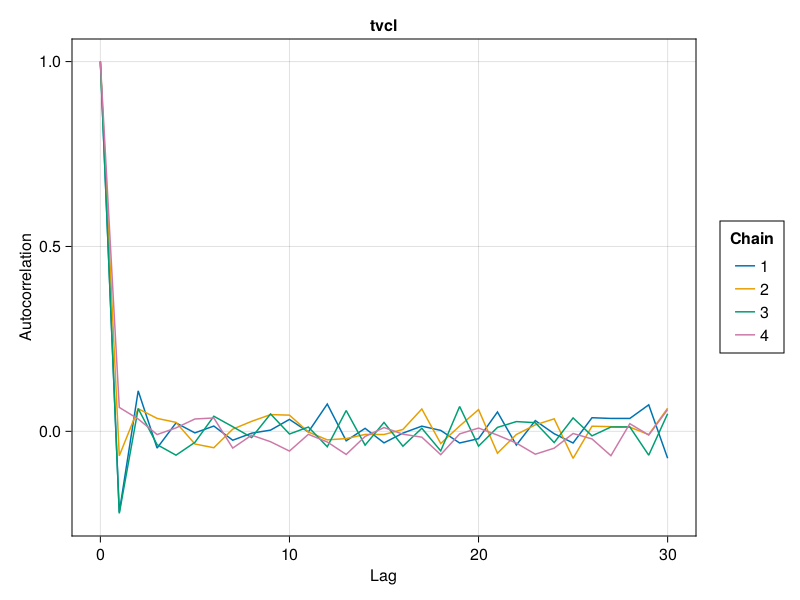
\includegraphics[width=1\textwidth]{corplot_1.png}
        \end{column}
        \begin{column}{0.5\textwidth}
            \begin{vfilleditems}
                \item For each value of $\text{lag}$, we can compute a correlation measure between the samples and their $\text{lag}$-steps-ahead counterparts.
                \item The correlation is usually a value between 0 and 1 but can sometimes be between -1 and 0 as well.
            \end{vfilleditems}
        \end{column}
    \end{columns}
\end{frame}

\begin{frame}{Auto-correlation Plot}
    \begin{columns}
        \begin{column}{0.5\textwidth}
            \centering
            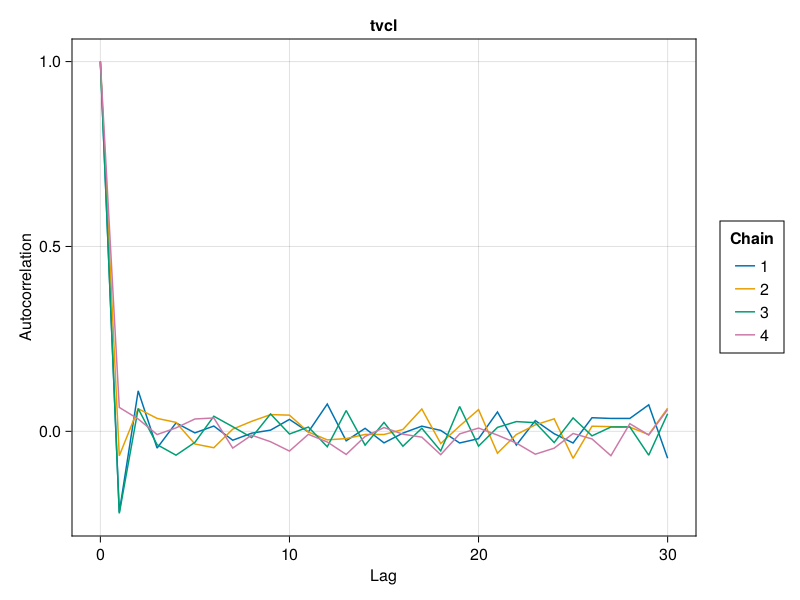
\includegraphics[width=1\textwidth]{corplot_1.png}
        \end{column}
        \begin{column}{0.5\textwidth}
            \begin{vfilleditems}
                \item The auto-correlation plot shows the $\text{lag}$ on the x-axis and the correlation value on the y-axis.
                \item For well behaving MCMC chains when $\text{lag}$ increases, the corresponding correlation gets closer to 0.
            \end{vfilleditems}
        \end{column}
    \end{columns}
\end{frame}

\begin{frame}{Auto-correlation Plot}
    \begin{columns}
        \begin{column}{0.5\textwidth}
            \centering
            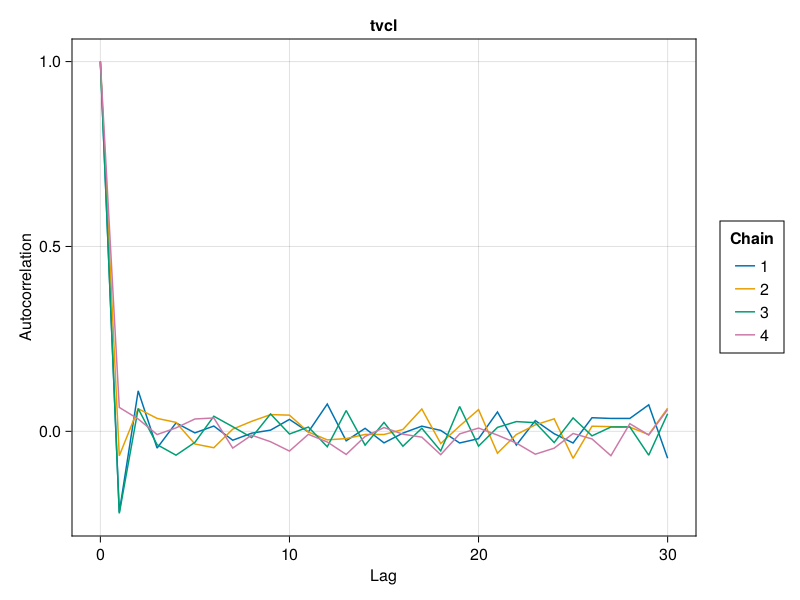
\includegraphics[width=1\textwidth]{corplot_1.png}
        \end{column}
        \begin{column}{0.5\textwidth}
            \begin{vfilleditems}
                \item This means that there is less and less correlation between any 2 samples further away from each other.
                \item The value of $\text{lag}$ where the correlation becomes close to 0 can be used to guide the thinning of the MCMC samples to extract mostly independent samples from the auto-correlated samples.
            \end{vfilleditems}
        \end{column}
    \end{columns}
\end{frame}

\begin{frame}{Ridge Line Plot}
    \begin{columns}
        \begin{column}{0.5\textwidth}
            \centering
            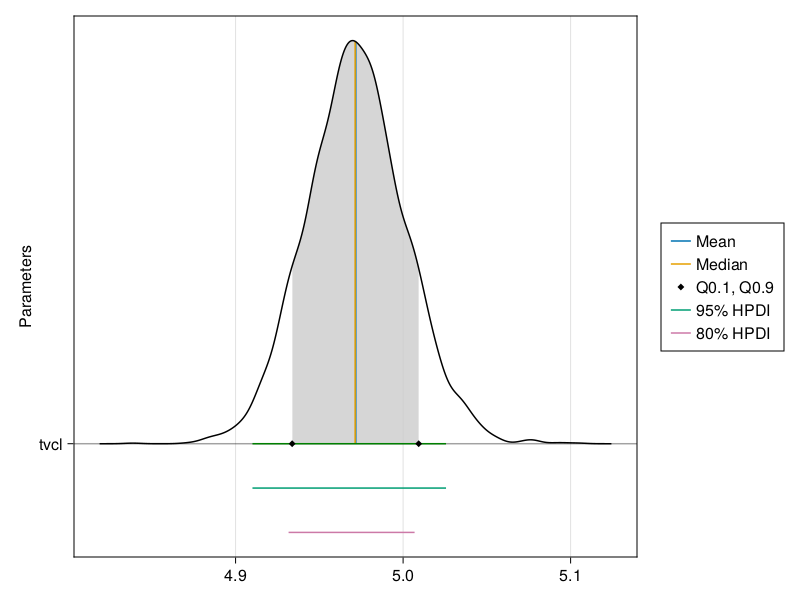
\includegraphics[width=1\textwidth]{ridge_1.png}
        \end{column}
        \begin{column}{0.5\textwidth}
            The ridge line plot shows similar information as the density plot in addition to the credible interval and quantile information.
        \end{column}
    \end{columns}
\end{frame}

\begin{frame}{Corner Plot}
    \centering
    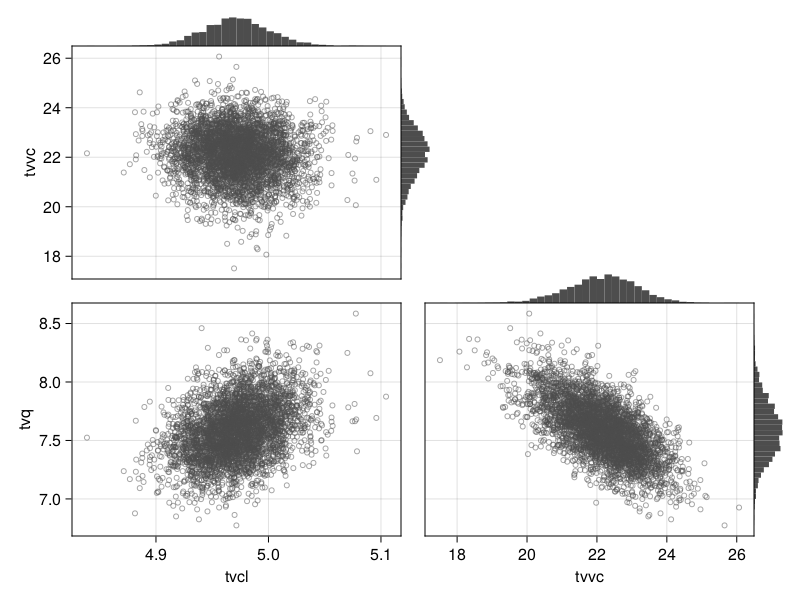
\includegraphics[width=0.6\textwidth]{corner_1.png}
\end{frame}

\subsection{Other Diagnostics}
\begin{frame}{Convergence Metrics}
    There are a few metrics and diagnostics usually used to assess and diagnose the Markov chains:
    \begin{vfilleditems}
        \item \textbf{Effective Sample Size} (ESS):
        an approximation of the ``number of independent samples'' generated by a Markov chain.
        \item $\widehat{R}$ (\textbf{Rhat}):
        potential scale reduction factor,
        a metric to measure if the Markov chain have mixed,
        and, potentially, converged.
    \end{vfilleditems}
\end{frame}

\begin{frame}{Effective Sample Size \parencite{gelman2013bayesian}}
    $$\widehat{n}_{\text{eff}} = \frac{mn}{1 + \sum_{t=1}^T \widehat{\rho}_t}$$
    Where:
    \begin{vfilleditems}
        \item $m$: number of Markov chains.
        \item $n$: total samples per Markov chain (discarding warmup).
        \item $\widehat{\rho}_t$: an autocorrelation estimate.
    \end{vfilleditems}
\end{frame}

\begin{frame}{Rhat \parencite{gelman2013bayesian}}
    $$\widehat{R} = \sqrt{\frac{\widehat{\text{var}}^+(\psi \mid y)}{W}}$$
    where $\widehat{\text{var}}^+(\psi \mid y)$ is the Markov chains' sample variance
    for a certain parameter $\psi$.
    We calculate it by using a weighted sum of the within-chain $W$
    and between-chain $B$ variances:
    $$\widehat{\text{var}}^+(\psi \mid y) = \frac{n-1}{n} W + \frac{1}{n} B$$
    \vfill
    Intuitively, the value is $1.0$ if all chains are totally convergent.
    As a heuristic, if $\widehat{R} > 1.1$,
    you need to worry because probably the chains have not converged adequate.
\end{frame}

% % plots taken from script:
% % slides/images/bad_chains_traceplot.tex
% \begin{frame}{Traceplot -- Convergent Markov Chains}
%     \begin{figure}
%         \centering
%         \resizebox{.4\linewidth}{!}{% Created by tikzDevice version 0.12.3.1 on 2021-05-31 11:59:55
% !TEX encoding = UTF-8 Unicode
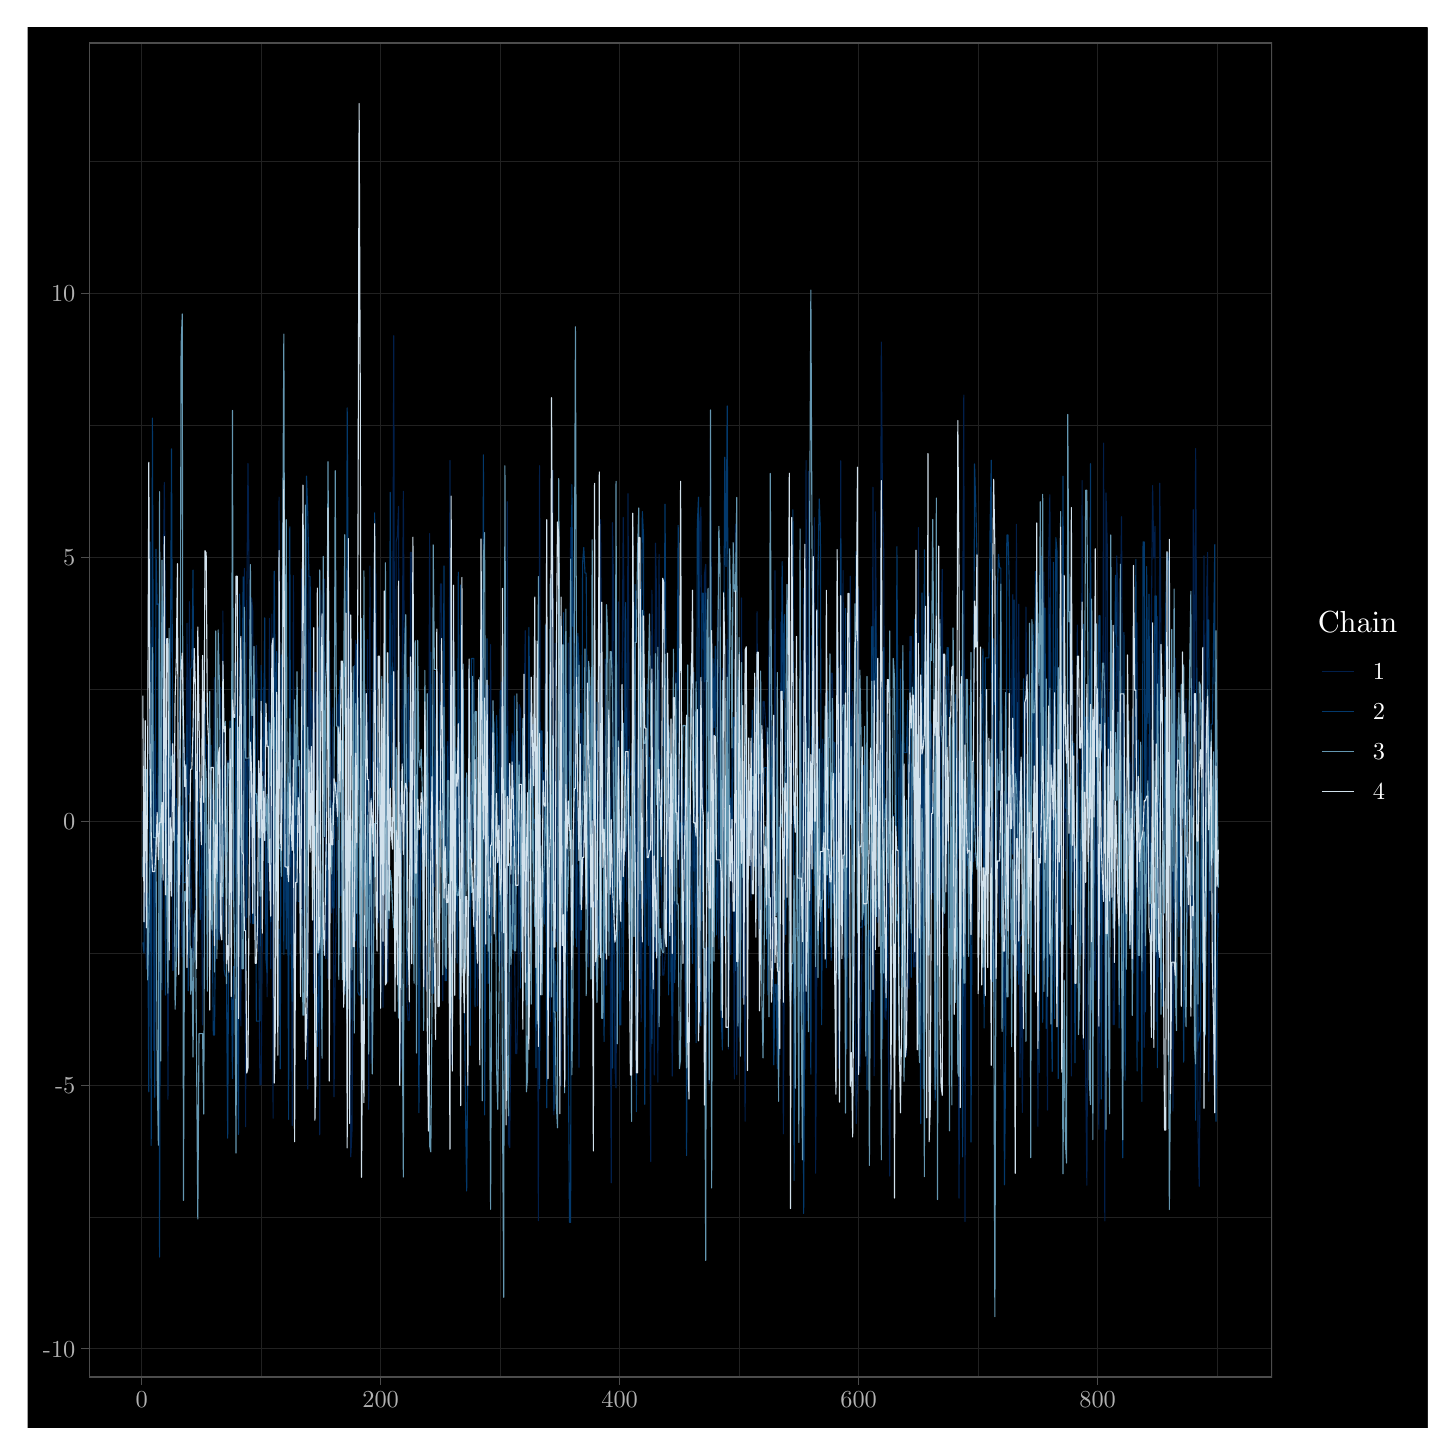
\begin{tikzpicture}[x=1pt,y=1pt]
\definecolor{fillColor}{RGB}{255,255,255}
\path[use as bounding box,fill=fillColor,fill opacity=0.00] (0,0) rectangle (505.89,505.89);
\begin{scope}
\path[clip] (  0.00,  0.00) rectangle (505.89,505.89);
\definecolor{drawColor}{RGB}{0,0,0}
\definecolor{fillColor}{RGB}{0,0,0}

\path[draw=drawColor,line width= 0.6pt,line join=round,line cap=round,fill=fillColor] (  0.00,  0.00) rectangle (505.89,505.89);
\end{scope}
\begin{scope}
\path[clip] ( 22.18, 18.22) rectangle (449.67,500.39);
\definecolor{fillColor}{RGB}{0,0,0}

\path[fill=fillColor] ( 22.18, 18.22) rectangle (449.67,500.39);
\definecolor{drawColor}{gray}{0.13}

\path[draw=drawColor,line width= 0.1pt,line join=round] ( 22.18, 76.16) --
	(449.67, 76.16);

\path[draw=drawColor,line width= 0.1pt,line join=round] ( 22.18,171.51) --
	(449.67,171.51);

\path[draw=drawColor,line width= 0.1pt,line join=round] ( 22.18,266.86) --
	(449.67,266.86);

\path[draw=drawColor,line width= 0.1pt,line join=round] ( 22.18,362.20) --
	(449.67,362.20);

\path[draw=drawColor,line width= 0.1pt,line join=round] ( 22.18,457.55) --
	(449.67,457.55);

\path[draw=drawColor,line width= 0.1pt,line join=round] ( 84.36, 18.22) --
	( 84.36,500.39);

\path[draw=drawColor,line width= 0.1pt,line join=round] (170.72, 18.22) --
	(170.72,500.39);

\path[draw=drawColor,line width= 0.1pt,line join=round] (257.09, 18.22) --
	(257.09,500.39);

\path[draw=drawColor,line width= 0.1pt,line join=round] (343.45, 18.22) --
	(343.45,500.39);

\path[draw=drawColor,line width= 0.1pt,line join=round] (429.81, 18.22) --
	(429.81,500.39);

\path[draw=drawColor,line width= 0.3pt,line join=round] ( 22.18, 28.49) --
	(449.67, 28.49);

\path[draw=drawColor,line width= 0.3pt,line join=round] ( 22.18,123.84) --
	(449.67,123.84);

\path[draw=drawColor,line width= 0.3pt,line join=round] ( 22.18,219.18) --
	(449.67,219.18);

\path[draw=drawColor,line width= 0.3pt,line join=round] ( 22.18,314.53) --
	(449.67,314.53);

\path[draw=drawColor,line width= 0.3pt,line join=round] ( 22.18,409.88) --
	(449.67,409.88);

\path[draw=drawColor,line width= 0.3pt,line join=round] ( 41.18, 18.22) --
	( 41.18,500.39);

\path[draw=drawColor,line width= 0.3pt,line join=round] (127.54, 18.22) --
	(127.54,500.39);

\path[draw=drawColor,line width= 0.3pt,line join=round] (213.91, 18.22) --
	(213.91,500.39);

\path[draw=drawColor,line width= 0.3pt,line join=round] (300.27, 18.22) --
	(300.27,500.39);

\path[draw=drawColor,line width= 0.3pt,line join=round] (386.63, 18.22) --
	(386.63,500.39);
\definecolor{drawColor}{RGB}{1,31,75}

\path[draw=drawColor,line width= 0.4pt,line join=round] ( 41.61,222.92) --
	( 42.04,204.96) --
	( 42.48,206.25) --
	( 42.91,165.69) --
	( 43.34,165.69) --
	( 43.77,163.58) --
	( 44.20,221.08) --
	( 44.63,210.00) --
	( 45.07,275.91) --
	( 45.50,136.32) --
	( 45.93,248.08) --
	( 46.36,228.21) --
	( 46.79,218.61) --
	( 47.23,245.67) --
	( 47.66,213.48) --
	( 48.09,255.03) --
	( 48.52,158.23) --
	( 48.95,299.50) --
	( 49.38,341.55) --
	( 49.82,283.34) --
	( 50.25,283.34) --
	( 50.68,118.63) --
	( 51.11,204.07) --
	( 51.54,217.46) --
	( 51.98,247.07) --
	( 52.41,165.21) --
	( 52.84,165.58) --
	( 53.27,244.06) --
	( 53.70,170.69) --
	( 54.13,217.63) --
	( 54.57,225.28) --
	( 55.00,221.31) --
	( 55.43,189.70) --
	( 55.86,170.14) --
	( 56.29,251.82) --
	( 56.73,241.96) --
	( 57.16,197.19) --
	( 57.59,290.64) --
	( 58.02,228.73) --
	( 58.45,298.48) --
	( 58.88,202.02) --
	( 59.32,187.21) --
	( 59.75,167.25) --
	( 60.18,185.49) --
	( 60.61,185.49) --
	( 61.04,209.39) --
	( 61.48,249.73) --
	( 61.91,229.47) --
	( 62.34,229.47) --
	( 62.77,207.24) --
	( 63.20,145.54) --
	( 63.63,251.30) --
	( 64.07,246.69) --
	( 64.50,246.69) --
	( 64.93,246.69) --
	( 65.36,226.98) --
	( 65.79,158.71) --
	( 66.23,226.74) --
	( 66.66,228.86) --
	( 67.09,219.07) --
	( 67.52,271.03) --
	( 67.95,236.38) --
	( 68.38,247.12) --
	( 68.82,207.82) --
	( 69.25,176.18) --
	( 69.68,267.48) --
	( 70.11,179.57) --
	( 70.54,295.11) --
	( 70.98,205.16) --
	( 71.41,231.62) --
	( 71.84,231.62) --
	( 72.27,240.95) --
	( 72.70,240.95) --
	( 73.13,196.06) --
	( 73.57,190.89) --
	( 74.00,190.89) --
	( 74.43,227.82) --
	( 74.86,203.44) --
	( 75.29,203.44) --
	( 75.73,259.20) --
	( 76.16,134.68) --
	( 76.59,265.00) --
	( 77.02,145.18) --
	( 77.45,265.84) --
	( 77.88,168.13) --
	( 78.32,310.48) --
	( 78.75,108.72) --
	( 79.18,298.87) --
	( 79.61,348.38) --
	( 80.04,302.02) --
	( 80.48,182.41) --
	( 80.91,299.84) --
	( 81.34,294.94) --
	( 81.77,200.94) --
	( 82.20,261.79) --
	( 82.63,282.66) --
	( 83.07,258.84) --
	( 83.50,174.13) --
	( 83.93,123.91) --
	( 84.36,123.91) --
	( 84.79,177.59) --
	( 85.23,267.42) --
	( 85.66,225.41) --
	( 86.09,225.87) --
	( 86.52,155.73) --
	( 86.95,223.15) --
	( 87.38,292.38) --
	( 87.82,165.90) --
	( 88.25,293.99) --
	( 88.68,111.82) --
	( 89.11,308.27) --
	( 89.54,192.52) --
	( 89.98,216.75) --
	( 90.41,233.78) --
	( 90.84,336.24) --
	( 91.27,257.34) --
	( 91.70,223.61) --
	( 92.13,237.18) --
	( 92.57,195.07) --
	( 93.00,189.85) --
	( 93.43,223.60) --
	( 93.86,198.09) --
	( 94.29,199.33) --
	( 94.72,254.04) --
	( 95.16,254.04) --
	( 95.59,109.19) --
	( 96.02,307.88) --
	( 96.45,144.58) --
	( 96.88,176.90) --
	( 97.32,267.32) --
	( 97.75,209.88) --
	( 98.18,230.93) --
	( 98.61,159.53) --
	( 99.04,310.33) --
	( 99.47,164.82) --
	( 99.91,264.89) --
	(100.34,261.06) --
	(100.77,326.53) --
	(101.20,122.36) --
	(101.63,308.11) --
	(102.07,212.60) --
	(102.50,266.07) --
	(102.93,260.38) --
	(103.36,156.96) --
	(103.79,272.85) --
	(104.22,272.85) --
	(104.66,176.68) --
	(105.09,289.38) --
	(105.52,105.81) --
	(105.95,302.47) --
	(106.38,272.05) --
	(106.82,306.64) --
	(107.25,306.64) --
	(107.68,169.46) --
	(108.11,196.34) --
	(108.54,162.32) --
	(108.97,283.98) --
	(109.41,252.06) --
	(109.84,185.97) --
	(110.27,260.11) --
	(110.70,119.57) --
	(111.13,165.42) --
	(111.57,190.26) --
	(112.00,260.97) --
	(112.43,264.92) --
	(112.86,192.31) --
	(113.29,192.31) --
	(113.72,251.86) --
	(114.16,212.46) --
	(114.59,210.38) --
	(115.02,236.67) --
	(115.45,253.40) --
	(115.88,268.63) --
	(116.32,294.83) --
	(116.75, 97.84) --
	(117.18,107.08) --
	(117.61,183.53) --
	(118.04,250.33) --
	(118.47,284.46) --
	(118.91,207.24) --
	(119.34,287.32) --
	(119.77,276.65) --
	(120.20,169.57) --
	(120.63,158.92) --
	(121.07,188.43) --
	(121.50,215.85) --
	(121.93,266.11) --
	(122.36,155.30) --
	(122.79,284.70) --
	(123.22,115.02) --
	(123.66,311.31) --
	(124.09,131.66) --
	(124.52,146.35) --
	(124.95,288.28) --
	(125.38,291.99) --
	(125.82,308.56) --
	(126.25,210.54) --
	(126.68,182.48) --
	(127.11,230.44) --
	(127.54,206.43) --
	(127.97,209.22) --
	(128.41,151.90) --
	(128.84,270.42) --
	(129.27,172.92) --
	(129.70,269.16) --
	(130.13,161.18) --
	(130.57,219.84) --
	(131.00,267.06) --
	(131.43,267.06) --
	(131.86,267.06) --
	(132.29,394.56) --
	(132.72,162.09) --
	(133.16,320.31) --
	(133.59,322.13) --
	(134.02,332.88) --
	(134.45,127.98) --
	(134.88,130.69) --
	(135.32,272.58) --
	(135.75,338.32) --
	(136.18,259.09) --
	(136.61,212.76) --
	(137.04,154.32) --
	(137.47,147.11) --
	(137.91,147.11) --
	(138.34,316.23) --
	(138.77,316.23) --
	(139.20,174.68) --
	(139.63,275.28) --
	(140.07,245.70) --
	(140.50,225.62) --
	(140.93,225.62) --
	(141.36,160.81) --
	(141.79,211.09) --
	(142.22,201.63) --
	(142.66,201.63) --
	(143.09,203.07) --
	(143.52,160.90) --
	(143.95,158.15) --
	(144.38,240.01) --
	(144.82,208.37) --
	(145.25,323.11) --
	(145.68,218.63) --
	(146.11,228.25) --
	(146.54,235.61) --
	(146.97,195.45) --
	(147.41,241.57) --
	(147.84,238.44) --
	(148.27,194.05) --
	(148.70,238.79) --
	(149.13,304.87) --
	(149.57,304.87) --
	(150.00,154.25) --
	(150.43,295.19) --
	(150.86,214.66) --
	(151.29,185.17) --
	(151.72,247.93) --
	(152.16,204.36) --
	(152.59,349.52) --
	(153.02,131.11) --
	(153.45,247.59) --
	(153.88,298.77) --
	(154.32,192.19) --
	(154.75,232.17) --
	(155.18,179.93) --
	(155.61,232.53) --
	(156.04,244.37) --
	(156.47,233.66) --
	(156.91,260.53) --
	(157.34,176.14) --
	(157.77,192.72) --
	(158.20,234.69) --
	(158.63,216.74) --
	(159.07,216.74) --
	(159.50,236.61) --
	(159.93,236.61) --
	(160.36,236.61) --
	(160.79,204.45) --
	(161.22,235.53) --
	(161.66,235.53) --
	(162.09,243.95) --
	(162.52,152.44) --
	(162.95,199.80) --
	(163.38,220.79) --
	(163.81,242.29) --
	(164.25,277.88) --
	(164.68,300.31) --
	(165.11,211.07) --
	(165.54,268.21) --
	(165.97,268.21) --
	(166.41,268.21) --
	(166.84,165.59) --
	(167.27,282.95) --
	(167.70,184.84) --
	(168.13,202.35) --
	(168.56,202.35) --
	(169.00,202.35) --
	(169.43,204.21) --
	(169.86,212.66) --
	(170.29,203.46) --
	(170.72,162.25) --
	(171.16,269.40) --
	(171.59,154.24) --
	(172.02,271.32) --
	(172.45,132.51) --
	(172.88,132.51) --
	(173.31,334.59) --
	(173.75,102.61) --
	(174.18,101.20) --
	(174.61,149.64) --
	(175.04,250.80) --
	(175.47,245.24) --
	(175.91,173.38) --
	(176.34,135.21) --
	(176.77,135.21) --
	(177.20,159.79) --
	(177.63,261.28) --
	(178.06,259.53) --
	(178.50,183.64) --
	(178.93,255.55) --
	(179.36,255.55) --
	(179.79,287.98) --
	(180.22,152.39) --
	(180.66,224.90) --
	(181.09,197.18) --
	(181.52,262.95) --
	(181.95,229.53) --
	(182.38,254.11) --
	(182.81,254.11) --
	(183.25,235.41) --
	(183.68,224.39) --
	(184.11,232.92) --
	(184.54, 74.82) --
	(184.97,347.62) --
	(185.41,168.41) --
	(185.84,166.59) --
	(186.27,236.73) --
	(186.70,236.73) --
	(187.13,214.30) --
	(187.56,285.52) --
	(188.00,173.92) --
	(188.43,235.52) --
	(188.86,146.72) --
	(189.29,302.12) --
	(189.72,345.93) --
	(190.16,113.05) --
	(190.59,283.45) --
	(191.02,175.61) --
	(191.45,233.57) --
	(191.88,263.54) --
	(192.31,273.09) --
	(192.75,123.35) --
	(193.18,277.14) --
	(193.61,152.00) --
	(194.04,261.74) --
	(194.47,238.10) --
	(194.91,178.76) --
	(195.34,283.52) --
	(195.77,230.76) --
	(196.20,325.23) --
	(196.63,325.23) --
	(197.06,298.16) --
	(197.50,275.75) --
	(197.93,176.93) --
	(198.36,203.33) --
	(198.79,203.33) --
	(199.22,130.22) --
	(199.66,257.99) --
	(200.09,257.99) --
	(200.52,190.68) --
	(200.95,215.00) --
	(201.38,255.58) --
	(201.81,226.40) --
	(202.25,209.04) --
	(202.68,166.48) --
	(203.11,226.76) --
	(203.54,234.61) --
	(203.97,170.36) --
	(204.41,271.08) --
	(204.84,271.08) --
	(205.27,166.11) --
	(205.70,154.54) --
	(206.13,228.03) --
	(206.56,228.03) --
	(207.00,328.11) --
	(207.43,267.36) --
	(207.86,248.84) --
	(208.29,159.32) --
	(208.72,277.74) --
	(209.16,159.95) --
	(209.59,259.92) --
	(210.02,251.69) --
	(210.45,176.92) --
	(210.88, 88.49) --
	(211.31,326.99) --
	(211.75,302.15) --
	(212.18,130.73) --
	(212.61,122.77) --
	(213.04,231.55) --
	(213.47,298.38) --
	(213.91,208.92) --
	(214.34,183.21) --
	(214.77,266.11) --
	(215.20,328.92) --
	(215.63,275.58) --
	(216.06,228.15) --
	(216.50,190.04) --
	(216.93,337.48) --
	(217.36,237.22) --
	(217.79,235.90) --
	(218.22,235.90) --
	(218.66,250.22) --
	(219.09,195.27) --
	(219.52,269.65) --
	(219.95,234.71) --
	(220.38,135.94) --
	(220.81,216.79) --
	(221.25,216.79) --
	(221.68,146.71) --
	(222.11,187.27) --
	(222.54,190.58) --
	(222.97,199.96) --
	(223.41,191.56) --
	(223.84,190.99) --
	(224.27,259.67) --
	(224.70,168.18) --
	(225.13, 96.15) --
	(225.56,302.60) --
	(226.00,267.27) --
	(226.43,127.44) --
	(226.86,319.59) --
	(227.29,298.08) --
	(227.72,124.84) --
	(228.15,315.52) --
	(228.59,215.33) --
	(229.02,200.82) --
	(229.45,163.51) --
	(229.88,163.51) --
	(230.31,169.58) --
	(230.75,221.82) --
	(231.18,182.37) --
	(231.61,255.83) --
	(232.04,201.28) --
	(232.47,190.94) --
	(232.90,127.05) --
	(233.34,164.62) --
	(233.77,204.86) --
	(234.20,272.92) --
	(234.63,213.36) --
	(235.06,234.81) --
	(235.50,195.33) --
	(235.93,241.61) --
	(236.36,241.61) --
	(236.79,199.72) --
	(237.22,230.39) --
	(237.65,137.58) --
	(238.09,210.85) --
	(238.52,213.95) --
	(238.95,229.59) --
	(239.38,229.59) --
	(239.81,216.47) --
	(240.25,213.41) --
	(240.68,201.11) --
	(241.11,201.11) --
	(241.54,231.57) --
	(241.97,251.95) --
	(242.40,222.13) --
	(242.84,327.31) --
	(243.27,332.60) --
	(243.70,231.15) --
	(244.13,214.30) --
	(244.56,308.26) --
	(245.00,311.94) --
	(245.43,150.45) --
	(245.86,173.45) --
	(246.29,124.31) --
	(246.72,357.41) --
	(247.15,285.56) --
	(247.59,268.10) --
	(248.02,207.97) --
	(248.45,246.58) --
	(248.88,266.35) --
	(249.31,295.27) --
	(249.75,172.91) --
	(250.18,299.37) --
	(250.61,149.03) --
	(251.04,274.35) --
	(251.47,208.32) --
	(251.90,228.02) --
	(252.34,184.53) --
	(252.77,284.84) --
	(253.20,136.83) --
	(253.63,191.44) --
	(254.06,171.04) --
	(254.50,245.65) --
	(254.93,206.81) --
	(255.36,125.98) --
	(255.79,326.46) --
	(256.22,127.62) --
	(256.65,179.01) --
	(257.09,141.07) --
	(257.52,156.26) --
	(257.95,299.85) --
	(258.38,155.33) --
	(258.81,190.77) --
	(259.25,110.71) --
	(259.68,231.06) --
	(260.11,202.37) --
	(260.54,227.10) --
	(260.97,230.19) --
	(261.40,190.56) --
	(261.84,249.98) --
	(262.27,208.94) --
	(262.70,261.17) --
	(263.13,202.73) --
	(263.56,294.85) --
	(264.00,191.59) --
	(264.43,251.84) --
	(264.86,251.84) --
	(265.29,179.27) --
	(265.72,262.38) --
	(266.15,262.38) --
	(266.59,255.59) --
	(267.02,249.27) --
	(267.45,222.41) --
	(267.88,291.33) --
	(268.31,292.64) --
	(268.75,164.48) --
	(269.18,253.44) --
	(269.61,165.61) --
	(270.04,309.71) --
	(270.47,208.44) --
	(270.90,245.62) --
	(271.34,163.88) --
	(271.77,134.74) --
	(272.20,291.18) --
	(272.63,291.18) --
	(273.06,106.19) --
	(273.50,186.97) --
	(273.93,186.97) --
	(274.36,278.80) --
	(274.79,231.40) --
	(275.22,231.40) --
	(275.65,232.42) --
	(276.09,240.48) --
	(276.52,241.07) --
	(276.95,217.04) --
	(277.38,221.04) --
	(277.81,221.04) --
	(278.25,201.56) --
	(278.68,201.56) --
	(279.11,148.95) --
	(279.54,277.11) --
	(279.97,150.00) --
	(280.40,303.33) --
	(280.84,129.74) --
	(281.27,349.46) --
	(281.70,147.02) --
	(282.13,345.55) --
	(282.56,176.98) --
	(283.00,188.20) --
	(283.43,251.89) --
	(283.86,251.89) --
	(284.29,328.82) --
	(284.72, 91.94) --
	(285.15,166.38) --
	(285.59,253.28) --
	(286.02,215.18) --
	(286.45,181.22) --
	(286.88,173.32) --
	(287.31,248.83) --
	(287.75,197.16) --
	(288.18,197.16) --
	(288.61,196.87) --
	(289.04,254.67) --
	(289.47,206.59) --
	(289.90,202.92) --
	(290.34,272.60) --
	(290.77,272.60) --
	(291.20,249.27) --
	(291.63,226.12) --
	(292.06,165.31) --
	(292.49,288.85) --
	(292.93,129.91) --
	(293.36,130.14) --
	(293.79,349.38) --
	(294.22,192.39) --
	(294.65,309.69) --
	(295.09,165.65) --
	(295.52,228.50) --
	(295.95,223.66) --
	(296.38,169.82) --
	(296.81,226.73) --
	(297.24,307.66) --
	(297.68,217.37) --
	(298.11,265.96) --
	(298.54,206.11) --
	(298.97,151.02) --
	(299.40,109.85) --
	(299.84,123.71) --
	(300.27,303.13) --
	(300.70,128.47) --
	(301.13,150.23) --
	(301.56,176.60) --
	(301.99,193.33) --
	(302.43,231.98) --
	(302.86,245.01) --
	(303.29,216.83) --
	(303.72,222.26) --
	(304.15,222.26) --
	(304.59,198.91) --
	(305.02,153.94) --
	(305.45,339.80) --
	(305.88,127.20) --
	(306.31,330.91) --
	(306.74,281.91) --
	(307.18,182.56) --
	(307.61,184.79) --
	(308.04,253.58) --
	(308.47,392.28) --
	(308.90,331.12) --
	(309.34,317.02) --
	(309.77,148.46) --
	(310.20,147.44) --
	(310.63,269.75) --
	(311.06,135.06) --
	(311.49, 90.91) --
	(311.93,156.05) --
	(312.36,197.55) --
	(312.79,221.32) --
	(313.22,221.32) --
	(313.65,221.32) --
	(314.09,195.69) --
	(314.52,195.69) --
	(314.95,195.69) --
	(315.38,242.20) --
	(315.81,229.43) --
	(316.24,255.22) --
	(316.68,181.19) --
	(317.11,167.40) --
	(317.54,134.34) --
	(317.97,189.22) --
	(318.40,158.51) --
	(318.84,285.93) --
	(319.27,285.93) --
	(319.70,258.19) --
	(320.13,166.52) --
	(320.56,166.52) --
	(320.99,180.45) --
	(321.43,143.65) --
	(321.86,325.23) --
	(322.29,133.99) --
	(322.72,259.48) --
	(323.15,256.00) --
	(323.59,225.65) --
	(324.02,236.00) --
	(324.45,190.69) --
	(324.88,183.95) --
	(325.31,183.95) --
	(325.74,301.59) --
	(326.18,192.65) --
	(326.61,254.26) --
	(327.04,193.38) --
	(327.47,193.38) --
	(327.90,193.38) --
	(328.34,298.42) --
	(328.77,175.38) --
	(329.20,229.10) --
	(329.63,166.47) --
	(330.06,289.73) --
	(330.49,310.16) --
	(330.93,180.70) --
	(331.36,271.44) --
	(331.79,271.44) --
	(332.22,271.44) --
	(332.65,176.35) --
	(333.09,199.79) --
	(333.52,190.79) --
	(333.95,160.47) --
	(334.38,178.70) --
	(334.81,235.40) --
	(335.24,235.40) --
	(335.68,259.46) --
	(336.11,194.78) --
	(336.54, 82.93) --
	(336.97,169.26) --
	(337.40,169.26) --
	(337.84,285.08) --
	(338.27,373.12) --
	(338.70, 74.48) --
	(339.13,224.20) --
	(339.56,205.27) --
	(339.99,235.04) --
	(340.43,183.83) --
	(340.86,269.12) --
	(341.29,204.64) --
	(341.72,204.64) --
	(342.15,207.61) --
	(342.59,207.61) --
	(343.02,233.97) --
	(343.45,211.41) --
	(343.88,178.97) --
	(344.31,229.10) --
	(344.74,209.40) --
	(345.18,230.53) --
	(345.61,177.00) --
	(346.04,177.00) --
	(346.47,208.45) --
	(346.90,232.31) --
	(347.34,232.31) --
	(347.77,218.24) --
	(348.20,178.46) --
	(348.63,210.78) --
	(349.06,223.38) --
	(349.49,148.16) --
	(349.93,187.60) --
	(350.36,304.81) --
	(350.79,202.83) --
	(351.22,178.83) --
	(351.65,282.48) --
	(352.09,259.02) --
	(352.52,227.95) --
	(352.95,145.31) --
	(353.38,182.12) --
	(353.81,237.71) --
	(354.24,211.53) --
	(354.68,225.72) --
	(355.11,176.48) --
	(355.54,257.87) --
	(355.97,301.04) --
	(356.40,171.04) --
	(356.84,157.68) --
	(357.27,326.41) --
	(357.70,165.22) --
	(358.13,297.57) --
	(358.56,126.57) --
	(358.99,171.48) --
	(359.43,113.92) --
	(359.86,185.06) --
	(360.29,195.50) --
	(360.72,296.52) --
	(361.15,253.24) --
	(361.58,247.84) --
	(362.02,247.84) --
	(362.45,247.84) --
	(362.88,254.19) --
	(363.31,268.92) --
	(363.74,163.51) --
	(364.18,269.30) --
	(364.61,278.35) --
	(365.04,108.89) --
	(365.47,271.72) --
	(365.90,187.49) --
	(366.33,253.87) --
	(366.77,259.66) --
	(367.20,309.19) --
	(367.63,221.37) --
	(368.06,215.77) --
	(368.49,114.75) --
	(368.93,314.41) --
	(369.36,337.09) --
	(369.79,256.52) --
	(370.22,182.67) --
	(370.65,267.88) --
	(371.08,186.19) --
	(371.52,222.47) --
	(371.95,187.22) --
	(372.38,256.10) --
	(372.81,253.19) --
	(373.24,218.23) --
	(373.68,273.10) --
	(374.11,237.77) --
	(374.54,237.77) --
	(374.97,201.22) --
	(375.40,228.29) --
	(375.83,243.17) --
	(376.27,257.22) --
	(376.70,306.58) --
	(377.13,127.08) --
	(377.56,277.21) --
	(377.99,186.99) --
	(378.43,208.62) --
	(378.86,193.28) --
	(379.29,290.02) --
	(379.72,193.50) --
	(380.15,187.27) --
	(380.58,187.27) --
	(381.02,342.22) --
	(381.45,136.69) --
	(381.88,264.38) --
	(382.31,126.53) --
	(382.74, 87.61) --
	(383.18,183.91) --
	(383.61,208.55) --
	(384.04,208.55) --
	(384.47,287.98) --
	(384.90,144.45) --
	(385.33,171.96) --
	(385.77,161.68) --
	(386.20,275.67) --
	(386.63,163.13) --
	(387.06,107.84) --
	(387.49,211.34) --
	(387.93,211.34) --
	(388.36,211.34) --
	(388.79,355.75) --
	(389.22, 74.72) --
	(389.65,337.76) --
	(390.08,319.49) --
	(390.52,126.67) --
	(390.95,265.76) --
	(391.38,187.32) --
	(391.81,274.47) --
	(392.24,145.70) --
	(392.68,145.70) --
	(393.11,208.18) --
	(393.54,315.03) --
	(393.97,298.03) --
	(394.40,187.64) --
	(394.83,296.56) --
	(395.27,329.20) --
	(395.70,222.09) --
	(396.13,261.22) --
	(396.56,232.11) --
	(396.99,227.67) --
	(397.43,203.40) --
	(397.86,232.61) --
	(398.29,242.33) --
	(398.72,173.39) --
	(399.15,256.89) --
	(399.58,164.24) --
	(400.02,240.22) --
	(400.45,290.81) --
	(400.88,290.81) --
	(401.31,139.65) --
	(401.74,234.65) --
	(402.18,193.07) --
	(402.61,166.74) --
	(403.04,207.93) --
	(403.47,137.47) --
	(403.90,264.66) --
	(404.33,264.66) --
	(404.77,191.88) --
	(405.20,250.53) --
	(405.63,202.78) --
	(406.06,292.29) --
	(406.49,340.40) --
	(406.93,314.23) --
	(407.36,325.70) --
	(407.79,146.79) --
	(408.22,293.08) --
	(408.65,162.91) --
	(409.08,341.27) --
	(409.52,281.63) --
	(409.95,253.04) --
	(410.38,193.32) --
	(410.81,252.47) --
	(411.24,225.40) --
	(411.68,169.03) --
	(412.11,169.03) --
	(412.54,258.03) --
	(412.97,206.43) --
	(413.40,257.37) --
	(413.83,114.40) --
	(414.27,170.75) --
	(414.70,278.05) --
	(415.13,233.64) --
	(415.56,233.64) --
	(415.99,233.64) --
	(416.43,213.81) --
	(416.86,206.07) --
	(417.29,270.33) --
	(417.72,216.86) --
	(418.15,216.86) --
	(418.58,263.43) --
	(419.02,182.74) --
	(419.45,188.33) --
	(419.88,206.74) --
	(420.31,191.95) --
	(420.74,163.22) --
	(421.18,331.74) --
	(421.61,247.31) --
	(422.04,353.83) --
	(422.47,267.37) --
	(422.90,107.43) --
	(423.33, 87.23) --
	(423.77,140.28) --
	(424.20,244.59) --
	(424.63,174.86) --
	(425.06,314.97) --
	(425.49,141.40) --
	(425.92,297.38) --
	(426.36,316.27) --
	(426.79,125.15) --
	(427.22,229.29) --
	(427.65,231.32) --
	(428.08,217.68) --
	(428.52,127.34) --
	(428.95,218.00) --
	(429.38,276.85) --
	(429.81,181.89) --
	(430.24,185.78);
\definecolor{drawColor}{RGB}{3,57,108}

\path[draw=drawColor,line width= 0.4pt,line join=round] ( 41.61,175.38) --
	( 42.04,171.48) --
	( 42.48,247.21) --
	( 42.91,192.59) --
	( 43.34,193.15) --
	( 43.77,121.36) --
	( 44.20,320.10) --
	( 44.63,102.00) --
	( 45.07,364.80) --
	( 45.50,237.36) --
	( 45.93,119.36) --
	( 46.36,317.41) --
	( 46.79,297.47) --
	( 47.23,297.68) --
	( 47.66, 61.64) --
	( 48.09,257.57) --
	( 48.52,298.70) --
	( 48.95,298.70) --
	( 49.38,253.32) --
	( 49.82,156.34) --
	( 50.25,247.08) --
	( 50.68,234.39) --
	( 51.11,184.43) --
	( 51.54,268.42) --
	( 51.98,353.70) --
	( 52.41,241.20) --
	( 52.84,236.59) --
	( 53.27,197.10) --
	( 53.70,227.37) --
	( 54.13,175.44) --
	( 54.57,167.76) --
	( 55.00,271.18) --
	( 55.43,200.83) --
	( 55.86,224.78) --
	( 56.29,196.98) --
	( 56.73,196.98) --
	( 57.16,196.98) --
	( 57.59,253.87) --
	( 58.02,157.84) --
	( 58.45,188.79) --
	( 58.88,274.13) --
	( 59.32,274.90) --
	( 59.75,309.89) --
	( 60.18,217.92) --
	( 60.61,198.51) --
	( 61.04,192.78) --
	( 61.48,235.74) --
	( 61.91,219.66) --
	( 62.34,183.60) --
	( 62.77,195.45) --
	( 63.20,225.11) --
	( 63.63,262.14) --
	( 64.07,262.14) --
	( 64.50,192.23) --
	( 64.93,199.70) --
	( 65.36,213.31) --
	( 65.79,167.85) --
	( 66.23,246.59) --
	( 66.66,183.22) --
	( 67.09,141.90) --
	( 67.52,141.90) --
	( 67.95,189.49) --
	( 68.38,176.47) --
	( 68.82,176.47) --
	( 69.25,242.10) --
	( 69.68,181.50) --
	( 70.11,201.68) --
	( 70.54,234.52) --
	( 70.98,165.51) --
	( 71.41,163.19) --
	( 71.84,163.19) --
	( 72.27,104.62) --
	( 72.70,191.08) --
	( 73.13,255.40) --
	( 73.57,170.82) --
	( 74.00,126.15) --
	( 74.43,166.58) --
	( 74.86,166.10) --
	( 75.29,276.67) --
	( 75.73,153.30) --
	( 76.16,105.96) --
	( 76.59,301.19) --
	( 77.02,228.68) --
	( 77.45,263.32) --
	( 77.88,307.46) --
	( 78.32,240.74) --
	( 78.75,240.74) --
	( 79.18,184.38) --
	( 79.61,241.35) --
	( 80.04,241.35) --
	( 80.48,217.36) --
	( 80.91,260.25) --
	( 81.34,182.14) --
	( 81.77,182.14) --
	( 82.20,253.89) --
	( 82.63,146.92) --
	( 83.07,146.92) --
	( 83.50,146.92) --
	( 83.93,146.92) --
	( 84.36,275.47) --
	( 84.79,237.33) --
	( 85.23,237.33) --
	( 85.66,292.64) --
	( 86.09,169.43) --
	( 86.52,164.37) --
	( 86.95,255.11) --
	( 87.38,220.41) --
	( 87.82,182.76) --
	( 88.25,235.72) --
	( 88.68,235.72) --
	( 89.11,309.51) --
	( 89.54,244.16) --
	( 89.98,280.44) --
	( 90.41,176.82) --
	( 90.84,180.13) --
	( 91.27,129.63) --
	( 91.70,279.21) --
	( 92.13,279.21) --
	( 92.57,170.98) --
	( 93.00,263.18) --
	( 93.43,172.96) --
	( 93.86,236.43) --
	( 94.29,111.40) --
	( 94.72,325.54) --
	( 95.16,175.28) --
	( 95.59,154.04) --
	( 96.02,187.87) --
	( 96.45,250.58) --
	( 96.88,191.10) --
	( 97.32,239.29) --
	( 97.75,190.22) --
	( 98.18,190.22) --
	( 98.61,190.22) --
	( 99.04,271.75) --
	( 99.47,234.77) --
	( 99.91,304.20) --
	(100.34,264.35) --
	(100.77,343.85) --
	(101.20,330.74) --
	(101.63,307.54) --
	(102.07,307.54) --
	(102.50,220.76) --
	(102.93,229.02) --
	(103.36,241.12) --
	(103.79,137.56) --
	(104.22,200.27) --
	(104.66,137.75) --
	(105.09,154.23) --
	(105.52,189.31) --
	(105.95,189.31) --
	(106.38,148.64) --
	(106.82,230.78) --
	(107.25,252.38) --
	(107.68,252.38) --
	(108.11,189.04) --
	(108.54,203.33) --
	(108.97,226.61) --
	(109.41,226.61) --
	(109.84,205.69) --
	(110.27,187.79) --
	(110.70,187.79) --
	(111.13,233.06) --
	(111.57,233.06) --
	(112.00,217.32) --
	(112.43,240.12) --
	(112.86,273.59) --
	(113.29,230.17) --
	(113.72,230.17) --
	(114.16,230.17) --
	(114.59,156.83) --
	(115.02,182.84) --
	(115.45,368.49) --
	(115.88,294.91) --
	(116.32,145.44) --
	(116.75,147.80) --
	(117.18,200.05) --
	(117.61,200.05) --
	(118.04,275.40) --
	(118.47,175.88) --
	(118.91,283.13) --
	(119.34,157.36) --
	(119.77,156.32) --
	(120.20,156.32) --
	(120.63,274.22) --
	(121.07,194.66) --
	(121.50,194.66) --
	(121.93,221.76) --
	(122.36,258.54) --
	(122.79,230.51) --
	(123.22,190.99) --
	(123.66,190.99) --
	(124.09,219.17) --
	(124.52,230.22) --
	(124.95,262.15) --
	(125.38,330.57) --
	(125.82,258.65) --
	(126.25,240.28) --
	(126.68,229.30) --
	(127.11,257.05) --
	(127.54,151.57) --
	(127.97,223.50) --
	(128.41,246.29) --
	(128.84,246.29) --
	(129.27,211.20) --
	(129.70,237.99) --
	(130.13,188.81) --
	(130.57,202.86) --
	(131.00,338.00) --
	(131.43,231.41) --
	(131.86,276.36) --
	(132.29,258.99) --
	(132.72,231.18) --
	(133.16,183.94) --
	(133.59,213.81) --
	(134.02,213.81) --
	(134.45,237.11) --
	(134.88,190.32) --
	(135.32,226.60) --
	(135.75,244.33) --
	(136.18,288.53) --
	(136.61,289.65) --
	(137.04,159.11) --
	(137.47,271.14) --
	(137.91,233.41) --
	(138.34,233.41) --
	(138.77,256.35) --
	(139.20,192.07) --
	(139.63,192.07) --
	(140.07,192.07) --
	(140.50,199.58) --
	(140.93,257.68) --
	(141.36,113.82) --
	(141.79,178.31) --
	(142.22,225.51) --
	(142.66,207.15) --
	(143.09,217.02) --
	(143.52,240.93) --
	(143.95,212.45) --
	(144.38,243.03) --
	(144.82,185.78) --
	(145.25,171.66) --
	(145.68,280.19) --
	(146.11,156.90) --
	(146.54,156.90) --
	(146.97,273.29) --
	(147.41,209.24) --
	(147.84,238.50) --
	(148.27,205.95) --
	(148.70,247.59) --
	(149.13,262.24) --
	(149.57,220.00) --
	(150.00,220.00) --
	(150.43,311.41) --
	(150.86,161.54) --
	(151.29,161.54) --
	(151.72,246.27) --
	(152.16,209.61) --
	(152.59,172.59) --
	(153.02,237.04) --
	(153.45,217.22) --
	(153.88,200.33) --
	(154.32,230.01) --
	(154.75,245.66) --
	(155.18,167.91) --
	(155.61,309.11) --
	(156.04,154.86) --
	(156.47,304.48) --
	(156.91,221.02) --
	(157.34,224.16) --
	(157.77,161.37) --
	(158.20,116.24) --
	(158.63, 85.53) --
	(159.07,138.07) --
	(159.50,275.47) --
	(159.93,138.18) --
	(160.36,277.92) --
	(160.79,277.92) --
	(161.22,277.92) --
	(161.66,152.09) --
	(162.09,210.58) --
	(162.52,180.75) --
	(162.95,216.82) --
	(163.38,202.25) --
	(163.81,215.96) --
	(164.25,192.44) --
	(164.68,351.53) --
	(165.11,113.02) --
	(165.54,180.01) --
	(165.97,285.11) --
	(166.41,160.52) --
	(166.84,241.56) --
	(167.27,175.23) --
	(167.70,221.59) --
	(168.13,257.79) --
	(168.56,253.69) --
	(169.00,177.59) --
	(169.43,257.31) --
	(169.86,243.31) --
	(170.29,166.86) --
	(170.72,266.30) --
	(171.16,266.30) --
	(171.59,258.26) --
	(172.02,258.26) --
	(172.45,127.95) --
	(172.88,184.67) --
	(173.31,253.45) --
	(173.75,226.88) --
	(174.18,222.88) --
	(174.61,200.21) --
	(175.04,247.78) --
	(175.47,172.73) --
	(175.91,264.41) --
	(176.34,181.05) --
	(176.77,238.97) --
	(177.20,199.71) --
	(177.63,240.67) --
	(178.06,158.85) --
	(178.50,230.67) --
	(178.93,214.38) --
	(179.36,200.48) --
	(179.79,193.83) --
	(180.22,152.91) --
	(180.66,152.91) --
	(181.09,289.14) --
	(181.52,255.50) --
	(181.95,227.70) --
	(182.38,238.39) --
	(182.81,218.41) --
	(183.25,219.79) --
	(183.68,130.04) --
	(184.11,209.75) --
	(184.54,184.75) --
	(184.97,122.48) --
	(185.41,251.74) --
	(185.84,251.74) --
	(186.27,196.19) --
	(186.70,182.00) --
	(187.13,289.96) --
	(187.56,115.60) --
	(188.00,171.25) --
	(188.43,155.46) --
	(188.86,169.42) --
	(189.29,169.42) --
	(189.72,179.28) --
	(190.16,114.57) --
	(190.59,168.55) --
	(191.02,150.46) --
	(191.45,158.75) --
	(191.88,263.92) --
	(192.31,255.02) --
	(192.75,292.14) --
	(193.18,189.65) --
	(193.61,294.46) --
	(194.04,251.14) --
	(194.47,228.13) --
	(194.91,169.64) --
	(195.34,140.11) --
	(195.77, 74.20) --
	(196.20, 74.20) --
	(196.63,340.75) --
	(197.06,289.60) --
	(197.50,289.60) --
	(197.93,270.54) --
	(198.36,173.83) --
	(198.79,287.03) --
	(199.22,276.38) --
	(199.66,179.85) --
	(200.09,179.85) --
	(200.52,312.45) --
	(200.95,318.04) --
	(201.38,308.81) --
	(201.81,308.81) --
	(202.25,240.36) --
	(202.68,189.59) --
	(203.11,241.85) --
	(203.54,268.00) --
	(203.97,242.45) --
	(204.41,204.12) --
	(204.84,188.13) --
	(205.27,190.43) --
	(205.70,262.22) --
	(206.13,171.01) --
	(206.56,171.01) --
	(207.00,272.59) --
	(207.43,190.42) --
	(207.86,190.42) --
	(208.29,139.51) --
	(208.72,209.13) --
	(209.16,209.13) --
	(209.59,209.13) --
	(210.02,249.06) --
	(210.45,228.99) --
	(210.88,213.86) --
	(211.31,129.94) --
	(211.75,232.95) --
	(212.18,249.67) --
	(212.61,237.12) --
	(213.04,186.91) --
	(213.47,234.74) --
	(213.91,145.55) --
	(214.34,145.55) --
	(214.77,265.09) --
	(215.20,158.17) --
	(215.63,213.08) --
	(216.06,298.12) --
	(216.50,219.80) --
	(216.93,214.22) --
	(217.36,245.19) --
	(217.79,160.07) --
	(218.22,150.47) --
	(218.66,216.87) --
	(219.09,234.05) --
	(219.52,304.64) --
	(219.95,114.18) --
	(220.38,212.33) --
	(220.81,287.18) --
	(221.25,162.22) --
	(221.68,275.84) --
	(222.11,331.04) --
	(222.54,322.07) --
	(222.97,116.87) --
	(223.41,189.52) --
	(223.84,268.60) --
	(224.27,174.23) --
	(224.70,242.18) --
	(225.13,161.23) --
	(225.56,138.79) --
	(226.00,181.47) --
	(226.43,231.70) --
	(226.86,171.95) --
	(227.29,200.94) --
	(227.72,244.36) --
	(228.15,244.36) --
	(228.59,204.17) --
	(229.02,196.07) --
	(229.45,231.09) --
	(229.88,264.47) --
	(230.31,333.70) --
	(230.75,250.16) --
	(231.18,224.88) --
	(231.61,156.37) --
	(232.04,239.75) --
	(232.47,165.07) --
	(232.90,148.75) --
	(233.34,266.77) --
	(233.77,160.81) --
	(234.20,177.81) --
	(234.63,254.35) --
	(235.06,326.06) --
	(235.50,208.48) --
	(235.93,218.55) --
	(236.36,218.55) --
	(236.79,218.55) --
	(237.22,214.63) --
	(237.65,241.15) --
	(238.09, 98.34) --
	(238.52,178.24) --
	(238.95,167.59) --
	(239.38,233.94) --
	(239.81,190.89) --
	(240.25,167.74) --
	(240.68,273.00) --
	(241.11,193.74) --
	(241.54,139.14) --
	(241.97,326.30) --
	(242.40,336.21) --
	(242.84,146.23) --
	(243.27,145.16) --
	(243.70,301.55) --
	(244.13,301.55) --
	(244.56,269.53) --
	(245.00,301.62) --
	(245.43,198.54) --
	(245.86,230.63) --
	(246.29,178.54) --
	(246.72,278.72) --
	(247.15,185.18) --
	(247.59,277.94) --
	(248.02,252.96) --
	(248.45,282.39) --
	(248.88,178.03) --
	(249.31,198.89) --
	(249.75,230.32) --
	(250.18,249.45) --
	(250.61,149.17) --
	(251.04,136.47) --
	(251.47,272.64) --
	(251.90,350.71) --
	(252.34,311.13) --
	(252.77,369.19) --
	(253.20,263.85) --
	(253.63,215.67) --
	(254.06,227.59) --
	(254.50,198.87) --
	(254.93,256.60) --
	(255.36,256.60) --
	(255.79,165.14) --
	(256.22,176.82) --
	(256.65,271.31) --
	(257.09,210.19) --
	(257.52,167.24) --
	(257.95,261.87) --
	(258.38,219.91) --
	(258.81,193.51) --
	(259.25,244.43) --
	(259.68,203.69) --
	(260.11,222.45) --
	(260.54,224.56) --
	(260.97,224.56) --
	(261.40,224.56) --
	(261.84,259.28) --
	(262.27,203.02) --
	(262.70,203.02) --
	(263.13,267.36) --
	(263.56,267.36) --
	(264.00,188.10) --
	(264.43,176.92) --
	(264.86,237.50) --
	(265.29,237.50) --
	(265.72,224.53) --
	(266.15,238.56) --
	(266.59,238.49) --
	(267.02,238.49) --
	(267.45,156.37) --
	(267.88,244.69) --
	(268.31,228.89) --
	(268.75,242.59) --
	(269.18,192.43) --
	(269.61,131.09) --
	(270.04,160.16) --
	(270.47,160.16) --
	(270.90,129.65) --
	(271.34,217.03) --
	(271.77,207.26) --
	(272.20,252.43) --
	(272.63,312.91) --
	(273.06,263.26) --
	(273.50,293.83) --
	(273.93,178.14) --
	(274.36,239.03) --
	(274.79,203.10) --
	(275.22,220.94) --
	(275.65,220.94) --
	(276.09,287.32) --
	(276.52,331.67) --
	(276.95, 89.33) --
	(277.38,180.33) --
	(277.81,180.33) --
	(278.25,180.33) --
	(278.68,180.33) --
	(279.11,250.33) --
	(279.54,232.65) --
	(279.97,232.65) --
	(280.40, 77.38) --
	(280.84,158.07) --
	(281.27,241.60) --
	(281.70,209.40) --
	(282.13,209.40) --
	(282.56,180.12) --
	(283.00,127.74) --
	(283.43,286.23) --
	(283.86,218.03) --
	(284.29,195.88) --
	(284.72,233.35) --
	(285.15,233.35) --
	(285.59,309.46) --
	(286.02,335.61) --
	(286.45,325.26) --
	(286.88,145.58) --
	(287.31,212.32) --
	(287.75,229.74) --
	(288.18,208.42) --
	(288.61,166.18) --
	(289.04,266.19) --
	(289.47,187.76) --
	(289.90,217.62) --
	(290.34,168.87) --
	(290.77,206.17) --
	(291.20,189.54) --
	(291.63,247.58) --
	(292.06,182.11) --
	(292.49,290.47) --
	(292.93,270.17) --
	(293.36,175.26) --
	(293.79,321.20) --
	(294.22,205.64) --
	(294.65,205.64) --
	(295.09,177.11) --
	(295.52,296.05) --
	(295.95,136.90) --
	(296.38,216.73) --
	(296.81,290.84) --
	(297.24,227.72) --
	(297.68,255.61) --
	(298.11,199.67) --
	(298.54,199.67) --
	(298.97,261.06) --
	(299.40,316.58) --
	(299.84,209.39) --
	(300.27,180.87) --
	(300.70,180.87) --
	(301.13,180.87) --
	(301.56,180.87) --
	(301.99,239.25) --
	(302.43,181.54) --
	(302.86,239.76) --
	(303.29,122.15) --
	(303.72,179.70) --
	(304.15,179.70) --
	(304.59,167.68) --
	(305.02,289.48) --
	(305.45,289.48) --
	(305.88,245.87) --
	(306.31,295.05) --
	(306.74,266.57) --
	(307.18,218.42) --
	(307.61,204.39) --
	(308.04,236.22) --
	(308.47,288.49) --
	(308.90,140.54) --
	(309.34,281.98) --
	(309.77,164.42) --
	(310.20,150.55) --
	(310.63,172.05) --
	(311.06,185.73) --
	(311.49,245.15) --
	(311.93,203.96) --
	(312.36,189.95) --
	(312.79,189.95) --
	(313.22,166.23) --
	(313.65,140.21) --
	(314.09,318.34) --
	(314.52,241.37) --
	(314.95,170.28) --
	(315.38,274.12) --
	(315.81,150.86) --
	(316.24,280.11) --
	(316.68,243.92) --
	(317.11,243.92) --
	(317.54,243.92) --
	(317.97,262.80) --
	(318.40,181.34) --
	(318.84,280.53) --
	(319.27,162.75) --
	(319.70,245.20) --
	(320.13,245.20) --
	(320.56,292.16) --
	(320.99,209.43) --
	(321.43,234.33) --
	(321.86,212.31) --
	(322.29,177.61) --
	(322.72,109.86) --
	(323.15,301.62) --
	(323.59,122.58) --
	(324.02,317.23) --
	(324.45,254.68) --
	(324.88,237.34) --
	(325.31,236.13) --
	(325.74,223.79) --
	(326.18,271.25) --
	(326.61,214.70) --
	(327.04,226.34) --
	(327.47,224.06) --
	(327.90,118.22) --
	(328.34,130.85) --
	(328.77,206.69) --
	(329.20,208.27) --
	(329.63,187.92) --
	(330.06,230.47) --
	(330.49,186.55) --
	(330.93,258.22) --
	(331.36,258.22) --
	(331.79,237.52) --
	(332.22,281.87) --
	(332.65,281.87) --
	(333.09,252.76) --
	(333.52,219.51) --
	(333.95,219.51) --
	(334.38,219.51) --
	(334.81,161.20) --
	(335.24,264.88) --
	(335.68,227.03) --
	(336.11,205.65) --
	(336.54,244.53) --
	(336.97,205.34) --
	(337.40,273.58) --
	(337.84, 97.83) --
	(338.27,218.79) --
	(338.70,225.22) --
	(339.13,225.22) --
	(339.56,203.20) --
	(339.99,220.69) --
	(340.43,260.89) --
	(340.86,103.23) --
	(341.29,197.90) --
	(341.72,219.03) --
	(342.15,348.22) --
	(342.59,333.21) --
	(343.02,315.81) --
	(343.45,217.41) --
	(343.88,232.22) --
	(344.31,234.46) --
	(344.74,260.51) --
	(345.18,281.41) --
	(345.61,144.40) --
	(346.04,278.17) --
	(346.47,278.17) --
	(346.90,278.17) --
	(347.34,278.17) --
	(347.77,326.24) --
	(348.20,349.60) --
	(348.63,161.23) --
	(349.06,285.07) --
	(349.49,271.31) --
	(349.93,205.15) --
	(350.36,300.44) --
	(350.79,315.57) --
	(351.22,310.62) --
	(351.65,310.62) --
	(352.09,213.93) --
	(352.52,192.60) --
	(352.95, 87.75) --
	(353.38,131.19) --
	(353.81,322.56) --
	(354.24,322.56) --
	(354.68,305.96) --
	(355.11,216.62) --
	(355.54,240.78) --
	(355.97,207.22) --
	(356.40,299.10) --
	(356.84,133.90) --
	(357.27,180.86) --
	(357.70,262.04) --
	(358.13,160.23) --
	(358.56,177.86) --
	(358.99,177.86) --
	(359.43,180.81) --
	(359.86,270.62) --
	(360.29,230.67) --
	(360.72,233.80) --
	(361.15,211.87) --
	(361.58,211.87) --
	(362.02,254.68) --
	(362.45,210.64) --
	(362.88,231.29) --
	(363.31,290.22) --
	(363.74,235.83) --
	(364.18,309.42) --
	(364.61,215.83) --
	(365.04,219.66) --
	(365.47,128.35) --
	(365.90,295.34) --
	(366.33,314.89) --
	(366.77,146.48) --
	(367.20,296.16) --
	(367.63,296.16) --
	(368.06,144.24) --
	(368.49,191.99) --
	(368.93,162.92) --
	(369.36,299.89) --
	(369.79,158.41) --
	(370.22,128.72) --
	(370.65,312.68) --
	(371.08,147.80) --
	(371.52,321.61) --
	(371.95,316.63) --
	(372.38,126.11) --
	(372.81,223.58) --
	(373.24,175.80) --
	(373.68,255.39) --
	(374.11,343.80) --
	(374.54,235.17) --
	(374.97,223.89) --
	(375.40,223.89) --
	(375.83,223.89) --
	(376.27,223.89) --
	(376.70,173.31) --
	(377.13,250.32) --
	(377.56,217.69) --
	(377.99,247.35) --
	(378.43,131.82) --
	(378.86,172.89) --
	(379.29,180.03) --
	(379.72,241.28) --
	(380.15,171.13) --
	(380.58,171.13) --
	(381.02,254.48) --
	(381.45,290.30) --
	(381.88,201.20) --
	(382.31,256.76) --
	(382.74,256.76) --
	(383.18,256.76) --
	(383.61,218.09) --
	(384.04,348.34) --
	(384.47,151.03) --
	(384.90,151.03) --
	(385.33,187.61) --
	(385.77,260.38) --
	(386.20,249.70) --
	(386.63,183.28) --
	(387.06,293.39) --
	(387.49,293.39) --
	(387.93,118.77) --
	(388.36,213.38) --
	(388.79,260.11) --
	(389.22,215.24) --
	(389.65,176.17) --
	(390.08,176.17) --
	(390.52,256.68) --
	(390.95,240.28) --
	(391.38,214.64) --
	(391.81,203.34) --
	(392.24,216.66) --
	(392.68,267.64) --
	(393.11,308.02) --
	(393.54,282.27) --
	(393.97,282.27) --
	(394.40,144.46) --
	(394.83,294.43) --
	(395.27,180.56) --
	(395.70, 97.55) --
	(396.13,287.35) --
	(396.56,125.54) --
	(396.99,220.70) --
	(397.43,220.70) --
	(397.86,220.70) --
	(398.29,220.70) --
	(398.72,207.94) --
	(399.15,213.89) --
	(399.58,233.87) --
	(400.02,238.56) --
	(400.45,313.78) --
	(400.88,128.88) --
	(401.31,248.49) --
	(401.74,201.16) --
	(402.18,228.15) --
	(402.61,117.88) --
	(403.04,320.07) --
	(403.47,320.07) --
	(403.90,150.27) --
	(404.33,311.12) --
	(404.77,254.50) --
	(405.20,301.19) --
	(405.63,186.16) --
	(406.06,166.53) --
	(406.49,193.25) --
	(406.93,240.84) --
	(407.36,300.58) --
	(407.79,300.58) --
	(408.22,130.10) --
	(408.65,270.01) --
	(409.08,280.76) --
	(409.52,177.45) --
	(409.95,152.20) --
	(410.38,169.39) --
	(410.81,253.61) --
	(411.24,297.31) --
	(411.68,316.11) --
	(412.11,316.11) --
	(412.54,264.13) --
	(412.97,195.80) --
	(413.40,251.53) --
	(413.83,207.08) --
	(414.27,186.26) --
	(414.70,186.26) --
	(415.13,186.26) --
	(415.56,244.99) --
	(415.99,177.47) --
	(416.43,229.01) --
	(416.86,226.27) --
	(417.29,199.72) --
	(417.72,132.07) --
	(418.15,198.01) --
	(418.58,211.68) --
	(419.02,237.07) --
	(419.45,237.85) --
	(419.88,264.65) --
	(420.31,181.84) --
	(420.74,172.53) --
	(421.18,226.59) --
	(421.61,162.11) --
	(422.04,111.07) --
	(422.47,274.53) --
	(422.90,139.62) --
	(423.33,141.80) --
	(423.77,143.38) --
	(424.20,262.11) --
	(424.63,160.89) --
	(425.06,161.93) --
	(425.49,216.50) --
	(425.92,183.13) --
	(426.36,291.88) --
	(426.79,291.88) --
	(427.22,186.47) --
	(427.65,254.20) --
	(428.08,254.20) --
	(428.52,284.07) --
	(428.95,319.11) --
	(429.38,110.67) --
	(429.81,170.06) --
	(430.24,185.90);
\definecolor{drawColor}{RGB}{100,151,177}

\path[draw=drawColor,line width= 0.4pt,line join=round] ( 41.61,198.93) --
	( 42.04,237.79) --
	( 42.48,237.79) --
	( 42.91,237.79) --
	( 43.34,161.79) --
	( 43.77,180.59) --
	( 44.20,206.57) --
	( 44.63,224.98) --
	( 45.07,281.89) --
	( 45.50,213.21) --
	( 45.93,213.21) --
	( 46.36,213.21) --
	( 46.79,128.38) --
	( 47.23,102.05) --
	( 47.66,338.22) --
	( 48.09,132.49) --
	( 48.52,313.44) --
	( 48.95,267.62) --
	( 49.38,236.50) --
	( 49.82,238.78) --
	( 50.25,194.38) --
	( 50.68,157.02) --
	( 51.11,288.88) --
	( 51.54,230.67) --
	( 51.98,242.43) --
	( 52.41,243.05) --
	( 52.84,243.05) --
	( 53.27,151.20) --
	( 53.70,167.71) --
	( 54.13,214.19) --
	( 54.57,199.84) --
	( 55.00,199.84) --
	( 55.43,390.53) --
	( 55.86,402.42) --
	( 56.29, 82.11) --
	( 56.73,193.70) --
	( 57.16,190.31) --
	( 57.59,213.94) --
	( 58.02,211.22) --
	( 58.45,205.54) --
	( 58.88,156.62) --
	( 59.32,173.23) --
	( 59.75,133.92) --
	( 60.18,178.25) --
	( 60.61,186.82) --
	( 61.04,132.85) --
	( 61.48, 75.41) --
	( 61.91,142.39) --
	( 62.34,142.39) --
	( 62.77,142.39) --
	( 63.20,142.39) --
	( 63.63,113.34) --
	( 64.07,241.50) --
	( 64.50,236.20) --
	( 64.93,157.74) --
	( 65.36,234.05) --
	( 65.79,266.00) --
	( 66.23,185.91) --
	( 66.66,179.78) --
	( 67.09,232.68) --
	( 67.52,164.66) --
	( 67.95,287.89) --
	( 68.38,169.52) --
	( 68.82,288.26) --
	( 69.25,270.02) --
	( 69.68,226.26) --
	( 70.11,192.00) --
	( 70.54,192.00) --
	( 70.98,216.64) --
	( 71.41,255.25) --
	( 71.84,160.46) --
	( 72.27,240.14) --
	( 72.70,240.14) --
	( 73.13,227.39) --
	( 73.57,198.09) --
	( 74.00,367.59) --
	( 74.43,190.90) --
	( 74.86,168.73) --
	( 75.29, 99.21) --
	( 75.73,230.17) --
	( 76.16,253.11) --
	( 76.59,189.05) --
	( 77.02,280.86) --
	( 77.45,165.76) --
	( 77.88,165.76) --
	( 78.32,296.44) --
	( 78.75,241.93) --
	( 79.18,241.93) --
	( 79.61,241.93) --
	( 80.04,241.93) --
	( 80.48,311.85) --
	( 80.91,257.36) --
	( 81.34,257.36) --
	( 81.77,282.32) --
	( 82.20,229.15) --
	( 82.63,229.15) --
	( 83.07,218.94) --
	( 83.50,234.81) --
	( 83.93,192.09) --
	( 84.36,192.09) --
	( 84.79,235.37) --
	( 85.23,226.67) --
	( 85.66,215.66) --
	( 86.09,215.66) --
	( 86.52,228.90) --
	( 86.95,204.16) --
	( 87.38,254.66) --
	( 87.82,231.93) --
	( 88.25,273.07) --
	( 88.68,245.49) --
	( 89.11,256.64) --
	( 89.54,163.99) --
	( 89.98,259.12) --
	( 90.41,225.46) --
	( 90.84,209.38) --
	( 91.27,209.38) --
	( 91.70,199.23) --
	( 92.13,316.38) --
	( 92.57,395.17) --
	( 93.00,220.08) --
	( 93.43,328.08) --
	( 93.86,199.82) --
	( 94.29,231.38) --
	( 94.72,256.22) --
	( 95.16,214.43) --
	( 95.59,214.43) --
	( 96.02,214.43) --
	( 96.45,263.03) --
	( 96.88,221.35) --
	( 97.32,273.17) --
	( 97.75,239.13) --
	( 98.18,241.08) --
	( 98.61,187.02) --
	( 99.04,187.19) --
	( 99.47,149.05) --
	( 99.91,149.05) --
	(100.34,333.42) --
	(100.77,155.53) --
	(101.20,253.15) --
	(101.63,215.12) --
	(102.07,240.40) --
	(102.50,244.55) --
	(102.93,211.87) --
	(103.36,191.02) --
	(103.79,201.94) --
	(104.22,222.18) --
	(104.66,171.55) --
	(105.09,171.55) --
	(105.52,309.92) --
	(105.95,179.59) --
	(106.38,133.50) --
	(106.82,314.84) --
	(107.25,213.60) --
	(107.68,270.90) --
	(108.11,276.50) --
	(108.54,349.07) --
	(108.97,262.82) --
	(109.41,210.54) --
	(109.84,200.09) --
	(110.27,225.75) --
	(110.70,225.75) --
	(111.13,345.83) --
	(111.57,253.74) --
	(112.00,253.15) --
	(112.43,161.95) --
	(112.86,243.34) --
	(113.29,248.24) --
	(113.72,161.84) --
	(114.16,266.91) --
	(114.59,322.70) --
	(115.02,162.09) --
	(115.45,146.11) --
	(115.88,225.06) --
	(116.32,198.90) --
	(116.75,220.07) --
	(117.18,165.39) --
	(117.61,274.98) --
	(118.04,142.59) --
	(118.47,261.63) --
	(118.91,185.88) --
	(119.34,263.80) --
	(119.77,217.87) --
	(120.20,160.60) --
	(120.63,292.37) --
	(121.07,143.54) --
	(121.50,309.62) --
	(121.93,217.50) --
	(122.36,173.81) --
	(122.79,221.36) --
	(123.22,135.00) --
	(123.66,197.12) --
	(124.09,227.32) --
	(124.52,127.81) --
	(124.95,167.86) --
	(125.38,218.35) --
	(125.82,218.35) --
	(126.25,218.35) --
	(126.68,224.85) --
	(127.11,236.86) --
	(127.54,212.98) --
	(127.97,271.46) --
	(128.41,192.79) --
	(128.84,192.79) --
	(129.27,312.53) --
	(129.70,172.17) --
	(130.13,201.45) --
	(130.57,183.96) --
	(131.00,201.39) --
	(131.43,197.36) --
	(131.86,187.36) --
	(132.29,180.62) --
	(132.72,180.62) --
	(133.16,245.77) --
	(133.59,174.81) --
	(134.02,148.00) --
	(134.45,221.57) --
	(134.88,200.35) --
	(135.32,154.01) --
	(135.75, 90.55) --
	(136.18,275.37) --
	(136.61,293.79) --
	(137.04,173.51) --
	(137.47,171.92) --
	(137.91,162.59) --
	(138.34,233.42) --
	(138.77,188.46) --
	(139.20,188.46) --
	(139.63,160.59) --
	(140.07,284.34) --
	(140.50,135.35) --
	(140.93,284.53) --
	(141.36,241.17) --
	(141.79,238.60) --
	(142.22,245.06) --
	(142.66,227.59) --
	(143.09,143.54) --
	(143.52,273.63) --
	(143.95,202.83) --
	(144.38,265.19) --
	(144.82,189.39) --
	(145.25,101.72) --
	(145.68, 99.65) --
	(146.11,151.90) --
	(146.54,319.01) --
	(146.97,274.01) --
	(147.41,274.01) --
	(147.84,274.01) --
	(148.27,175.88) --
	(148.70,222.92) --
	(149.13,222.92) --
	(149.57,222.92) --
	(150.00,163.62) --
	(150.43,260.38) --
	(150.86,167.37) --
	(151.29,165.98) --
	(151.72,233.78) --
	(152.16,233.78) --
	(152.59,163.69) --
	(153.02,171.27) --
	(153.45,143.05) --
	(153.88,213.83) --
	(154.32,273.33) --
	(154.75,196.80) --
	(155.18,192.27) --
	(155.61,192.27) --
	(156.04,195.95) --
	(156.47,196.87) --
	(156.91,163.20) --
	(157.34,275.91) --
	(157.77,163.25) --
	(158.20,166.66) --
	(158.63,236.59) --
	(159.07,197.94) --
	(159.50,188.17) --
	(159.93,211.87) --
	(160.36,193.36) --
	(160.79,271.49) --
	(161.22,216.81) --
	(161.66,258.77) --
	(162.09,258.77) --
	(162.52,195.13) --
	(162.95,185.17) --
	(163.38,271.06) --
	(163.81,250.63) --
	(164.25,118.14) --
	(164.68,314.15) --
	(165.11,323.46) --
	(165.54,193.62) --
	(165.97,249.28) --
	(166.41,172.18) --
	(166.84,183.84) --
	(167.27, 78.90) --
	(167.70,175.56) --
	(168.13,262.68) --
	(168.56,243.63) --
	(169.00,219.02) --
	(169.43,130.47) --
	(169.86,115.04) --
	(170.29,153.99) --
	(170.72,188.42) --
	(171.16,219.52) --
	(171.59,113.90) --
	(172.02, 47.07) --
	(172.45,347.57) --
	(172.88,199.58) --
	(173.31,128.10) --
	(173.75,112.71) --
	(174.18,203.82) --
	(174.61,167.40) --
	(175.04,175.79) --
	(175.47,209.89) --
	(175.91,172.27) --
	(176.34,172.27) --
	(176.77,265.17) --
	(177.20,215.38) --
	(177.63,239.51) --
	(178.06,211.22) --
	(178.50,172.11) --
	(178.93,256.26) --
	(179.36,256.26) --
	(179.79,228.37) --
	(180.22,121.36) --
	(180.66,126.44) --
	(181.09,236.28) --
	(181.52,217.36) --
	(181.95,153.03) --
	(182.38,242.16) --
	(182.81,202.74) --
	(183.25,181.06) --
	(183.68,191.33) --
	(184.11,145.87) --
	(184.54,307.51) --
	(184.97,183.93) --
	(185.41,210.18) --
	(185.84,156.36) --
	(186.27,196.88) --
	(186.70,203.95) --
	(187.13,225.73) --
	(187.56,211.55) --
	(188.00,187.78) --
	(188.43,228.91) --
	(188.86,306.83) --
	(189.29,155.64) --
	(189.72,250.06) --
	(190.16,150.19) --
	(190.59,150.19) --
	(191.02,116.75) --
	(191.45,108.38) --
	(191.88,342.95) --
	(192.31,271.00) --
	(192.75,179.31) --
	(193.18,282.86) --
	(193.61,282.86) --
	(194.04,120.99) --
	(194.47,295.78) --
	(194.91,186.68) --
	(195.34,198.61) --
	(195.77,215.77) --
	(196.20,313.84) --
	(196.63,127.49) --
	(197.06,155.62) --
	(197.50,288.61) --
	(197.93,397.80) --
	(198.36,257.42) --
	(198.79,250.88) --
	(199.22,275.49) --
	(199.66,189.13) --
	(200.09,216.12) --
	(200.52,220.14) --
	(200.95,236.75) --
	(201.38,281.42) --
	(201.81,156.12) --
	(202.25,180.25) --
	(202.68,276.92) --
	(203.11,270.88) --
	(203.54,162.09) --
	(203.97,320.86) --
	(204.41,220.15) --
	(204.84,219.87) --
	(205.27,219.87) --
	(205.70,153.63) --
	(206.13,173.10) --
	(206.56,176.04) --
	(207.00,251.55) --
	(207.43,147.94) --
	(207.86,147.94) --
	(208.29,219.77) --
	(208.72,171.45) --
	(209.16,297.36) --
	(209.59,286.31) --
	(210.02,170.67) --
	(210.45,280.43) --
	(210.88,280.43) --
	(211.31,267.44) --
	(211.75,223.05) --
	(212.18,185.18) --
	(212.61,341.96) --
	(213.04,138.69) --
	(213.47,248.13) --
	(213.91,205.88) --
	(214.34,205.11) --
	(214.77,226.48) --
	(215.20,254.59) --
	(215.63,227.05) --
	(216.06,208.30) --
	(216.50,228.67) --
	(216.93,237.95) --
	(217.36,178.53) --
	(217.79,220.84) --
	(218.22,110.63) --
	(218.66,325.43) --
	(219.09,177.44) --
	(219.52,283.77) --
	(219.95,283.77) --
	(220.38,316.49) --
	(220.81,332.34) --
	(221.25,192.89) --
	(221.68,234.64) --
	(222.11,295.35) --
	(222.54,247.26) --
	(222.97,247.26) --
	(223.41,249.72) --
	(223.84,228.29) --
	(224.27,271.75) --
	(224.70,294.07) --
	(225.13,252.07) --
	(225.56,227.14) --
	(226.00,177.50) --
	(226.43,177.50) --
	(226.86,279.65) --
	(227.29,225.08) --
	(227.72,282.02) --
	(228.15,144.85) --
	(228.59,180.32) --
	(229.02,173.54) --
	(229.45,171.78) --
	(229.88,171.78) --
	(230.31,279.48) --
	(230.75,210.60) --
	(231.18,220.46) --
	(231.61,253.90) --
	(232.04,243.51) --
	(232.47,231.79) --
	(232.90,182.44) --
	(233.34,281.29) --
	(233.77,190.34) --
	(234.20,269.04) --
	(234.63,189.24) --
	(235.06,189.24) --
	(235.50,129.72) --
	(235.93,133.13) --
	(236.36,230.89) --
	(236.79,253.73) --
	(237.22,253.73) --
	(237.65,253.73) --
	(238.09,129.98) --
	(238.52,275.61) --
	(238.95,153.43) --
	(239.38,253.61) --
	(239.81,277.03) --
	(240.25,236.94) --
	(240.68,220.81) --
	(241.11,229.27) --
	(241.54,269.52) --
	(241.97,212.27) --
	(242.40,161.83) --
	(242.84,195.20) --
	(243.27,237.04) --
	(243.70,223.23) --
	(244.13,173.19) --
	(244.56,173.19) --
	(245.00, 60.44) --
	(245.43,285.88) --
	(245.86,303.32) --
	(246.29,125.73) --
	(246.72,367.76) --
	(247.15, 86.60) --
	(247.59,243.22) --
	(248.02,168.55) --
	(248.45,241.54) --
	(248.88,209.07) --
	(249.31,269.35) --
	(249.75,325.69) --
	(250.18,311.54) --
	(250.61,150.78) --
	(251.04,269.91) --
	(251.47,269.91) --
	(251.90,177.71) --
	(252.34,200.87) --
	(252.77,271.19) --
	(253.20,137.78) --
	(253.63,317.55) --
	(254.06,293.23) --
	(254.50,245.62) --
	(254.93,319.84) --
	(255.36,302.15) --
	(255.79,302.15) --
	(256.22,336.13) --
	(256.65,145.13) --
	(257.09,285.50) --
	(257.52,134.24) --
	(257.95,276.46) --
	(258.38,198.84) --
	(258.81,198.84) --
	(259.25,251.16) --
	(259.68,262.65) --
	(260.11,182.65) --
	(260.54,221.87) --
	(260.97,221.87) --
	(261.40,222.28) --
	(261.84,235.22) --
	(262.27,235.22) --
	(262.70,210.67) --
	(263.13,192.59) --
	(263.56,262.49) --
	(264.00,236.28) --
	(264.43,236.28) --
	(264.86,273.41) --
	(265.29,156.10) --
	(265.72,133.60) --
	(266.15,175.48) --
	(266.59,217.11) --
	(267.02,176.63) --
	(267.45,252.86) --
	(267.88,148.45) --
	(268.31,344.84) --
	(268.75,275.55) --
	(269.18,213.33) --
	(269.61,232.07) --
	(270.04,185.03) --
	(270.47,185.03) --
	(270.90,272.83) --
	(271.34,117.92) --
	(271.77,217.02) --
	(272.20,217.02) --
	(272.63,223.88) --
	(273.06,231.14) --
	(273.50,230.52) --
	(273.93,245.47) --
	(274.36,304.68) --
	(274.79,277.40) --
	(275.22,162.09) --
	(275.65,152.14) --
	(276.09,167.81) --
	(276.52,167.81) --
	(276.95,199.52) --
	(277.38,122.66) --
	(277.81,224.36) --
	(278.25,181.68) --
	(278.68,103.08) --
	(279.11,324.75) --
	(279.54,151.25) --
	(279.97, 96.79) --
	(280.40,196.86) --
	(280.84,196.86) --
	(281.27,254.61) --
	(281.70,227.50) --
	(282.13,143.07) --
	(282.56,323.24) --
	(283.00,411.05) --
	(283.43,317.92) --
	(283.86,249.61) --
	(284.29,236.84) --
	(284.72,166.61) --
	(285.15,238.84) --
	(285.59,162.64) --
	(286.02,245.24) --
	(286.45,182.88) --
	(286.88,190.82) --
	(287.31,190.82) --
	(287.75,218.81) --
	(288.18,260.76) --
	(288.61,199.81) --
	(289.04,199.81) --
	(289.47,248.47) --
	(289.90,279.62) --
	(290.34,173.68) --
	(290.77,263.55) --
	(291.20,208.63) --
	(291.63,169.91) --
	(292.06,190.93) --
	(292.49,211.69) --
	(292.93,162.09) --
	(293.36,233.22) --
	(293.79,215.31) --
	(294.22,257.87) --
	(294.65,261.13) --
	(295.09,261.13) --
	(295.52,113.66) --
	(295.95,247.27) --
	(296.38,226.73) --
	(296.81,272.81) --
	(297.24,217.91) --
	(297.68,246.06) --
	(298.11,135.83) --
	(298.54,232.07) --
	(298.97,297.74) --
	(299.40,260.01) --
	(299.84,178.81) --
	(300.27,178.81) --
	(300.70,273.76) --
	(301.13,251.56) --
	(301.56,183.62) --
	(301.99,186.55) --
	(302.43,253.43) --
	(302.86,134.29) --
	(303.29,271.44) --
	(303.72,190.20) --
	(304.15, 94.76) --
	(304.59,179.53) --
	(305.02,269.72) --
	(305.45,195.94) --
	(305.88,195.94) --
	(306.31,184.75) --
	(306.74,184.75) --
	(307.18,212.84) --
	(307.61,231.48) --
	(308.04,244.89) --
	(308.47, 96.78) --
	(308.90,232.57) --
	(309.34,164.31) --
	(309.77,219.53) --
	(310.20,227.46) --
	(310.63,205.35) --
	(311.06,196.96) --
	(311.49,287.92) --
	(311.93,169.17) --
	(312.36,209.13) --
	(312.79,277.96) --
	(313.22,270.93) --
	(313.65,199.47) --
	(314.09,183.24) --
	(314.52,185.33) --
	(314.95,131.20) --
	(315.38,134.99) --
	(315.81,139.18) --
	(316.24,282.60) --
	(316.68,125.15) --
	(317.11,170.29) --
	(317.54,226.76) --
	(317.97,197.40) --
	(318.40,201.13) --
	(318.84,187.82) --
	(319.27,178.74) --
	(319.70,267.59) --
	(320.13,237.43) --
	(320.56,223.71) --
	(320.99,206.18) --
	(321.43,250.52) --
	(321.86,141.91) --
	(322.29,131.89) --
	(322.72,188.84) --
	(323.15,223.71) --
	(323.59,206.12) --
	(324.02, 90.73) --
	(324.45,287.14) --
	(324.88,267.49) --
	(325.31,170.80) --
	(325.74,170.80) --
	(326.18,283.35) --
	(326.61,277.18) --
	(327.04,328.15) --
	(327.47,270.36) --
	(327.90,122.25) --
	(328.34,335.92) --
	(328.77, 82.40) --
	(329.20,273.76) --
	(329.63,292.05) --
	(330.06,252.32) --
	(330.49,248.73) --
	(330.93,186.83) --
	(331.36,185.86) --
	(331.79,266.69) --
	(332.22,231.76) --
	(332.65,220.86) --
	(333.09,107.29) --
	(333.52,257.24) --
	(333.95,116.65) --
	(334.38,288.98) --
	(334.81,253.41) --
	(335.24,153.63) --
	(335.68,225.64) --
	(336.11,128.37) --
	(336.54,126.88) --
	(336.97,268.79) --
	(337.40,166.02) --
	(337.84,302.37) --
	(338.27,160.67) --
	(338.70,160.67) --
	(339.13,270.35) --
	(339.56,270.35) --
	(339.99,170.32) --
	(340.43,214.43) --
	(340.86,280.12) --
	(341.29,200.01) --
	(341.72,242.83) --
	(342.15,219.02) --
	(342.59,207.35) --
	(343.02,201.78) --
	(343.45,213.37) --
	(343.88,190.78) --
	(344.31,259.86) --
	(344.74,169.45) --
	(345.18,166.27) --
	(345.61,199.87) --
	(346.04,190.90) --
	(346.47,266.69) --
	(346.90,194.25) --
	(347.34,222.82) --
	(347.77,224.65) --
	(348.20,248.79) --
	(348.63,183.57) --
	(349.06,171.57) --
	(349.49, 40.14) --
	(349.93,188.44) --
	(350.36,241.66) --
	(350.79,230.41) --
	(351.22,230.41) --
	(351.65,304.83) --
	(352.09,143.18) --
	(352.52,186.70) --
	(352.95,192.40) --
	(353.38,265.62) --
	(353.81,155.66) --
	(354.24,155.66) --
	(354.68,246.60) --
	(355.11,233.34) --
	(355.54,137.67) --
	(355.97,205.25) --
	(356.40,170.79) --
	(356.84,236.36) --
	(357.27,233.10) --
	(357.70,221.54) --
	(358.13,182.94) --
	(358.56,209.71) --
	(358.99,241.43) --
	(359.43,213.30) --
	(359.86,156.88) --
	(360.29,227.23) --
	(360.72,139.57) --
	(361.15,243.36) --
	(361.58,164.11) --
	(362.02,290.67) --
	(362.45, 97.56) --
	(362.88,291.99) --
	(363.31,258.35) --
	(363.74,258.35) --
	(364.18,264.69) --
	(364.61,305.43) --
	(365.04,287.79) --
	(365.47,268.20) --
	(365.90,334.60) --
	(366.33,217.32) --
	(366.77,337.25) --
	(367.20,157.64) --
	(367.63,202.17) --
	(368.06,270.58) --
	(368.49,155.88) --
	(368.93,252.14) --
	(369.36,267.23) --
	(369.79,145.82) --
	(370.22,178.43) --
	(370.65,210.99) --
	(371.08,252.92) --
	(371.52,205.52) --
	(371.95,225.61) --
	(372.38,274.61) --
	(372.81,208.17) --
	(373.24,331.02) --
	(373.68,189.26) --
	(374.11, 91.70) --
	(374.54,161.74) --
	(374.97,103.04) --
	(375.40, 95.62) --
	(375.83,366.14) --
	(376.27,291.16) --
	(376.70,294.94) --
	(377.13,181.82) --
	(377.56,248.03) --
	(377.99,223.43) --
	(378.43,205.51) --
	(378.86,206.94) --
	(379.29,231.65) --
	(379.72,142.08) --
	(380.15,156.71) --
	(380.58,209.22) --
	(381.02,237.78) --
	(381.45,213.10) --
	(381.88,258.01) --
	(382.31,338.74) --
	(382.74,338.74) --
	(383.18,262.05) --
	(383.61,125.66) --
	(384.04,116.73) --
	(384.47,299.44) --
	(384.90,104.10) --
	(385.33,236.22) --
	(385.77,290.40) --
	(386.20,290.40) --
	(386.63,217.41) --
	(387.06,249.20) --
	(387.49,242.08) --
	(387.93,245.63) --
	(388.36,276.21) --
	(388.79,276.21) --
	(389.22,263.58) --
	(389.65,107.78) --
	(390.08,238.85) --
	(390.52,171.39) --
	(390.95,113.41) --
	(391.38,322.61) --
	(391.81,231.48) --
	(392.24,180.48) --
	(392.68,184.16) --
	(393.11,251.20) --
	(393.54,226.67) --
	(393.97,258.57) --
	(394.40,152.88) --
	(394.83,312.02) --
	(395.27,172.87) --
	(395.70,103.97) --
	(396.13,242.37) --
	(396.56,225.57) --
	(396.99,165.66) --
	(397.43,199.29) --
	(397.86,255.41) --
	(398.29,173.12) --
	(398.72,229.82) --
	(399.15,148.96) --
	(399.58,209.24) --
	(400.02,221.01) --
	(400.45,230.12) --
	(400.88,228.63) --
	(401.31,170.71) --
	(401.74,170.71) --
	(402.18,247.72) --
	(402.61,165.05) --
	(403.04,215.25) --
	(403.47,215.25) --
	(403.90,174.15) --
	(404.33,210.18) --
	(404.77,233.71) --
	(405.20,189.42) --
	(405.63,189.42) --
	(406.06,211.19) --
	(406.49,187.99) --
	(406.93,240.81) --
	(407.36,207.27) --
	(407.79,171.91) --
	(408.22,268.74) --
	(408.65,229.74) --
	(409.08,221.96) --
	(409.52,149.40) --
	(409.95,203.16) --
	(410.38,212.19) --
	(410.81,185.97) --
	(411.24,263.98) --
	(411.68,227.87) --
	(412.11,194.64) --
	(412.54, 78.81) --
	(412.97,127.77) --
	(413.40,288.47) --
	(413.83,201.05) --
	(414.27,303.04) --
	(414.70,157.12) --
	(415.13,143.49) --
	(415.56,246.90) --
	(415.99,265.52) --
	(416.43,218.13) --
	(416.86,268.64) --
	(417.29,220.23) --
	(417.72,275.64) --
	(418.15,160.04) --
	(418.58,144.88) --
	(419.02,213.18) --
	(419.45,236.59) --
	(419.88,274.27) --
	(420.31,302.22) --
	(420.74,192.44) --
	(421.18,220.41) --
	(421.61,138.23) --
	(422.04,131.47) --
	(422.47,230.20) --
	(422.90,153.10) --
	(423.33,269.47) --
	(423.77,268.22) --
	(424.20,240.62) --
	(424.63,167.95) --
	(425.06,167.80) --
	(425.49,141.90) --
	(425.92,200.77) --
	(426.36,266.73) --
	(426.79,240.42) --
	(427.22,194.10) --
	(427.65,252.14) --
	(428.08,205.86) --
	(428.52,244.20) --
	(428.95,144.36) --
	(429.38,288.00) --
	(429.81,236.34) --
	(430.24,195.11);
\definecolor{drawColor}{RGB}{209,225,236}

\path[draw=drawColor,line width= 0.4pt,line join=round] ( 41.61,264.48) --
	( 42.04,182.77) --
	( 42.48,255.43) --
	( 42.91,180.61) --
	( 43.34,235.75) --
	( 43.77,348.84) --
	( 44.20,242.71) --
	( 44.63,215.27) --
	( 45.07,200.98) --
	( 45.50,200.98) --
	( 45.93,200.98) --
	( 46.36,207.96) --
	( 46.79,222.35) --
	( 47.23,205.26) --
	( 47.66,218.62) --
	( 48.09,218.62) --
	( 48.52,225.95) --
	( 48.95,197.83) --
	( 49.38,322.03) --
	( 49.82,192.57) --
	( 50.25,285.13) --
	( 50.68,285.13) --
	( 51.11,169.05) --
	( 51.54,220.44) --
	( 51.98,192.05) --
	( 52.41,247.17) --
	( 52.84,212.17) --
	( 53.27,263.66) --
	( 53.70,277.33) --
	( 54.13,312.22) --
	( 54.57,163.75) --
	( 55.00,240.16) --
	( 55.43,273.89) --
	( 55.86,279.90) --
	( 56.29,255.61) --
	( 56.73,231.65) --
	( 57.16,239.55) --
	( 57.59,166.24) --
	( 58.02,205.18) --
	( 58.45,205.18) --
	( 58.88,237.94) --
	( 59.32,237.94) --
	( 59.75,252.33) --
	( 60.18,281.54) --
	( 60.61,268.22) --
	( 61.04,165.89) --
	( 61.48,289.31) --
	( 61.91,256.49) --
	( 62.34,227.49) --
	( 62.77,210.63) --
	( 63.20,279.04) --
	( 63.63,225.98) --
	( 64.07,316.90) --
	( 64.50,316.15) --
	( 64.93,257.22) --
	( 65.36,248.29) --
	( 65.79,150.90) --
	( 66.23,238.54) --
	( 66.66,238.54) --
	( 67.09,238.54) --
	( 67.52,174.18) --
	( 67.95,217.90) --
	( 68.38,200.23) --
	( 68.82,242.33) --
	( 69.25,245.76) --
	( 69.68,179.29) --
	( 70.11,176.24) --
	( 70.54,276.95) --
	( 70.98,251.41) --
	( 71.41,253.38) --
	( 71.84,167.69) --
	( 72.27,174.20) --
	( 72.70,164.57) --
	( 73.13,252.75) --
	( 73.57,155.81) --
	( 74.00,262.97) --
	( 74.43,256.70) --
	( 74.86,256.70) --
	( 75.29,307.71) --
	( 75.73,307.71) --
	( 76.16,147.84) --
	( 76.59,252.37) --
	( 77.02,285.90) --
	( 77.45,207.98) --
	( 77.88,207.14) --
	( 78.32,179.59) --
	( 78.75,179.59) --
	( 79.18,128.14) --
	( 79.61,130.00) --
	( 80.04,198.56) --
	( 80.48,247.74) --
	( 80.91,237.02) --
	( 81.34,185.89) --
	( 81.77,263.41) --
	( 82.20,167.81) --
	( 82.63,167.81) --
	( 83.07,181.98) --
	( 83.50,241.00) --
	( 83.93,213.11) --
	( 84.36,262.43) --
	( 84.79,178.68) --
	( 85.23,229.93) --
	( 85.66,212.13) --
	( 86.09,261.78) --
	( 86.52,246.12) --
	( 86.95,246.12) --
	( 87.38,201.58) --
	( 87.82,184.82) --
	( 88.25,282.52) --
	( 88.68,285.31) --
	( 89.11,124.51) --
	( 89.54,147.78) --
	( 89.98,265.74) --
	( 90.41,134.55) --
	( 90.84,316.95) --
	( 91.27,212.99) --
	( 91.70,208.64) --
	( 92.13,271.48) --
	( 92.57,342.25) --
	( 93.00,202.74) --
	( 93.43,202.58) --
	( 93.86,202.58) --
	( 94.29,197.29) --
	( 94.72,232.94) --
	( 95.16,218.42) --
	( 95.59,208.59) --
	( 96.02,241.32) --
	( 96.45,103.32) --
	( 96.88,197.03) --
	( 97.32,197.03) --
	( 97.75,227.69) --
	( 98.18,224.87) --
	( 98.61,155.79) --
	( 99.04,257.62) --
	( 99.47,340.60) --
	( 99.91,269.27) --
	(100.34,133.13) --
	(100.77,145.25) --
	(101.20,164.92) --
	(101.63,244.96) --
	(102.07,207.95) --
	(102.50,246.11) --
	(102.93,183.43) --
	(103.36,289.09) --
	(103.79,111.08) --
	(104.22,129.36) --
	(104.66,303.37) --
	(105.09,172.55) --
	(105.52,177.19) --
	(105.95,257.06) --
	(106.38,294.08) --
	(106.82,181.00) --
	(107.25,170.71) --
	(107.68,200.83) --
	(108.11,223.60) --
	(108.54,332.38) --
	(108.97,125.28) --
	(109.41,223.85) --
	(109.84,210.64) --
	(110.27,210.64) --
	(110.70,234.47) --
	(111.13,232.43) --
	(111.57,227.38) --
	(112.00,220.87) --
	(112.43,253.25) --
	(112.86,229.70) --
	(113.29,277.01) --
	(113.72,277.01) --
	(114.16,151.93) --
	(114.59,167.13) --
	(115.02,294.36) --
	(115.45,101.10) --
	(115.88,321.28) --
	(116.32,109.93) --
	(116.75,293.68) --
	(117.18,234.99) --
	(117.61,173.80) --
	(118.04,173.80) --
	(118.47,243.74) --
	(118.91,211.45) --
	(119.34,314.70) --
	(119.77,478.47) --
	(120.20,369.77) --
	(120.63, 90.48) --
	(121.07,152.88) --
	(121.50,117.45) --
	(121.93,208.42) --
	(122.36,265.27) --
	(122.79,234.17) --
	(123.22,234.17) --
	(123.66,196.63) --
	(124.09,226.58) --
	(124.52,220.88) --
	(124.95,206.51) --
	(125.38,326.65) --
	(125.82,191.22) --
	(126.25,172.19) --
	(126.68,278.77) --
	(127.11,278.77) --
	(127.54,151.56) --
	(127.97,261.46) --
	(128.41,175.72) --
	(128.84,302.33) --
	(129.27,160.00) --
	(129.70,160.85) --
	(130.13,280.03) --
	(130.57,186.98) --
	(131.00,231.06) --
	(131.43,214.21) --
	(131.86,209.06) --
	(132.29,273.17) --
	(132.72,150.48) --
	(133.16,215.86) --
	(133.59,160.14) --
	(134.02,305.92) --
	(134.45,123.66) --
	(134.88,218.95) --
	(135.32,239.85) --
	(135.75,207.11) --
	(136.18,229.93) --
	(136.61,232.84) --
	(137.04,230.64) --
	(137.47,180.70) --
	(137.91,153.84) --
	(138.34,278.54) --
	(138.77,167.65) --
	(139.20,321.78) --
	(139.63,238.74) --
	(140.07,200.39) --
	(140.50,200.39) --
	(140.93,227.10) --
	(141.36,216.02) --
	(141.79,216.89) --
	(142.22,229.46) --
	(142.66,226.10) --
	(143.09,159.39) --
	(143.52,262.27) --
	(143.95,224.78) --
	(144.38,145.26) --
	(144.82,107.19) --
	(145.25,151.12) --
	(145.68,206.25) --
	(146.11,235.21) --
	(146.54,185.40) --
	(146.97,168.74) --
	(147.41,140.28) --
	(147.84,288.58) --
	(148.27,152.18) --
	(148.70,152.18) --
	(149.13,231.68) --
	(149.57,285.14) --
	(150.00,229.81) --
	(150.43,191.34) --
	(150.86,209.97) --
	(151.29,189.76) --
	(151.72,189.76) --
	(152.16,196.42) --
	(152.59,100.62) --
	(153.02,336.62) --
	(153.45,128.86) --
	(153.88,304.45) --
	(154.32,156.22) --
	(154.75,236.22) --
	(155.18,231.80) --
	(155.61,254.39) --
	(156.04,205.25) --
	(156.47,116.35) --
	(156.91,307.23) --
	(157.34,167.17) --
	(157.77,149.91) --
	(158.20,191.88) --
	(158.63,191.88) --
	(159.07,123.69) --
	(159.50,277.76) --
	(159.93,205.50) --
	(160.36,205.50) --
	(160.79,195.23) --
	(161.22,181.02) --
	(161.66,241.41) --
	(162.09,180.46) --
	(162.52,167.82) --
	(162.95,270.28) --
	(163.38,131.09) --
	(163.81,321.16) --
	(164.25,245.00) --
	(164.68,212.76) --
	(165.11,263.65) --
	(165.54,174.75) --
	(165.97,270.14) --
	(166.41,198.61) --
	(166.84,185.36) --
	(167.27,210.52) --
	(167.70,210.52) --
	(168.13,251.13) --
	(168.56,178.41) --
	(169.00,201.88) --
	(169.43,229.16) --
	(169.86,204.16) --
	(170.29,217.65) --
	(170.72,192.50) --
	(171.16,198.66) --
	(171.59,303.29) --
	(172.02,178.82) --
	(172.45,230.25) --
	(172.88,109.42) --
	(173.31,228.04) --
	(173.75,203.13) --
	(174.18,239.98) --
	(174.61,199.97) --
	(175.04,240.56) --
	(175.47,227.68) --
	(175.91,209.24) --
	(176.34,196.00) --
	(176.77,196.00) --
	(177.20,196.00) --
	(177.63,232.46) --
	(178.06,232.46) --
	(178.50,232.46) --
	(178.93,143.98) --
	(179.36,272.26) --
	(179.79,160.90) --
	(180.22,206.03) --
	(180.66,229.45) --
	(181.09,136.69) --
	(181.52,174.39) --
	(181.95,271.17) --
	(182.38,248.10) --
	(182.81,232.00) --
	(183.25,300.16) --
	(183.68,166.24) --
	(184.11,284.22) --
	(184.54,137.79) --
	(184.97,250.82) --
	(185.41,156.44) --
	(185.84,188.79) --
	(186.27,233.88) --
	(186.70,224.65) --
	(187.13,224.65) --
	(187.56,328.07) --
	(188.00,126.10) --
	(188.43,201.97) --
	(188.86,214.16) --
	(189.29,372.15) --
	(189.72,298.62) --
	(190.16,173.70) --
	(190.59,173.70) --
	(191.02,278.02) --
	(191.45,327.30) --
	(191.88,323.02) --
	(192.31,113.43) --
	(192.75,300.14) --
	(193.18,174.16) --
	(193.61,185.37) --
	(194.04,123.13) --
	(194.47,232.39) --
	(194.91,209.12) --
	(195.34,226.49) --
	(195.77,215.77) --
	(196.20,215.77) --
	(196.63,165.52) --
	(197.06,212.02) --
	(197.50,230.90) --
	(197.93,230.90) --
	(198.36,271.15) --
	(198.79,229.38) --
	(199.22,204.89) --
	(199.66,247.06) --
	(200.09,187.17) --
	(200.52,206.10) --
	(200.95,206.10) --
	(201.38,233.62) --
	(201.81,187.43) --
	(202.25,269.06) --
	(202.68,244.27) --
	(203.11,229.14) --
	(203.54,188.10) --
	(203.97,219.24) --
	(204.41, 99.97) --
	(204.84,341.24) --
	(205.27,168.31) --
	(205.70,172.05) --
	(206.13,257.02) --
	(206.56,345.36) --
	(207.00,169.86) --
	(207.43,298.26) --
	(207.86,202.46) --
	(208.29,216.20) --
	(208.72,202.16) --
	(209.16,169.34) --
	(209.59,234.57) --
	(210.02,259.33) --
	(210.45,192.73) --
	(210.88,219.73) --
	(211.31,195.46) --
	(211.75,187.20) --
	(212.18,175.40) --
	(212.61,178.04) --
	(213.04,187.64) --
	(213.47,245.81) --
	(213.91,192.06) --
	(214.34,182.84) --
	(214.77,268.51) --
	(215.20,199.14) --
	(215.63,208.86) --
	(216.06,244.31) --
	(216.50,244.31) --
	(216.93,244.31) --
	(217.36,181.15) --
	(217.79,127.41) --
	(218.22,127.41) --
	(218.66,330.46) --
	(219.09,233.26) --
	(219.52,205.20) --
	(219.95,128.24) --
	(220.38,128.24) --
	(220.81,321.65) --
	(221.25,321.65) --
	(221.68,223.65) --
	(222.11,175.54) --
	(222.54,293.31) --
	(222.97,252.80) --
	(223.41,252.80) --
	(223.84,205.99) --
	(224.27,205.99) --
	(224.70,208.71) --
	(225.13,208.71) --
	(225.56,274.14) --
	(226.00,158.58) --
	(226.43,206.62) --
	(226.86,192.75) --
	(227.29,169.73) --
	(227.72,237.81) --
	(228.15,237.81) --
	(228.59,223.74) --
	(229.02,206.33) --
	(229.45,306.95) --
	(229.88,305.34) --
	(230.31,176.81) --
	(230.75,173.80) --
	(231.18,279.84) --
	(231.61,235.38) --
	(232.04,177.80) --
	(232.47,256.07) --
	(232.90,171.33) --
	(233.34,263.78) --
	(233.77,263.78) --
	(234.20,222.23) --
	(234.63,222.23) --
	(235.06,205.24) --
	(235.50,251.36) --
	(235.93,341.99) --
	(236.36,225.46) --
	(236.79,167.75) --
	(237.22,205.03) --
	(237.65,221.85) --
	(238.09,257.47) --
	(238.52,139.76) --
	(238.95,118.74) --
	(239.38,219.59) --
	(239.81,265.51) --
	(240.25,302.60) --
	(240.68,218.57) --
	(241.11,218.57) --
	(241.54,213.76) --
	(241.97,259.47) --
	(242.40,139.77) --
	(242.84,157.94) --
	(243.27,271.09) --
	(243.70,225.41) --
	(244.13,221.15) --
	(244.56,116.59) --
	(245.00,149.18) --
	(245.43,195.55) --
	(245.86,222.50) --
	(246.29,187.75) --
	(246.72,187.75) --
	(247.15,288.02) --
	(247.59,173.81) --
	(248.02,250.17) --
	(248.45,249.72) --
	(248.88,205.19) --
	(249.31,205.19) --
	(249.75,205.19) --
	(250.18,205.19) --
	(250.61,200.98) --
	(251.04,148.23) --
	(251.47,301.64) --
	(251.90,280.88) --
	(252.34,144.70) --
	(252.77,144.70) --
	(253.20,144.70) --
	(253.63,224.85) --
	(254.06,197.56) --
	(254.50,219.81) --
	(254.93,186.65) --
	(255.36,186.65) --
	(255.79,302.36) --
	(256.22,168.42) --
	(256.65,168.42) --
	(257.09,279.34) --
	(257.52,223.29) --
	(257.95,203.90) --
	(258.38,260.97) --
	(258.81,153.00) --
	(259.25,281.00) --
	(259.68,282.19) --
	(260.11,129.02) --
	(260.54,249.26) --
	(260.97,203.12) --
	(261.40,249.17) --
	(261.84,192.94) --
	(262.27,192.94) --
	(262.70,272.64) --
	(263.13,177.27) --
	(263.56,280.18) --
	(264.00,280.18) --
	(264.43,150.60) --
	(264.86,177.88) --
	(265.29,253.67) --
	(265.72,237.11) --
	(266.15,202.31) --
	(266.59,209.95) --
	(267.02,188.90) --
	(267.45,246.79) --
	(267.88,191.56) --
	(268.31,191.56) --
	(268.75,153.77) --
	(269.18,166.56) --
	(269.61,257.47) --
	(270.04,168.04) --
	(270.47,184.42) --
	(270.90,164.96) --
	(271.34,164.96) --
	(271.77,136.96) --
	(272.20,266.07) --
	(272.63,266.07) --
	(273.06,153.71) --
	(273.50,229.60) --
	(273.93,232.85) --
	(274.36,191.66) --
	(274.79,275.92) --
	(275.22,344.89) --
	(275.65, 79.15) --
	(276.09,328.92) --
	(276.52,273.49) --
	(276.95,222.19) --
	(277.38,215.15) --
	(277.81,285.93) --
	(278.25,198.59) --
	(278.68,198.59) --
	(279.11,198.59) --
	(279.54,198.59) --
	(279.97,175.61) --
	(280.40,238.44) --
	(280.84,319.22) --
	(281.27,157.71) --
	(281.70,176.67) --
	(282.13,245.38) --
	(282.56,190.51) --
	(283.00,243.18) --
	(283.43,201.83) --
	(283.86,314.74) --
	(284.29,219.15) --
	(284.72,219.15) --
	(285.15,295.49) --
	(285.59,179.66) --
	(286.02,191.01) --
	(286.45,208.16) --
	(286.88,208.16) --
	(287.31,208.16) --
	(287.75,215.00) --
	(288.18,169.30) --
	(288.61,302.57) --
	(289.04,208.99) --
	(289.47,208.99) --
	(289.90,197.20) --
	(290.34,197.20) --
	(290.77,231.96) --
	(291.20,236.37) --
	(291.63,162.21) --
	(292.06,120.50) --
	(292.49,317.30) --
	(292.93,253.97) --
	(293.36,117.61) --
	(293.79,300.61) --
	(294.22,169.47) --
	(294.65,206.86) --
	(295.09,206.92) --
	(295.52,265.46) --
	(295.95,202.46) --
	(296.38,301.44) --
	(296.81,301.44) --
	(297.24,123.39) --
	(297.68,135.55) --
	(298.11,105.05) --
	(298.54,169.95) --
	(298.97,281.02) --
	(299.40,288.34) --
	(299.84,347.09) --
	(300.27,127.66) --
	(300.70,210.02) --
	(301.13,210.02) --
	(301.56,246.00) --
	(301.99,189.33) --
	(302.43,189.33) --
	(302.86,189.33) --
	(303.29,189.47) --
	(303.72,196.58) --
	(304.15,213.54) --
	(304.59,245.58) --
	(305.02,215.28) --
	(305.45,158.30) --
	(305.88,269.87) --
	(306.31,172.73) --
	(306.74,239.18) --
	(307.18,278.01) --
	(307.61,173.88) --
	(308.04,243.44) --
	(308.47,342.21) --
	(308.90,220.02) --
	(309.34,198.58) --
	(309.77,180.74) --
	(310.20,155.35) --
	(310.63,270.29) --
	(311.06,270.29) --
	(311.49,251.83) --
	(311.93,122.28) --
	(312.36,191.92) --
	(312.79,220.79) --
	(313.22, 83.00) --
	(313.65,217.39) --
	(314.09,208.65) --
	(314.52,208.65) --
	(314.95,140.48) --
	(315.38,113.74) --
	(315.81,146.78) --
	(316.24,183.44) --
	(316.68,239.84) --
	(317.11,133.92) --
	(317.54,138.06) --
	(317.97,179.62) --
	(318.40,233.77) --
	(318.84,265.54) --
	(319.27,252.76) --
	(319.70,264.64) --
	(320.13,264.64) --
	(320.56,171.95) --
	(320.99,317.11) --
	(321.43,136.55) --
	(321.86,283.43) --
	(322.29,176.99) --
	(322.72,271.98) --
	(323.15,243.42) --
	(323.59,245.77) --
	(324.02,250.74) --
	(324.45,296.82) --
	(324.88,111.96) --
	(325.31,351.99) --
	(325.74,103.32) --
	(326.18,116.62) --
	(326.61,221.95) --
	(327.04,221.95) --
	(327.47,263.08) --
	(327.90,250.16) --
	(328.34,293.25) --
	(328.77,167.13) --
	(329.20,318.56) --
	(329.63,148.46) --
	(330.06,123.48) --
	(330.49,120.11) --
	(330.93,279.52) --
	(331.36,279.52) --
	(331.79,193.55) --
	(332.22,245.84) --
	(332.65,212.00) --
	(333.09,256.63) --
	(333.52,256.63) --
	(333.95,274.74) --
	(334.38,275.23) --
	(334.81,149.39) --
	(335.24,179.88) --
	(335.68,223.62) --
	(336.11,363.94) --
	(336.54,308.07) --
	(336.97,115.63) --
	(337.40,271.39) --
	(337.84,224.64) --
	(338.27,170.30) --
	(338.70,246.71) --
	(339.13,219.93) --
	(339.56,207.58) --
	(339.99,208.56) --
	(340.43,208.56) --
	(340.86,178.15) --
	(341.29,240.78) --
	(341.72,240.78) --
	(342.15,298.70) --
	(342.59,282.10) --
	(343.02,315.40) --
	(343.45,156.84) --
	(343.88,187.23) --
	(344.31,282.08) --
	(344.74,159.97) --
	(345.18,202.29) --
	(345.61,202.29) --
	(346.04,156.15) --
	(346.47,266.71) --
	(346.90,166.23) --
	(347.34,249.14) --
	(347.77,206.04) --
	(348.20,130.94) --
	(348.63,298.39) --
	(349.06,342.71) --
	(349.49,318.10) --
	(349.93,162.29) --
	(350.36,204.78) --
	(350.79,204.78) --
	(351.22,204.78) --
	(351.65,227.13) --
	(352.09,244.51) --
	(352.52,172.24) --
	(352.95,172.24) --
	(353.38,190.78) --
	(353.81,225.33) --
	(354.24,179.49) --
	(354.68,265.28) --
	(355.11,216.52) --
	(355.54,216.52) --
	(355.97,256.35) --
	(356.40,224.39) --
	(356.84, 91.89) --
	(357.27,212.82) --
	(357.70,212.82) --
	(358.13,175.83) --
	(358.56,225.34) --
	(358.99,242.30) --
	(359.43,180.01) --
	(359.86,144.17) --
	(360.29,261.97) --
	(360.72,263.74) --
	(361.15,272.08) --
	(361.58,174.86) --
	(362.02,222.24) --
	(362.45,190.53) --
	(362.88,215.30) --
	(363.31,215.30) --
	(363.74,239.10) --
	(364.18,157.43) --
	(364.61,326.95) --
	(365.04,136.98) --
	(365.47,205.70) --
	(365.90,204.03) --
	(366.33,224.89) --
	(366.77,246.25) --
	(367.20,225.09) --
	(367.63,204.14) --
	(368.06,213.10) --
	(368.49,221.87) --
	(368.93,260.76) --
	(369.36,171.16) --
	(369.79,239.46) --
	(370.22,231.98) --
	(370.65,219.67) --
	(371.08,265.58) --
	(371.52,190.66) --
	(371.95,144.81) --
	(372.38,244.97) --
	(372.81,204.40) --
	(373.24,325.42) --
	(373.68,128.48) --
	(374.11,176.76) --
	(374.54,308.00) --
	(374.97,250.62) --
	(375.40,240.12) --
	(375.83,261.26) --
	(376.27,214.79) --
	(376.70,234.40) --
	(377.13,332.51) --
	(377.56,210.41) --
	(377.99,242.70) --
	(378.43,160.59) --
	(378.86,160.59) --
	(379.29,278.74) --
	(379.72,278.74) --
	(380.15,245.59) --
	(380.58,245.59) --
	(381.02,298.31) --
	(381.45,140.76) --
	(381.88,229.59) --
	(382.31,197.03) --
	(382.74,268.57) --
	(383.18,204.54) --
	(383.61,217.85) --
	(384.04,261.36) --
	(384.47,175.58) --
	(384.90,259.61) --
	(385.33,220.63) --
	(385.77,317.58) --
	(386.20,242.44) --
	(386.63,266.99) --
	(387.06,145.09) --
	(387.49,254.20) --
	(387.93,209.86) --
	(388.36,199.08) --
	(388.79,190.14) --
	(389.22,254.60) --
	(389.65,178.51) --
	(390.08,178.51) --
	(390.52,245.19) --
	(390.95,190.30) --
	(391.38,251.56) --
	(391.81,191.68) --
	(392.24,289.93) --
	(392.68,168.13) --
	(393.11,226.31) --
	(393.54,210.23) --
	(393.97,190.17) --
	(394.40,181.27) --
	(394.83,265.14) --
	(395.27,265.14) --
	(395.70,265.14) --
	(396.13,265.14) --
	(396.56,192.68) --
	(396.99,185.72) --
	(397.43,279.23) --
	(397.86,227.43) --
	(398.29,174.50) --
	(398.72,220.17) --
	(399.15,169.48) --
	(399.58,311.54) --
	(400.02,266.45) --
	(400.45,266.45) --
	(400.88,195.27) --
	(401.31,235.30) --
	(401.74,204.51) --
	(402.18,212.02) --
	(402.61,213.46) --
	(403.04,215.87) --
	(403.47,226.55) --
	(403.90,226.55) --
	(404.33,228.22) --
	(404.77,228.22) --
	(405.20,180.58) --
	(405.63,177.76) --
	(406.06,141.02) --
	(406.49,290.82) --
	(406.93,137.39) --
	(407.36,201.17) --
	(407.79,247.09) --
	(408.22,217.29) --
	(408.65,173.27) --
	(409.08,169.92) --
	(409.52,283.00) --
	(409.95,263.73) --
	(410.38,171.22) --
	(410.81,107.53) --
	(411.24,107.53) --
	(411.68,316.51) --
	(412.11,134.66) --
	(412.54,321.00) --
	(412.97,120.72) --
	(413.40,168.20) --
	(413.83,168.20) --
	(414.27,168.20) --
	(414.70,163.44) --
	(415.13,229.67) --
	(415.56,241.23) --
	(415.99,241.23) --
	(416.43,237.37) --
	(416.86,152.25) --
	(417.29,280.30) --
	(417.72,249.89) --
	(418.15,258.14) --
	(418.58,206.26) --
	(419.02,206.26) --
	(419.45,188.99) --
	(419.88,226.85) --
	(420.31,148.71) --
	(420.74,188.40) --
	(421.18,184.93) --
	(421.61,265.21) --
	(422.04,265.21) --
	(422.47,211.99) --
	(422.90,211.99) --
	(423.33,237.25) --
	(423.77,245.00) --
	(424.20,235.04) --
	(424.63,281.96) --
	(425.06,115.41) --
	(425.49,193.62) --
	(425.92,253.05) --
	(426.36,264.15) --
	(426.79,216.05) --
	(427.22,227.35) --
	(427.65,247.89) --
	(428.08,163.99) --
	(428.52,149.05) --
	(428.95,113.78) --
	(429.38,239.06) --
	(429.81,195.64) --
	(430.24,208.86);
\definecolor{drawColor}{RGB}{76,76,76}

\path[draw=drawColor,line width= 0.6pt,line join=round,line cap=round] ( 22.18, 18.22) rectangle (449.67,500.39);
\end{scope}
\begin{scope}
\path[clip] (  0.00,  0.00) rectangle (505.89,505.89);
\definecolor{drawColor}{RGB}{178,178,178}

\node[text=drawColor,anchor=base east,inner sep=0pt, outer sep=0pt, scale=  0.88] at ( 17.23, 25.46) {-10};

\node[text=drawColor,anchor=base east,inner sep=0pt, outer sep=0pt, scale=  0.88] at ( 17.23,120.81) {-5};

\node[text=drawColor,anchor=base east,inner sep=0pt, outer sep=0pt, scale=  0.88] at ( 17.23,216.15) {0};

\node[text=drawColor,anchor=base east,inner sep=0pt, outer sep=0pt, scale=  0.88] at ( 17.23,311.50) {5};

\node[text=drawColor,anchor=base east,inner sep=0pt, outer sep=0pt, scale=  0.88] at ( 17.23,406.85) {10};
\end{scope}
\begin{scope}
\path[clip] (  0.00,  0.00) rectangle (505.89,505.89);
\definecolor{drawColor}{RGB}{76,76,76}

\path[draw=drawColor,line width= 0.3pt,line join=round] ( 19.43, 28.49) --
	( 22.18, 28.49);

\path[draw=drawColor,line width= 0.3pt,line join=round] ( 19.43,123.84) --
	( 22.18,123.84);

\path[draw=drawColor,line width= 0.3pt,line join=round] ( 19.43,219.18) --
	( 22.18,219.18);

\path[draw=drawColor,line width= 0.3pt,line join=round] ( 19.43,314.53) --
	( 22.18,314.53);

\path[draw=drawColor,line width= 0.3pt,line join=round] ( 19.43,409.88) --
	( 22.18,409.88);
\end{scope}
\begin{scope}
\path[clip] (  0.00,  0.00) rectangle (505.89,505.89);
\definecolor{drawColor}{RGB}{76,76,76}

\path[draw=drawColor,line width= 0.3pt,line join=round] ( 41.18, 15.47) --
	( 41.18, 18.22);

\path[draw=drawColor,line width= 0.3pt,line join=round] (127.54, 15.47) --
	(127.54, 18.22);

\path[draw=drawColor,line width= 0.3pt,line join=round] (213.91, 15.47) --
	(213.91, 18.22);

\path[draw=drawColor,line width= 0.3pt,line join=round] (300.27, 15.47) --
	(300.27, 18.22);

\path[draw=drawColor,line width= 0.3pt,line join=round] (386.63, 15.47) --
	(386.63, 18.22);
\end{scope}
\begin{scope}
\path[clip] (  0.00,  0.00) rectangle (505.89,505.89);
\definecolor{drawColor}{RGB}{178,178,178}

\node[text=drawColor,anchor=base,inner sep=0pt, outer sep=0pt, scale=  0.88] at ( 41.18,  7.21) {0};

\node[text=drawColor,anchor=base,inner sep=0pt, outer sep=0pt, scale=  0.88] at (127.54,  7.21) {200};

\node[text=drawColor,anchor=base,inner sep=0pt, outer sep=0pt, scale=  0.88] at (213.91,  7.21) {400};

\node[text=drawColor,anchor=base,inner sep=0pt, outer sep=0pt, scale=  0.88] at (300.27,  7.21) {600};

\node[text=drawColor,anchor=base,inner sep=0pt, outer sep=0pt, scale=  0.88] at (386.63,  7.21) {800};
\end{scope}
\begin{scope}
\path[clip] (  0.00,  0.00) rectangle (505.89,505.89);
\definecolor{fillColor}{RGB}{0,0,0}

\path[fill=fillColor] (460.67,217.29) rectangle (500.39,301.32);
\end{scope}
\begin{scope}
\path[clip] (  0.00,  0.00) rectangle (505.89,505.89);
\definecolor{drawColor}{RGB}{255,255,255}

\node[text=drawColor,anchor=base west,inner sep=0pt, outer sep=0pt, scale=  1.10] at (466.17,287.18) {Chain};
\end{scope}
\begin{scope}
\path[clip] (  0.00,  0.00) rectangle (505.89,505.89);
\definecolor{fillColor}{RGB}{0,0,0}

\path[fill=fillColor] (466.17,266.15) rectangle (480.63,280.61);
\end{scope}
\begin{scope}
\path[clip] (  0.00,  0.00) rectangle (505.89,505.89);
\definecolor{drawColor}{RGB}{1,31,75}

\path[draw=drawColor,line width= 0.4pt,line join=round] (467.62,273.38) -- (479.18,273.38);
\end{scope}
\begin{scope}
\path[clip] (  0.00,  0.00) rectangle (505.89,505.89);
\definecolor{fillColor}{RGB}{0,0,0}

\path[fill=fillColor] (466.17,251.70) rectangle (480.63,266.15);
\end{scope}
\begin{scope}
\path[clip] (  0.00,  0.00) rectangle (505.89,505.89);
\definecolor{drawColor}{RGB}{3,57,108}

\path[draw=drawColor,line width= 0.4pt,line join=round] (467.62,258.93) -- (479.18,258.93);
\end{scope}
\begin{scope}
\path[clip] (  0.00,  0.00) rectangle (505.89,505.89);
\definecolor{fillColor}{RGB}{0,0,0}

\path[fill=fillColor] (466.17,237.24) rectangle (480.63,251.70);
\end{scope}
\begin{scope}
\path[clip] (  0.00,  0.00) rectangle (505.89,505.89);
\definecolor{drawColor}{RGB}{100,151,177}

\path[draw=drawColor,line width= 0.4pt,line join=round] (467.62,244.47) -- (479.18,244.47);
\end{scope}
\begin{scope}
\path[clip] (  0.00,  0.00) rectangle (505.89,505.89);
\definecolor{fillColor}{RGB}{0,0,0}

\path[fill=fillColor] (466.17,222.79) rectangle (480.63,237.24);
\end{scope}
\begin{scope}
\path[clip] (  0.00,  0.00) rectangle (505.89,505.89);
\definecolor{drawColor}{RGB}{209,225,236}

\path[draw=drawColor,line width= 0.4pt,line join=round] (467.62,230.02) -- (479.18,230.02);
\end{scope}
\begin{scope}
\path[clip] (  0.00,  0.00) rectangle (505.89,505.89);
\definecolor{drawColor}{RGB}{255,255,255}

\node[text=drawColor,anchor=base west,inner sep=0pt, outer sep=0pt, scale=  0.88] at (486.13,270.35) {1};
\end{scope}
\begin{scope}
\path[clip] (  0.00,  0.00) rectangle (505.89,505.89);
\definecolor{drawColor}{RGB}{255,255,255}

\node[text=drawColor,anchor=base west,inner sep=0pt, outer sep=0pt, scale=  0.88] at (486.13,255.90) {2};
\end{scope}
\begin{scope}
\path[clip] (  0.00,  0.00) rectangle (505.89,505.89);
\definecolor{drawColor}{RGB}{255,255,255}

\node[text=drawColor,anchor=base west,inner sep=0pt, outer sep=0pt, scale=  0.88] at (486.13,241.44) {3};
\end{scope}
\begin{scope}
\path[clip] (  0.00,  0.00) rectangle (505.89,505.89);
\definecolor{drawColor}{RGB}{255,255,255}

\node[text=drawColor,anchor=base west,inner sep=0pt, outer sep=0pt, scale=  0.88] at (486.13,226.99) {4};
\end{scope}
\end{tikzpicture}
}
%         \caption{A convergent Markov chains traceplot}
%     \end{figure}
% \end{frame}

% \begin{frame}{Traceplot -- Divergent Markov Chains}
%     \begin{figure}
%         \centering
%         \resizebox{.4\linewidth}{!}{% Created by tikzDevice version 0.12.3.1 on 2021-05-31 11:59:44
% !TEX encoding = UTF-8 Unicode
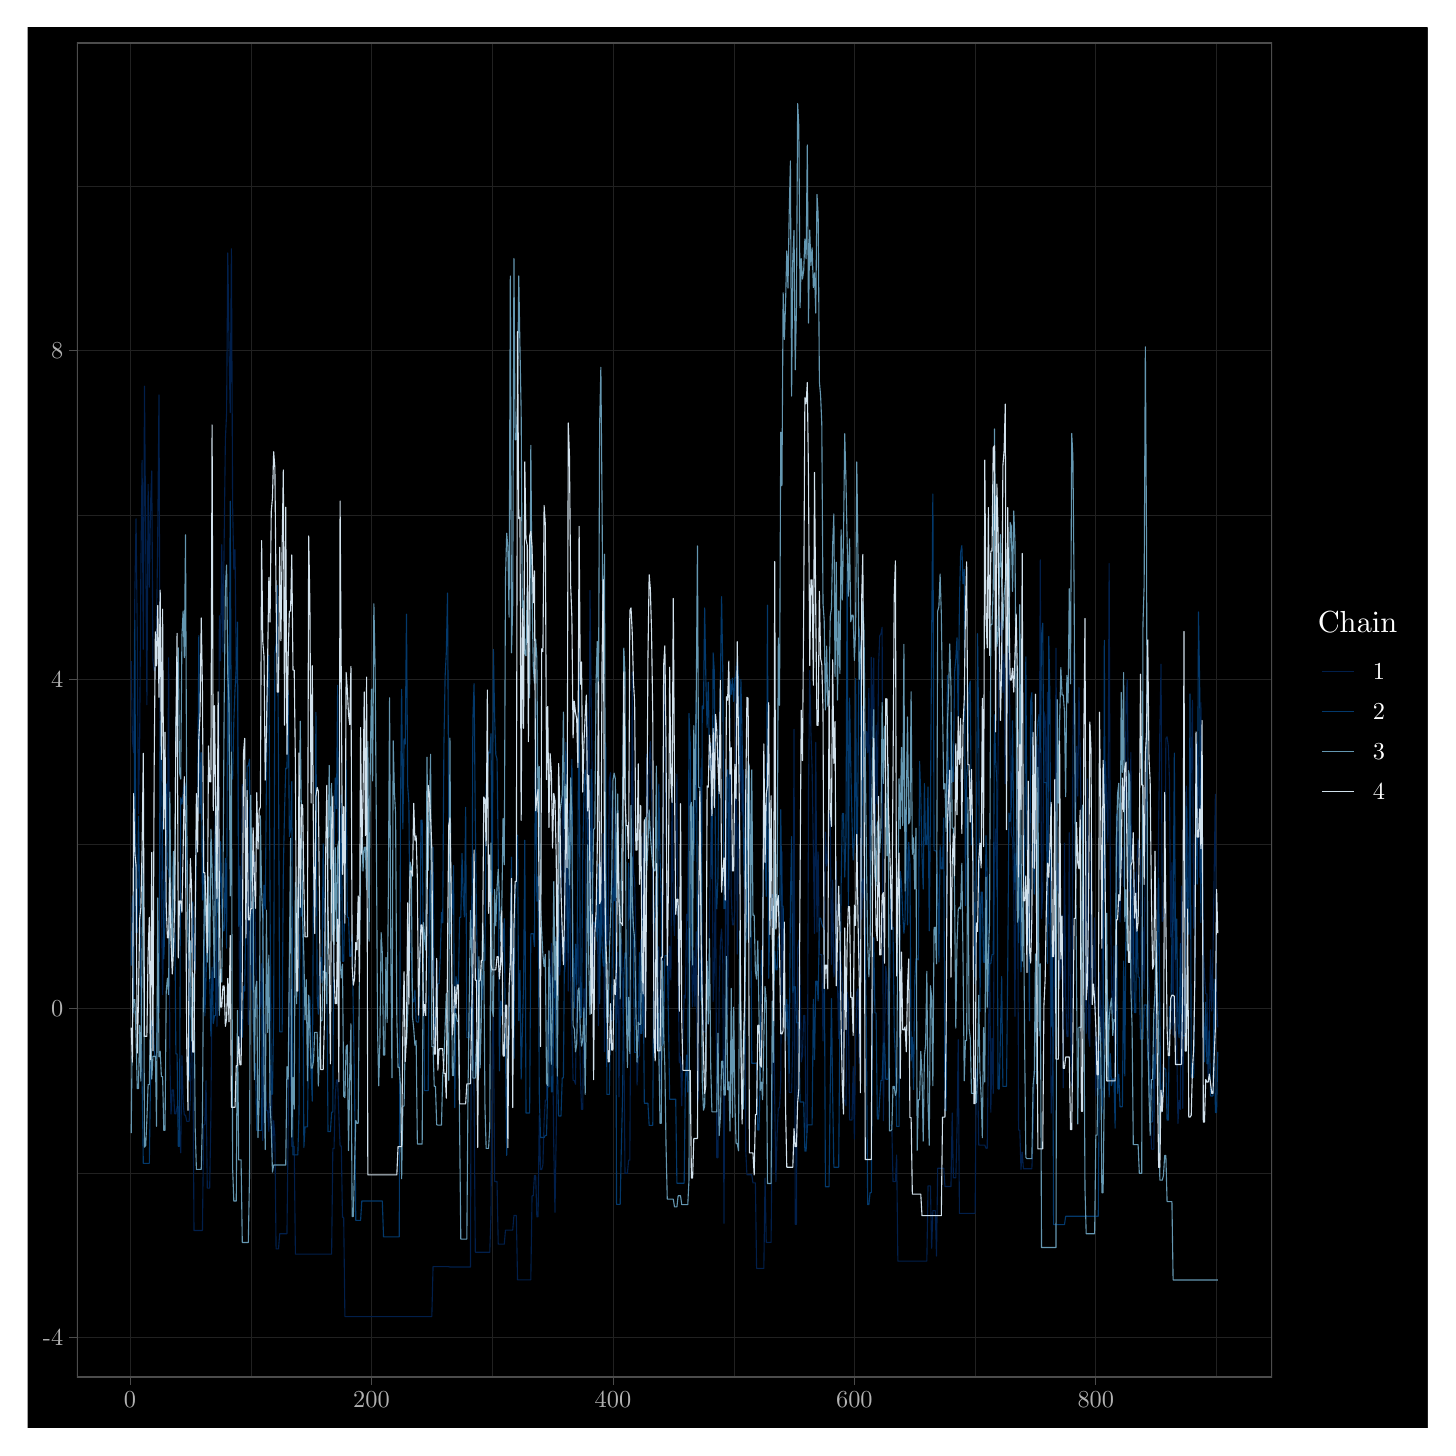
\begin{tikzpicture}[x=1pt,y=1pt]
\definecolor{fillColor}{RGB}{255,255,255}
\path[use as bounding box,fill=fillColor,fill opacity=0.00] (0,0) rectangle (505.89,505.89);
\begin{scope}
\path[clip] (  0.00,  0.00) rectangle (505.89,505.89);
\definecolor{drawColor}{RGB}{0,0,0}
\definecolor{fillColor}{RGB}{0,0,0}

\path[draw=drawColor,line width= 0.6pt,line join=round,line cap=round,fill=fillColor] (  0.00,  0.00) rectangle (505.89,505.89);
\end{scope}
\begin{scope}
\path[clip] ( 17.78, 18.22) rectangle (449.67,500.39);
\definecolor{fillColor}{RGB}{0,0,0}

\path[fill=fillColor] ( 17.78, 18.22) rectangle (449.67,500.39);
\definecolor{drawColor}{gray}{0.13}

\path[draw=drawColor,line width= 0.1pt,line join=round] ( 17.78, 92.03) --
	(449.67, 92.03);

\path[draw=drawColor,line width= 0.1pt,line join=round] ( 17.78,210.94) --
	(449.67,210.94);

\path[draw=drawColor,line width= 0.1pt,line join=round] ( 17.78,329.85) --
	(449.67,329.85);

\path[draw=drawColor,line width= 0.1pt,line join=round] ( 17.78,448.77) --
	(449.67,448.77);

\path[draw=drawColor,line width= 0.1pt,line join=round] ( 80.60, 18.22) --
	( 80.60,500.39);

\path[draw=drawColor,line width= 0.1pt,line join=round] (167.85, 18.22) --
	(167.85,500.39);

\path[draw=drawColor,line width= 0.1pt,line join=round] (255.10, 18.22) --
	(255.10,500.39);

\path[draw=drawColor,line width= 0.1pt,line join=round] (342.36, 18.22) --
	(342.36,500.39);

\path[draw=drawColor,line width= 0.1pt,line join=round] (429.61, 18.22) --
	(429.61,500.39);

\path[draw=drawColor,line width= 0.3pt,line join=round] ( 17.78, 32.57) --
	(449.67, 32.57);

\path[draw=drawColor,line width= 0.3pt,line join=round] ( 17.78,151.48) --
	(449.67,151.48);

\path[draw=drawColor,line width= 0.3pt,line join=round] ( 17.78,270.40) --
	(449.67,270.40);

\path[draw=drawColor,line width= 0.3pt,line join=round] ( 17.78,389.31) --
	(449.67,389.31);

\path[draw=drawColor,line width= 0.3pt,line join=round] ( 36.98, 18.22) --
	( 36.98,500.39);

\path[draw=drawColor,line width= 0.3pt,line join=round] (124.23, 18.22) --
	(124.23,500.39);

\path[draw=drawColor,line width= 0.3pt,line join=round] (211.48, 18.22) --
	(211.48,500.39);

\path[draw=drawColor,line width= 0.3pt,line join=round] (298.73, 18.22) --
	(298.73,500.39);

\path[draw=drawColor,line width= 0.3pt,line join=round] (385.98, 18.22) --
	(385.98,500.39);
\definecolor{drawColor}{RGB}{1,31,75}

\path[draw=drawColor,line width= 0.4pt,line join=round] ( 37.41,276.95) --
	( 37.85,248.28) --
	( 38.29,243.86) --
	( 38.72,300.69) --
	( 39.16,328.42) --
	( 39.59,288.06) --
	( 40.03,221.92) --
	( 40.47,247.74) --
	( 40.90,309.77) --
	( 41.34,349.54) --
	( 41.78,281.23) --
	( 42.21,376.34) --
	( 42.65,320.53) --
	( 43.08,261.24) --
	( 43.52,340.86) --
	( 43.96,303.73) --
	( 44.39,333.10) --
	( 44.83,345.73) --
	( 45.27,277.22) --
	( 45.70,273.55) --
	( 46.14,273.55) --
	( 46.57,288.22) --
	( 47.01,324.22) --
	( 47.45,373.16) --
	( 47.88,242.39) --
	( 48.32,192.88) --
	( 48.76,156.49) --
	( 49.19,182.82) --
	( 49.63,200.56) --
	( 50.06,212.34) --
	( 50.50,213.83) --
	( 50.94,278.22) --
	( 51.37,132.81) --
	( 51.81,113.32) --
	( 52.25,122.08) --
	( 52.68,122.08) --
	( 53.12,113.41) --
	( 53.55,113.41) --
	( 53.99,116.05) --
	( 54.43,116.05) --
	( 54.86,106.66) --
	( 55.30, 99.30) --
	( 55.74,134.45) --
	( 56.17,117.60) --
	( 56.61,112.96) --
	( 57.04,112.96) --
	( 57.48,110.69) --
	( 57.92,110.69) --
	( 58.35,110.69) --
	( 58.79,119.38) --
	( 59.23,141.66) --
	( 59.66,141.66) --
	( 60.10, 71.25) --
	( 60.53, 71.25) --
	( 60.97, 71.25) --
	( 61.41, 71.25) --
	( 61.84, 71.25) --
	( 62.28, 71.25) --
	( 62.72, 71.25) --
	( 63.15, 71.25) --
	( 63.59,109.48) --
	( 64.02,109.48) --
	( 64.46,125.39) --
	( 64.90, 86.55) --
	( 65.33, 86.55) --
	( 65.77, 86.55) --
	( 66.21,112.92) --
	( 66.64,164.63) --
	( 67.08,157.78) --
	( 67.51,207.23) --
	( 67.95,230.79) --
	( 68.39,145.00) --
	( 68.82,161.23) --
	( 69.26,293.37) --
	( 69.70,277.11) --
	( 70.13,319.08) --
	( 70.57,280.24) --
	( 71.00,320.56) --
	( 71.44,357.01) --
	( 71.88,366.65) --
	( 72.31,424.49) --
	( 72.75,390.85) --
	( 73.19,366.80) --
	( 73.62,425.98) --
	( 74.06,333.32) --
	( 74.49,310.15) --
	( 74.93,317.25) --
	( 75.37,269.15) --
	( 75.80,269.15) --
	( 76.24,208.09) --
	( 76.68,134.20) --
	( 77.11,168.96) --
	( 77.55,232.39) --
	( 77.98,231.78) --
	( 78.42,219.06) --
	( 78.86,198.04) --
	( 79.29,213.50) --
	( 79.73,145.61) --
	( 80.17,224.12) --
	( 80.60,209.42) --
	( 81.04,158.13) --
	( 81.47,204.61) --
	( 81.91,206.84) --
	( 82.35,171.96) --
	( 82.78,151.51) --
	( 83.22,151.51) --
	( 83.66,151.51) --
	( 84.09,152.12) --
	( 84.53,167.63) --
	( 84.96,103.76) --
	( 85.40,149.23) --
	( 85.84,131.76) --
	( 86.27,114.60) --
	( 86.71,114.60) --
	( 87.15,107.06) --
	( 87.58,130.80) --
	( 88.02,130.80) --
	( 88.45, 96.96) --
	( 88.89,110.93) --
	( 89.33,105.11) --
	( 89.76, 64.60) --
	( 90.20, 64.60) --
	( 90.64, 64.60) --
	( 91.07, 70.09) --
	( 91.51, 70.09) --
	( 91.95, 70.09) --
	( 92.38, 70.09) --
	( 92.82, 70.09) --
	( 93.25, 70.09) --
	( 93.69, 70.09) --
	( 94.13,107.95) --
	( 94.56,172.53) --
	( 95.00,128.13) --
	( 95.44,101.66) --
	( 95.87,101.66) --
	( 96.31,101.66) --
	( 96.74, 62.72) --
	( 97.18, 62.72) --
	( 97.62, 62.72) --
	( 98.05, 62.72) --
	( 98.49, 62.72) --
	( 98.93, 62.72) --
	( 99.36, 62.72) --
	( 99.80, 62.72) --
	(100.23, 62.72) --
	(100.67, 62.72) --
	(101.11, 62.72) --
	(101.54, 62.72) --
	(101.98, 62.72) --
	(102.42, 62.72) --
	(102.85, 62.72) --
	(103.29, 62.72) --
	(103.72, 62.72) --
	(104.16, 62.72) --
	(104.60, 62.72) --
	(105.03, 62.72) --
	(105.47, 62.72) --
	(105.91, 62.72) --
	(106.34, 62.72) --
	(106.78, 62.72) --
	(107.21, 62.72) --
	(107.65, 62.72) --
	(108.09, 62.72) --
	(108.52, 62.72) --
	(108.96, 62.72) --
	(109.40, 62.72) --
	(109.83, 62.72) --
	(110.27,100.81) --
	(110.70,100.81) --
	(111.14,119.73) --
	(111.58,125.66) --
	(112.01,125.66) --
	(112.45,112.75) --
	(112.89,101.82) --
	(113.32,101.82) --
	(113.76, 75.99) --
	(114.19, 75.99) --
	(114.63, 40.14) --
	(115.07, 40.14) --
	(115.50, 40.14) --
	(115.94, 40.14) --
	(116.38, 40.14) --
	(116.81, 40.14) --
	(117.25, 40.14) --
	(117.68, 40.14) --
	(118.12, 40.14) --
	(118.56, 40.14) --
	(118.99, 40.14) --
	(119.43, 40.14) --
	(119.87, 40.14) --
	(120.30, 40.14) --
	(120.74, 40.14) --
	(121.17, 40.14) --
	(121.61, 40.14) --
	(122.05, 40.14) --
	(122.48, 40.14) --
	(122.92, 40.14) --
	(123.36, 40.14) --
	(123.79, 40.14) --
	(124.23, 40.14) --
	(124.66, 40.14) --
	(125.10, 40.14) --
	(125.54, 40.14) --
	(125.97, 40.14) --
	(126.41, 40.14) --
	(126.85, 40.14) --
	(127.28, 40.14) --
	(127.72, 40.14) --
	(128.15, 40.14) --
	(128.59, 40.14) --
	(129.03, 40.14) --
	(129.46, 40.14) --
	(129.90, 40.14) --
	(130.34, 40.14) --
	(130.77, 40.14) --
	(131.21, 40.14) --
	(131.64, 40.14) --
	(132.08, 40.14) --
	(132.52, 40.14) --
	(132.95, 40.14) --
	(133.39, 40.14) --
	(133.83, 40.14) --
	(134.26, 40.14) --
	(134.70, 40.14) --
	(135.13, 40.14) --
	(135.57, 40.14) --
	(136.01, 40.14) --
	(136.44, 40.14) --
	(136.88, 40.14) --
	(137.32, 40.14) --
	(137.75, 40.14) --
	(138.19, 40.14) --
	(138.62, 40.14) --
	(139.06, 40.14) --
	(139.50, 40.14) --
	(139.93, 40.14) --
	(140.37, 40.14) --
	(140.81, 40.14) --
	(141.24, 40.14) --
	(141.68, 40.14) --
	(142.11, 40.14) --
	(142.55, 40.14) --
	(142.99, 40.14) --
	(143.42, 40.14) --
	(143.86, 40.14) --
	(144.30, 40.14) --
	(144.73, 40.14) --
	(145.17, 40.14) --
	(145.60, 40.14) --
	(146.04, 40.14) --
	(146.48, 58.17) --
	(146.91, 58.17) --
	(147.35, 58.17) --
	(147.79, 58.17) --
	(148.22, 58.17) --
	(148.66, 58.17) --
	(149.09, 58.17) --
	(149.53, 58.17) --
	(149.97, 58.17) --
	(150.40, 58.17) --
	(150.84, 58.17) --
	(151.28, 58.17) --
	(151.71, 58.17) --
	(152.15, 58.17) --
	(152.58, 58.06) --
	(153.02, 58.06) --
	(153.46, 58.06) --
	(153.89, 58.06) --
	(154.33, 58.06) --
	(154.77, 58.06) --
	(155.20, 58.06) --
	(155.64, 58.06) --
	(156.07, 58.06) --
	(156.51, 58.06) --
	(156.95, 58.06) --
	(157.38, 58.06) --
	(157.82, 58.06) --
	(158.26, 58.06) --
	(158.69, 58.06) --
	(159.13, 58.06) --
	(159.56, 58.06) --
	(160.00, 58.06) --
	(160.44,192.08) --
	(160.87,167.83) --
	(161.31,118.53) --
	(161.75, 63.40) --
	(162.18, 63.40) --
	(162.62, 63.40) --
	(163.05, 63.40) --
	(163.49, 63.40) --
	(163.93, 63.40) --
	(164.36, 63.40) --
	(164.80, 63.40) --
	(165.24, 63.40) --
	(165.67, 63.40) --
	(166.11, 63.40) --
	(166.54, 63.40) --
	(166.98, 63.40) --
	(167.42, 77.22) --
	(167.85,137.75) --
	(168.29,149.18) --
	(168.73, 88.96) --
	(169.16, 88.96) --
	(169.60, 88.96) --
	(170.03, 66.31) --
	(170.47, 66.31) --
	(170.91, 66.31) --
	(171.34, 66.31) --
	(171.78, 66.31) --
	(172.22, 66.31) --
	(172.65, 71.39) --
	(173.09, 71.39) --
	(173.52, 71.39) --
	(173.96, 71.39) --
	(174.40, 71.39) --
	(174.83, 71.39) --
	(175.27, 71.39) --
	(175.71, 76.65) --
	(176.14, 76.65) --
	(176.58, 76.65) --
	(177.01, 53.42) --
	(177.45, 53.42) --
	(177.89, 53.42) --
	(178.32, 53.42) --
	(178.76, 53.42) --
	(179.20, 53.42) --
	(179.63, 53.42) --
	(180.07, 53.42) --
	(180.50, 53.42) --
	(180.94, 53.42) --
	(181.38, 53.42) --
	(181.81, 53.42) --
	(182.25, 83.79) --
	(182.69, 83.79) --
	(183.12, 91.11) --
	(183.56, 91.11) --
	(183.99, 76.18) --
	(184.43, 76.18) --
	(184.87,112.79) --
	(185.30, 93.26) --
	(185.74, 93.26) --
	(186.18, 95.05) --
	(186.61,110.67) --
	(187.05,118.36) --
	(187.49,118.36) --
	(187.92,147.23) --
	(188.36,140.55) --
	(188.79,142.32) --
	(189.23,174.90) --
	(189.67,139.21) --
	(190.10,102.18) --
	(190.54, 77.83) --
	(190.98,105.69) --
	(191.41,141.21) --
	(191.85,196.78) --
	(192.28,163.53) --
	(192.72,173.68) --
	(193.16,218.97) --
	(193.59,235.60) --
	(194.03,164.55) --
	(194.47,168.89) --
	(194.90,220.72) --
	(195.34,157.79) --
	(195.77,225.45) --
	(196.21,163.34) --
	(196.65,144.50) --
	(197.08,125.50) --
	(197.52,125.50) --
	(197.96,124.11) --
	(198.39,163.04) --
	(198.83,180.93) --
	(199.26,153.44) --
	(199.70,128.85) --
	(200.14,115.02) --
	(200.57,115.02) --
	(201.01,158.59) --
	(201.45,142.24) --
	(201.88,262.11) --
	(202.32,254.60) --
	(202.75,206.52) --
	(203.19,302.57) --
	(203.63,263.39) --
	(204.06,226.85) --
	(204.50,153.78) --
	(204.94,182.31) --
	(205.37,180.35) --
	(205.81,194.50) --
	(206.24,145.27) --
	(206.68,180.40) --
	(207.12,206.22) --
	(207.55,177.47) --
	(207.99,214.65) --
	(208.43,135.90) --
	(208.86,206.00) --
	(209.30,183.54) --
	(209.73,174.39) --
	(210.17,233.92) --
	(210.61,236.68) --
	(211.04,214.16) --
	(211.48,189.10) --
	(211.92,196.64) --
	(212.35,232.92) --
	(212.79,146.33) --
	(213.22,171.81) --
	(213.66,119.52) --
	(214.10,159.57) --
	(214.53,176.57) --
	(214.97,154.32) --
	(215.41,141.76) --
	(215.84, 91.93) --
	(216.28, 91.93) --
	(216.71, 91.93) --
	(217.15, 96.68) --
	(217.59, 96.68) --
	(218.02,175.09) --
	(218.46,272.95) --
	(218.90,200.79) --
	(219.33,197.96) --
	(219.77,176.58) --
	(220.20,123.81) --
	(220.64,134.27) --
	(221.08,134.27) --
	(221.51,176.55) --
	(221.95,151.62) --
	(222.39,214.84) --
	(222.82,145.25) --
	(223.26,143.45) --
	(223.69,243.39) --
	(224.13,220.74) --
	(224.57,239.71) --
	(225.00,247.93) --
	(225.44,232.95) --
	(225.88,198.99) --
	(226.31,148.94) --
	(226.75,148.94) --
	(227.18,137.06) --
	(227.62,173.68) --
	(228.06,173.68) --
	(228.49,119.36) --
	(228.93,157.69) --
	(229.37,167.15) --
	(229.80,254.50) --
	(230.24,277.23) --
	(230.67,214.52) --
	(231.11,184.92) --
	(231.55,154.35) --
	(231.98,174.03) --
	(232.42,161.80) --
	(232.86,237.49) --
	(233.29,187.31) --
	(233.73,177.85) --
	(234.16,205.55) --
	(234.60,236.14) --
	(235.04,165.94) --
	(235.47,131.82) --
	(235.91,134.07) --
	(236.35,116.27) --
	(236.78,140.53) --
	(237.22,156.24) --
	(237.65,155.22) --
	(238.09,185.55) --
	(238.53,183.24) --
	(238.96,236.57) --
	(239.40,225.78) --
	(239.84,173.26) --
	(240.27,152.09) --
	(240.71,172.44) --
	(241.14,152.23) --
	(241.58,179.23) --
	(242.02,116.83) --
	(242.45,120.13) --
	(242.89,219.87) --
	(243.33,238.49) --
	(243.76,166.33) --
	(244.20,143.03) --
	(244.63,143.03) --
	(245.07,143.03) --
	(245.51,146.85) --
	(245.94,146.85) --
	(246.38,185.52) --
	(246.82,209.65) --
	(247.25,243.06) --
	(247.69,154.05) --
	(248.12,165.48) --
	(248.56,209.57) --
	(249.00, 97.55) --
	(249.43, 97.55) --
	(249.87,157.23) --
	(250.31,175.81) --
	(250.74,180.20) --
	(251.18,168.18) --
	(251.61, 73.86) --
	(252.05,168.17) --
	(252.49,237.70) --
	(252.92,147.50) --
	(253.36,203.47) --
	(253.80,247.17) --
	(254.23,192.46) --
	(254.67,181.69) --
	(255.10,181.70) --
	(255.54,186.85) --
	(255.98,275.16) --
	(256.41,171.14) --
	(256.85,217.00) --
	(257.29,220.84) --
	(257.72,251.90) --
	(258.16,221.32) --
	(258.59,237.65) --
	(259.03,191.99) --
	(259.47,100.10) --
	(259.90, 91.38) --
	(260.34, 91.38) --
	(260.78, 91.38) --
	(261.21, 91.38) --
	(261.65, 91.38) --
	(262.08, 88.44) --
	(262.52, 88.44) --
	(262.96, 88.44) --
	(263.39, 57.55) --
	(263.83, 57.55) --
	(264.27, 57.55) --
	(264.70, 57.55) --
	(265.14, 57.55) --
	(265.57, 57.55) --
	(266.01, 57.55) --
	(266.45, 90.19) --
	(266.88, 66.94) --
	(267.32, 66.94) --
	(267.76, 66.94) --
	(268.19, 66.94) --
	(268.63, 66.94) --
	(269.06,114.66) --
	(269.50,156.48) --
	(269.94,119.15) --
	(270.37, 88.86) --
	(270.81,106.05) --
	(271.25,115.56) --
	(271.68,115.56) --
	(272.12,125.07) --
	(272.55,208.28) --
	(272.99,152.73) --
	(273.43,152.73) --
	(273.86,152.73) --
	(274.30,152.73) --
	(274.74,152.73) --
	(275.17,121.17) --
	(275.61,121.17) --
	(276.04,121.17) --
	(276.48,139.70) --
	(276.92,252.34) --
	(277.35, 73.46) --
	(277.79, 73.46) --
	(278.23,173.16) --
	(278.66,176.21) --
	(279.10,162.41) --
	(279.53,132.17) --
	(279.97,134.59) --
	(280.41,148.94) --
	(280.84,148.94) --
	(281.28,106.62) --
	(281.72,106.62) --
	(282.15,228.80) --
	(282.59,273.66) --
	(283.02,251.45) --
	(283.46,237.72) --
	(283.90,208.85) --
	(284.33,178.59) --
	(284.77,247.58) --
	(285.21,179.10) --
	(285.64,208.00) --
	(286.08,170.92) --
	(286.52,170.92) --
	(286.95,170.92) --
	(287.39,139.74) --
	(287.82,165.43) --
	(288.26,215.21) --
	(288.70,202.96) --
	(289.13,205.59) --
	(289.57,220.76) --
	(290.01,222.62) --
	(290.44,167.44) --
	(290.88,197.87) --
	(291.31,162.86) --
	(291.75,166.36) --
	(292.19,204.57) --
	(292.62,160.49) --
	(293.06,140.56) --
	(293.50,175.34) --
	(293.93,168.06) --
	(294.37,160.00) --
	(294.80,118.32) --
	(295.24,118.32) --
	(295.68,116.33) --
	(296.11,157.27) --
	(296.55,153.45) --
	(296.99,111.18) --
	(297.42,111.18) --
	(297.86,111.18) --
	(298.29,130.60) --
	(298.73,104.33) --
	(299.17,138.99) --
	(299.60,157.46) --
	(300.04,158.61) --
	(300.48,131.68) --
	(300.91,216.84) --
	(301.35,183.71) --
	(301.78,198.35) --
	(302.22,191.44) --
	(302.66,242.18) --
	(303.09,251.61) --
	(303.53,243.88) --
	(303.97,267.14) --
	(304.40,187.45) --
	(304.84,278.36) --
	(305.27,249.00) --
	(305.71,278.10) --
	(306.15,205.68) --
	(306.58,253.77) --
	(307.02,225.35) --
	(307.46,275.28) --
	(307.89,286.15) --
	(308.33,286.88) --
	(308.76,289.22) --
	(309.20,110.91) --
	(309.64,142.27) --
	(310.07,166.66) --
	(310.51,161.59) --
	(310.95,142.92) --
	(311.38,109.30) --
	(311.82,109.30) --
	(312.25,109.30) --
	(312.69, 88.89) --
	(313.13, 88.89) --
	(313.56, 88.89) --
	(314.00, 98.51) --
	(314.44, 60.19) --
	(314.87, 60.19) --
	(315.31, 60.19) --
	(315.74, 60.19) --
	(316.18, 60.19) --
	(316.62, 60.19) --
	(317.05, 60.19) --
	(317.49, 60.19) --
	(317.93, 60.19) --
	(318.36, 60.19) --
	(318.80, 60.19) --
	(319.23, 60.19) --
	(319.67, 60.19) --
	(320.11, 60.19) --
	(320.54, 60.19) --
	(320.98, 60.19) --
	(321.42, 60.19) --
	(321.85, 60.19) --
	(322.29, 60.19) --
	(322.72, 60.19) --
	(323.16, 60.19) --
	(323.60, 60.19) --
	(324.03, 60.19) --
	(324.47, 60.19) --
	(324.91, 60.19) --
	(325.34, 87.36) --
	(325.78, 87.36) --
	(326.21, 87.36) --
	(326.65, 64.82) --
	(327.09, 78.41) --
	(327.52, 78.41) --
	(327.96, 78.41) --
	(328.40, 61.97) --
	(328.83, 93.74) --
	(329.27, 93.74) --
	(329.70, 93.74) --
	(330.14, 93.74) --
	(330.58, 93.74) --
	(331.01, 93.74) --
	(331.45, 87.14) --
	(331.89, 87.14) --
	(332.32, 87.14) --
	(332.76, 87.14) --
	(333.19, 87.14) --
	(333.63, 87.14) --
	(334.07,113.75) --
	(334.50, 90.29) --
	(334.94, 90.29) --
	(335.38, 90.29) --
	(335.81,107.24) --
	(336.25,140.21) --
	(336.68, 77.41) --
	(337.12, 77.41) --
	(337.56, 77.41) --
	(337.99, 77.41) --
	(338.43, 77.41) --
	(338.87, 77.41) --
	(339.30, 77.41) --
	(339.74, 77.41) --
	(340.17, 77.41) --
	(340.61, 77.41) --
	(341.05, 77.41) --
	(341.48, 77.41) --
	(341.92, 77.41) --
	(342.36, 77.41) --
	(342.79,129.59) --
	(343.23,129.59) --
	(343.66,102.11) --
	(344.10,102.11) --
	(344.54,102.11) --
	(344.97,102.11) --
	(345.41,102.11) --
	(345.85,102.11) --
	(346.28,100.97) --
	(346.72,100.97) --
	(347.15,136.83) --
	(347.59,174.15) --
	(348.03,113.97) --
	(348.46,140.63) --
	(348.90,120.77) --
	(349.34,206.89) --
	(349.77,216.35) --
	(350.21,194.45) --
	(350.64,240.11) --
	(351.08,291.97) --
	(351.52,286.31) --
	(351.95,295.62) --
	(352.39,265.70) --
	(352.83,279.55) --
	(353.26,232.68) --
	(353.70,249.75) --
	(354.13,263.26) --
	(354.57,300.61) --
	(355.01,238.37) --
	(355.44,214.30) --
	(355.88,213.00) --
	(356.32,194.04) --
	(356.75,148.63) --
	(357.19,216.11) --
	(357.62,241.55) --
	(358.06,107.51) --
	(358.50,107.51) --
	(358.93, 93.38) --
	(359.37, 99.53) --
	(359.81, 93.56) --
	(360.24, 93.56) --
	(360.68, 93.56) --
	(361.11, 93.56) --
	(361.55, 93.56) --
	(361.99, 93.56) --
	(362.42, 93.56) --
	(362.86, 93.56) --
	(363.30,105.35) --
	(363.73,128.61) --
	(364.17,128.61) --
	(364.60,128.61) --
	(365.04,246.66) --
	(365.48,218.62) --
	(365.91,313.60) --
	(366.35,184.08) --
	(366.79,193.70) --
	(367.22,258.71) --
	(367.66,256.56) --
	(368.09,227.86) --
	(368.53,265.74) --
	(368.97,182.22) --
	(369.40,182.14) --
	(369.84,113.63) --
	(370.28,125.53) --
	(370.71,139.69) --
	(371.15,178.90) --
	(371.58,281.65) --
	(372.02,194.05) --
	(372.46,203.94) --
	(372.89,161.67) --
	(373.33,166.76) --
	(373.77,185.31) --
	(374.20,122.84) --
	(374.64,211.23) --
	(375.07,155.92) --
	(375.51,141.34) --
	(375.95,141.34) --
	(376.38,214.99) --
	(376.82,146.79) --
	(377.26,123.62) --
	(377.69,245.76) --
	(378.13,282.43) --
	(378.56,199.33) --
	(379.00,246.14) --
	(379.44,228.21) --
	(379.87,267.46) --
	(380.31,243.27) --
	(380.75,213.46) --
	(381.18,211.92) --
	(381.62,202.89) --
	(382.06,172.84) --
	(382.49,142.45) --
	(382.93,234.43) --
	(383.36,141.13) --
	(383.80,137.78) --
	(384.24,214.96) --
	(384.67,152.96) --
	(385.11,169.19) --
	(385.55,184.21) --
	(385.98,119.85) --
	(386.42,141.15) --
	(386.85,122.26) --
	(387.29,164.45) --
	(387.73,147.66) --
	(388.16,139.27) --
	(388.60,234.75) --
	(389.04,211.99) --
	(389.47,240.63) --
	(389.91,226.36) --
	(390.34,211.54) --
	(390.78,312.21) --
	(391.22,194.93) --
	(391.65,160.42) --
	(392.09,144.49) --
	(392.53,174.11) --
	(392.96,124.06) --
	(393.40,184.65) --
	(393.83,223.08) --
	(394.27,198.01) --
	(394.71,182.70) --
	(395.14,209.54) --
	(395.58,209.54) --
	(396.02,195.55) --
	(396.45,207.14) --
	(396.89,262.46) --
	(397.32,270.41) --
	(397.76,222.00) --
	(398.20,193.89) --
	(398.63,243.98) --
	(399.07,150.62) --
	(399.51,194.47) --
	(399.94,200.66) --
	(400.38,164.61) --
	(400.81,203.71) --
	(401.25,212.82) --
	(401.69,205.65) --
	(402.12,208.87) --
	(402.56,155.85) --
	(403.00,180.83) --
	(403.43,158.67) --
	(403.87,219.47) --
	(404.30,265.01) --
	(404.74,163.46) --
	(405.18,158.70) --
	(405.61,124.34) --
	(406.05,100.66) --
	(406.49,100.66) --
	(406.92,100.66) --
	(407.36,141.52) --
	(407.79,170.04) --
	(408.23,170.04) --
	(408.67,218.53) --
	(409.10,251.65) --
	(409.54,275.86) --
	(409.98,182.93) --
	(410.41,184.30) --
	(410.85,184.30) --
	(411.28,249.01) --
	(411.72,249.66) --
	(412.16,246.48) --
	(412.59,233.74) --
	(413.03,177.32) --
	(413.47,204.17) --
	(413.90,141.83) --
	(414.34,197.27) --
	(414.77,180.53) --
	(415.21,137.81) --
	(415.65,109.94) --
	(416.08,118.26) --
	(416.52,115.02) --
	(416.96,195.70) --
	(417.39,115.40) --
	(417.83,162.10) --
	(418.26,146.73) --
	(418.70,231.81) --
	(419.14,213.98) --
	(419.57,191.61) --
	(420.01,207.24) --
	(420.45,237.77) --
	(420.88,262.84) --
	(421.32,180.52) --
	(421.75,190.02) --
	(422.19,231.51) --
	(422.63,247.77) --
	(423.06,239.56) --
	(423.50,198.85) --
	(423.94,261.98) --
	(424.37,214.73) --
	(424.81,173.60) --
	(425.24,163.43) --
	(425.68,156.75) --
	(426.12,156.75) --
	(426.55,126.27) --
	(426.99,144.02) --
	(427.43,172.63) --
	(427.86,150.57) --
	(428.30,170.49) --
	(428.73,200.11) --
	(429.17,228.90) --
	(429.61,154.74) --
	(430.04,144.68);
\definecolor{drawColor}{RGB}{3,57,108}

\path[draw=drawColor,line width= 0.4pt,line join=round] ( 37.41,166.99) --
	( 37.85,192.15) --
	( 38.29,149.86) --
	( 38.72,291.74) --
	( 39.16,178.87) --
	( 39.59,178.87) --
	( 40.03,220.96) --
	( 40.47,192.37) --
	( 40.90,157.60) --
	( 41.34,126.27) --
	( 41.78, 95.52) --
	( 42.21, 95.52) --
	( 42.65, 95.52) --
	( 43.08, 95.52) --
	( 43.52, 95.52) --
	( 43.96, 95.52) --
	( 44.39,126.38) --
	( 44.83,146.59) --
	( 45.27,148.43) --
	( 45.70,136.26) --
	( 46.14,133.41) --
	( 46.57,133.41) --
	( 47.01,164.59) --
	( 47.45,149.95) --
	( 47.88,255.46) --
	( 48.32,248.69) --
	( 48.76,203.63) --
	( 49.19,169.38) --
	( 49.63,182.82) --
	( 50.06,232.65) --
	( 50.50,201.84) --
	( 50.94,201.84) --
	( 51.37,195.18) --
	( 51.81,182.99) --
	( 52.25,184.29) --
	( 52.68,207.66) --
	( 53.12,190.53) --
	( 53.55,135.06) --
	( 53.99,135.06) --
	( 54.43,101.63) --
	( 54.86,101.63) --
	( 55.30,227.63) --
	( 55.74,225.34) --
	( 56.17,228.86) --
	( 56.61,233.50) --
	( 57.04,231.16) --
	( 57.48,203.81) --
	( 57.92,181.99) --
	( 58.35,125.19) --
	( 58.79,175.24) --
	( 59.23,171.71) --
	( 59.66,189.99) --
	( 60.10,165.36) --
	( 60.53,165.36) --
	( 60.97,217.70) --
	( 61.41,217.70) --
	( 61.84,286.20) --
	( 62.28,221.96) --
	( 62.72,243.92) --
	( 63.15,190.63) --
	( 63.59,219.96) --
	( 64.02,148.78) --
	( 64.46,162.57) --
	( 64.90,182.48) --
	( 65.33,182.48) --
	( 65.77,163.11) --
	( 66.21,141.49) --
	( 66.64,166.36) --
	( 67.08,146.03) --
	( 67.51,148.90) --
	( 67.95,148.90) --
	( 68.39,219.62) --
	( 68.82,186.27) --
	( 69.26,186.27) --
	( 69.70,211.74) --
	( 70.13,187.90) --
	( 70.57,179.57) --
	( 71.00,179.57) --
	( 71.44,205.77) --
	( 71.88,173.29) --
	( 72.31,286.56) --
	( 72.75,239.64) --
	( 73.19,334.79) --
	( 73.62,237.19) --
	( 74.06,234.36) --
	( 74.49,255.23) --
	( 74.93,266.72) --
	( 75.37,274.33) --
	( 75.80,291.10) --
	( 76.24,181.15) --
	( 76.68,202.96) --
	( 77.11,141.08) --
	( 77.55,141.08) --
	( 77.98,159.40) --
	( 78.42,157.73) --
	( 78.86,184.99) --
	( 79.29,239.11) --
	( 79.73,239.11) --
	( 80.17,241.54) --
	( 80.60,184.36) --
	( 81.04,186.68) --
	( 81.47,148.17) --
	( 81.91,131.58) --
	( 82.35,131.58) --
	( 82.78,107.41) --
	( 83.22,107.41) --
	( 83.66,107.41) --
	( 84.09,107.41) --
	( 84.53,107.41) --
	( 84.96,177.82) --
	( 85.40,196.02) --
	( 85.84,187.31) --
	( 86.27,233.75) --
	( 86.71,273.67) --
	( 87.15,279.16) --
	( 87.58,190.43) --
	( 88.02,120.49) --
	( 88.45,120.49) --
	( 88.89,149.17) --
	( 89.33,279.70) --
	( 89.76,283.07) --
	( 90.20,304.31) --
	( 90.64,239.85) --
	( 91.07,143.03) --
	( 91.51,143.03) --
	( 91.95,143.03) --
	( 92.38,201.28) --
	( 92.82,222.73) --
	( 93.25,238.28) --
	( 93.69,238.28) --
	( 94.13,266.53) --
	( 94.56,213.60) --
	( 95.00,216.39) --
	( 95.44,233.47) --
	( 95.87, 98.55) --
	( 96.31, 98.55) --
	( 96.74, 98.55) --
	( 97.18, 98.55) --
	( 97.62, 98.55) --
	( 98.05,113.87) --
	( 98.49,214.14) --
	( 98.93,184.83) --
	( 99.36,188.37) --
	( 99.80,101.23) --
	(100.23,108.71) --
	(100.67,108.71) --
	(101.11,108.71) --
	(101.54,144.65) --
	(101.98,155.68) --
	(102.42,127.59) --
	(102.85,117.98) --
	(103.29,203.86) --
	(103.72,184.57) --
	(104.16,258.49) --
	(104.60,155.80) --
	(105.03,149.40) --
	(105.47,167.20) --
	(105.91,170.01) --
	(106.34,160.81) --
	(106.78,210.99) --
	(107.21,183.79) --
	(107.65,162.58) --
	(108.09,164.01) --
	(108.52,106.95) --
	(108.96,106.95) --
	(109.40,106.95) --
	(109.83,114.03) --
	(110.27,114.03) --
	(110.70,207.16) --
	(111.14,234.75) --
	(111.58,223.66) --
	(112.01,268.28) --
	(112.45,168.17) --
	(112.89,189.36) --
	(113.32,228.62) --
	(113.76,168.49) --
	(114.19,168.49) --
	(114.63,194.52) --
	(115.07,241.28) --
	(115.50,184.41) --
	(115.94,184.41) --
	(116.38,170.36) --
	(116.81,170.36) --
	(117.25,178.23) --
	(117.68,148.58) --
	(118.12,124.02) --
	(118.56, 74.89) --
	(118.99, 74.89) --
	(119.43, 74.89) --
	(119.87, 74.89) --
	(120.30, 74.89) --
	(120.74, 81.91) --
	(121.17, 81.91) --
	(121.61, 81.91) --
	(122.05, 81.91) --
	(122.48, 81.91) --
	(122.92, 81.91) --
	(123.36, 81.91) --
	(123.79, 81.91) --
	(124.23, 81.91) --
	(124.66, 81.91) --
	(125.10, 81.91) --
	(125.54, 81.91) --
	(125.97, 81.91) --
	(126.41, 81.91) --
	(126.85, 81.91) --
	(127.28, 81.91) --
	(127.72, 81.91) --
	(128.15, 81.91) --
	(128.59, 68.96) --
	(129.03, 68.96) --
	(129.46, 68.96) --
	(129.90, 68.96) --
	(130.34, 68.96) --
	(130.77, 68.96) --
	(131.21, 68.96) --
	(131.64, 68.96) --
	(132.08, 68.96) --
	(132.52, 68.96) --
	(132.95, 68.96) --
	(133.39, 68.96) --
	(133.83, 68.96) --
	(134.26, 68.96) --
	(134.70,221.46) --
	(135.13,266.77) --
	(135.57,216.33) --
	(136.01,248.89) --
	(136.44,247.04) --
	(136.88,293.99) --
	(137.32,231.96) --
	(137.75,225.71) --
	(138.19,171.84) --
	(138.62,171.84) --
	(139.06,153.91) --
	(139.50,153.91) --
	(139.93,158.15) --
	(140.37,147.00) --
	(140.81,146.52) --
	(141.24,146.52) --
	(141.68,156.54) --
	(142.11,219.54) --
	(142.55,219.54) --
	(142.99,167.01) --
	(143.42,121.80) --
	(143.86,121.80) --
	(144.30,121.80) --
	(144.73,121.80) --
	(145.17,191.55) --
	(145.60,201.31) --
	(146.04,160.44) --
	(146.48,209.74) --
	(146.91,137.58) --
	(147.35,148.19) --
	(147.79,148.19) --
	(148.22,160.45) --
	(148.66,160.45) --
	(149.09,170.11) --
	(149.53,186.16) --
	(149.97,182.38) --
	(150.40,246.42) --
	(150.84,271.32) --
	(151.28,280.25) --
	(151.71,301.59) --
	(152.15,221.90) --
	(152.58,178.52) --
	(153.02,178.52) --
	(153.46,189.08) --
	(153.89,203.10) --
	(154.33,115.68) --
	(154.77,162.99) --
	(155.20,160.25) --
	(155.64,160.25) --
	(156.07,184.42) --
	(156.51,184.42) --
	(156.95,207.53) --
	(157.38,191.99) --
	(157.82,184.55) --
	(158.26,224.14) --
	(158.69,140.96) --
	(159.13,140.96) --
	(159.56,140.96) --
	(160.00,151.92) --
	(160.44,151.92) --
	(160.87,255.83) --
	(161.31,268.83) --
	(161.75,219.07) --
	(162.18,183.97) --
	(162.62,160.09) --
	(163.05,127.39) --
	(163.49,164.94) --
	(163.93,164.44) --
	(164.36,154.58) --
	(164.80,168.86) --
	(165.24,168.86) --
	(165.67,232.48) --
	(166.11,234.63) --
	(166.54,244.03) --
	(166.98,243.81) --
	(167.42,250.75) --
	(167.85,192.58) --
	(168.29,281.22) --
	(168.73,257.04) --
	(169.16,243.13) --
	(169.60,241.67) --
	(170.03,208.19) --
	(170.47,128.91) --
	(170.91,154.15) --
	(171.34,148.78) --
	(171.78,174.77) --
	(172.22,183.94) --
	(172.65,138.98) --
	(173.09, 98.36) --
	(173.52,138.35) --
	(173.96,138.35) --
	(174.40,181.33) --
	(174.83,206.14) --
	(175.27,142.21) --
	(175.71,133.27) --
	(176.14,189.16) --
	(176.58,198.81) --
	(177.01,214.10) --
	(177.45,147.13) --
	(177.89,165.26) --
	(178.32,125.98) --
	(178.76,143.89) --
	(179.20,160.25) --
	(179.63,212.27) --
	(180.07,113.70) --
	(180.50,113.70) --
	(180.94,113.70) --
	(181.38,113.70) --
	(181.81,178.46) --
	(182.25,178.46) --
	(182.69,178.46) --
	(183.12,173.82) --
	(183.56,263.37) --
	(183.99,190.27) --
	(184.43,199.05) --
	(184.87,120.53) --
	(185.30,104.85) --
	(185.74,104.85) --
	(186.18,104.85) --
	(186.61,104.85) --
	(187.05,105.60) --
	(187.49,105.60) --
	(187.92,123.27) --
	(188.36,123.27) --
	(188.79,164.02) --
	(189.23,121.35) --
	(189.67,121.35) --
	(190.10,151.32) --
	(190.54,177.35) --
	(190.98,130.02) --
	(191.41,130.02) --
	(191.85,112.62) --
	(192.28,112.62) --
	(192.72,112.62) --
	(193.16,126.39) --
	(193.59,126.39) --
	(194.03,180.00) --
	(194.47,247.58) --
	(194.90,193.89) --
	(195.34,171.56) --
	(195.77,196.47) --
	(196.21,211.22) --
	(196.65,241.54) --
	(197.08,174.80) --
	(197.52,151.71) --
	(197.96,174.68) --
	(198.39,160.14) --
	(198.83,206.00) --
	(199.26,281.72) --
	(199.70,148.26) --
	(200.14,148.26) --
	(200.57,207.50) --
	(201.01,228.51) --
	(201.45,237.70) --
	(201.88,233.82) --
	(202.32,214.24) --
	(202.75,204.96) --
	(203.19,174.14) --
	(203.63,237.90) --
	(204.06,182.40) --
	(204.50,182.40) --
	(204.94,181.71) --
	(205.37,184.96) --
	(205.81,175.73) --
	(206.24,203.65) --
	(206.68,153.24) --
	(207.12,193.65) --
	(207.55,173.76) --
	(207.99,166.83) --
	(208.43,166.83) --
	(208.86,247.46) --
	(209.30,120.42) --
	(209.73,120.42) --
	(210.17,120.42) --
	(210.61,147.26) --
	(211.04,147.03) --
	(211.48,195.10) --
	(211.92,190.35) --
	(212.35,213.84) --
	(212.79, 80.67) --
	(213.22, 80.67) --
	(213.66, 80.67) --
	(214.10, 80.67) --
	(214.53,101.80) --
	(214.97,119.94) --
	(215.41,162.79) --
	(215.84,171.58) --
	(216.28,171.58) --
	(216.71,144.46) --
	(217.15,204.01) --
	(217.59,183.78) --
	(218.02,183.78) --
	(218.46,206.28) --
	(218.90,167.88) --
	(219.33,135.61) --
	(219.77,135.61) --
	(220.20,135.61) --
	(220.64,141.02) --
	(221.08,171.68) --
	(221.51,142.47) --
	(221.95,142.47) --
	(222.39,167.31) --
	(222.82,117.22) --
	(223.26,117.22) --
	(223.69,117.22) --
	(224.13,117.22) --
	(224.57,109.23) --
	(225.00,109.23) --
	(225.44,109.23) --
	(225.88,109.23) --
	(226.31,180.95) --
	(226.75,188.68) --
	(227.18,199.89) --
	(227.62,185.10) --
	(228.06,232.52) --
	(228.49,205.91) --
	(228.93,193.33) --
	(229.37,138.06) --
	(229.80,139.51) --
	(230.24,170.52) --
	(230.67,170.52) --
	(231.11,170.52) --
	(231.55,147.25) --
	(231.98,118.68) --
	(232.42,118.68) --
	(232.86,118.68) --
	(233.29,118.68) --
	(233.73,118.68) --
	(234.16,118.68) --
	(234.60, 88.32) --
	(235.04, 88.32) --
	(235.47, 88.32) --
	(235.91, 88.32) --
	(236.35, 88.32) --
	(236.78, 88.32) --
	(237.22, 88.32) --
	(237.65,124.37) --
	(238.09,134.65) --
	(238.53,121.26) --
	(238.96,258.12) --
	(239.40,247.89) --
	(239.84,174.07) --
	(240.27,224.38) --
	(240.71,204.90) --
	(241.14,225.27) --
	(241.58,263.00) --
	(242.02,176.06) --
	(242.45,169.94) --
	(242.89,168.65) --
	(243.33,154.17) --
	(243.76,260.80) --
	(244.20,259.73) --
	(244.63,296.22) --
	(245.07,270.01) --
	(245.51,253.01) --
	(245.94,269.36) --
	(246.38,238.59) --
	(246.82,247.31) --
	(247.25,198.34) --
	(247.69,279.99) --
	(248.12,273.25) --
	(248.56,199.62) --
	(249.00,187.44) --
	(249.43,198.27) --
	(249.87,250.30) --
	(250.31,268.91) --
	(250.74,300.29) --
	(251.18,273.40) --
	(251.61,187.53) --
	(252.05,187.53) --
	(252.49,236.42) --
	(252.92,237.68) --
	(253.36,194.54) --
	(253.80,270.36) --
	(254.23,264.98) --
	(254.67,270.79) --
	(255.10,262.41) --
	(255.54,271.01) --
	(255.98,271.01) --
	(256.41,277.84) --
	(256.85,270.48) --
	(257.29,235.42) --
	(257.72,270.38) --
	(258.16,248.85) --
	(258.59,215.25) --
	(259.03,195.42) --
	(259.47,235.90) --
	(259.90,176.23) --
	(260.34,205.09) --
	(260.78,235.81) --
	(261.21,202.04) --
	(261.65,131.69) --
	(262.08,131.69) --
	(262.52,131.69) --
	(262.96,131.69) --
	(263.39,131.69) --
	(263.83,107.55) --
	(264.27,107.55) --
	(264.70,126.61) --
	(265.14,172.46) --
	(265.57,169.82) --
	(266.01,236.23) --
	(266.45,206.79) --
	(266.88,191.97) --
	(267.32,297.23) --
	(267.76,162.36) --
	(268.19,184.05) --
	(268.63,184.05) --
	(269.06,192.70) --
	(269.50,152.83) --
	(269.94,172.12) --
	(270.37,165.41) --
	(270.81,165.41) --
	(271.25,177.62) --
	(271.68,173.54) --
	(272.12,223.27) --
	(272.55,188.48) --
	(272.99,188.48) --
	(273.43,162.79) --
	(273.86,139.86) --
	(274.30,154.77) --
	(274.74,141.92) --
	(275.17,127.94) --
	(275.61,189.37) --
	(276.04,213.61) --
	(276.48,157.20) --
	(276.92,159.37) --
	(277.35,159.37) --
	(277.79,146.33) --
	(278.23,146.33) --
	(278.66,146.33) --
	(279.10,117.67) --
	(279.53,117.67) --
	(279.97,117.67) --
	(280.41,117.67) --
	(280.84, 99.91) --
	(281.28, 99.91) --
	(281.72,109.41) --
	(282.15,109.41) --
	(282.59,109.41) --
	(283.02,109.41) --
	(283.46,109.41) --
	(283.90,154.76) --
	(284.33,133.04) --
	(284.77,161.35) --
	(285.21,161.35) --
	(285.64,154.21) --
	(286.08,184.13) --
	(286.52,184.13) --
	(286.95,182.06) --
	(287.39,180.86) --
	(287.82,180.86) --
	(288.26, 87.05) --
	(288.70, 87.05) --
	(289.13, 87.05) --
	(289.57, 87.05) --
	(290.01,122.92) --
	(290.44,155.07) --
	(290.88,120.23) --
	(291.31, 94.11) --
	(291.75, 94.11) --
	(292.19, 94.11) --
	(292.62, 94.11) --
	(293.06, 94.11) --
	(293.50,148.35) --
	(293.93,194.90) --
	(294.37,221.93) --
	(294.80,221.93) --
	(295.24,198.94) --
	(295.68,213.07) --
	(296.11,312.15) --
	(296.55,188.07) --
	(296.99,263.63) --
	(297.42,239.47) --
	(297.86,219.44) --
	(298.29,205.09) --
	(298.73,213.43) --
	(299.17,270.67) --
	(299.60,194.71) --
	(300.04,235.04) --
	(300.48,288.61) --
	(300.91,281.15) --
	(301.35,193.45) --
	(301.78,260.71) --
	(302.22,242.61) --
	(302.66,176.88) --
	(303.09,140.56) --
	(303.53, 80.59) --
	(303.97, 80.59) --
	(304.40, 84.94) --
	(304.84, 84.94) --
	(305.27,149.37) --
	(305.71,177.04) --
	(306.15,149.86) --
	(306.58,149.86) --
	(307.02,111.55) --
	(307.46,111.55) --
	(307.89,119.12) --
	(308.33,125.47) --
	(308.76,125.47) --
	(309.20,138.95) --
	(309.64,138.95) --
	(310.07,125.92) --
	(310.51,125.92) --
	(310.95,125.92) --
	(311.38,151.99) --
	(311.82,194.68) --
	(312.25,180.75) --
	(312.69,180.75) --
	(313.13,143.00) --
	(313.56,134.74) --
	(314.00,108.85) --
	(314.44,108.85) --
	(314.87,108.85) --
	(315.31,201.00) --
	(315.74,196.65) --
	(316.18,185.64) --
	(316.62,178.64) --
	(317.05,183.50) --
	(317.49,222.95) --
	(317.93,181.66) --
	(318.36,211.51) --
	(318.80,204.63) --
	(319.23,132.50) --
	(319.67,141.11) --
	(320.11,122.17) --
	(320.54,161.52) --
	(320.98,169.41) --
	(321.42,169.41) --
	(321.85,169.00) --
	(322.29,240.78) --
	(322.72,228.37) --
	(323.16,206.54) --
	(323.60,194.65) --
	(324.03,232.76) --
	(324.47,210.68) --
	(324.91,210.68) --
	(325.34,231.52) --
	(325.78,179.54) --
	(326.21,222.15) --
	(326.65,285.63) --
	(327.09,337.38) --
	(327.52,208.52) --
	(327.96,208.52) --
	(328.40,208.22) --
	(328.83,195.32) --
	(329.27,168.26) --
	(329.70,210.35) --
	(330.14,201.90) --
	(330.58,201.90) --
	(331.01,220.36) --
	(331.45,114.58) --
	(331.89,114.58) --
	(332.32,271.82) --
	(332.76,229.36) --
	(333.19,211.79) --
	(333.63,258.49) --
	(334.07,233.46) --
	(334.50,233.46) --
	(334.94,273.12) --
	(335.38,277.82) --
	(335.81,285.41) --
	(336.25,254.85) --
	(336.68,298.00) --
	(337.12,316.26) --
	(337.56,318.74) --
	(337.99,304.92) --
	(338.43,310.11) --
	(338.87,188.63) --
	(339.30,235.00) --
	(339.74,240.57) --
	(340.17,267.97) --
	(340.61,269.79) --
	(341.05,210.63) --
	(341.48,210.63) --
	(341.92,198.54) --
	(342.36,160.39) --
	(342.79,198.61) --
	(343.23,286.92) --
	(343.66,251.58) --
	(344.10,150.36) --
	(344.54,193.53) --
	(344.97,193.53) --
	(345.41,168.18) --
	(345.85,168.18) --
	(346.28,213.92) --
	(346.72,199.35) --
	(347.15,157.61) --
	(347.59,167.67) --
	(348.03,167.67) --
	(348.46,170.94) --
	(348.90,170.94) --
	(349.34,257.61) --
	(349.77,241.30) --
	(350.21,233.15) --
	(350.64,122.39) --
	(351.08,122.39) --
	(351.52,142.62) --
	(351.95,163.02) --
	(352.39,123.34) --
	(352.83,123.34) --
	(353.26,123.34) --
	(353.70,123.34) --
	(354.13,165.21) --
	(354.57,222.09) --
	(355.01,219.02) --
	(355.44,224.68) --
	(355.88,255.43) --
	(356.32,214.67) --
	(356.75,194.45) --
	(357.19,207.65) --
	(357.62,201.32) --
	(358.06,175.23) --
	(358.50,214.45) --
	(358.93,164.68) --
	(359.37,174.84) --
	(359.81,187.90) --
	(360.24,205.10) --
	(360.68,278.53) --
	(361.11,208.75) --
	(361.55,199.57) --
	(361.99,147.00) --
	(362.42,262.40) --
	(362.86,265.61) --
	(363.30,213.55) --
	(363.73,192.78) --
	(364.17,222.74) --
	(364.60,246.04) --
	(365.04,255.06) --
	(365.48,257.74) --
	(365.91,244.04) --
	(366.35,286.41) --
	(366.79,290.67) --
	(367.22,233.09) --
	(367.66,233.09) --
	(368.09,233.11) --
	(368.53,167.75) --
	(368.97,285.90) --
	(369.40,262.78) --
	(369.84,144.78) --
	(370.28,176.10) --
	(370.71, 73.35) --
	(371.15, 73.35) --
	(371.58, 73.35) --
	(372.02, 73.35) --
	(372.46, 73.35) --
	(372.89, 73.35) --
	(373.33, 73.35) --
	(373.77, 73.35) --
	(374.20, 73.35) --
	(374.64, 73.35) --
	(375.07, 76.38) --
	(375.51, 76.38) --
	(375.95, 76.38) --
	(376.38, 76.38) --
	(376.82, 76.38) --
	(377.26, 76.38) --
	(377.69, 76.38) --
	(378.13, 76.38) --
	(378.56, 76.38) --
	(379.00, 76.38) --
	(379.44, 76.38) --
	(379.87, 76.38) --
	(380.31, 76.38) --
	(380.75, 76.38) --
	(381.18, 76.38) --
	(381.62, 76.38) --
	(382.06, 76.38) --
	(382.49, 76.38) --
	(382.93, 76.38) --
	(383.36, 76.38) --
	(383.80, 76.38) --
	(384.24, 76.38) --
	(384.67, 76.38) --
	(385.11, 76.38) --
	(385.55, 76.38) --
	(385.98, 76.38) --
	(386.42, 76.38) --
	(386.85, 76.38) --
	(387.29,136.05) --
	(387.73,136.05) --
	(388.16,113.43) --
	(388.60,123.95) --
	(389.04,284.51) --
	(389.47,175.74) --
	(389.91,154.85) --
	(390.34,154.85) --
	(390.78,119.49) --
	(391.22,135.12) --
	(391.65,123.62) --
	(392.09,126.06) --
	(392.53,126.06) --
	(392.96,108.22) --
	(393.40,221.76) --
	(393.83,120.80) --
	(394.27,127.66) --
	(394.71,115.96) --
	(395.14,115.96) --
	(395.58,115.96) --
	(396.02,168.59) --
	(396.45,127.08) --
	(396.89,187.32) --
	(397.32,180.17) --
	(397.76,215.05) --
	(398.20,232.61) --
	(398.63,202.46) --
	(399.07,190.23) --
	(399.51,180.36) --
	(399.94,150.00) --
	(400.38,150.00) --
	(400.81,188.56) --
	(401.25,162.78) --
	(401.69,162.78) --
	(402.12,140.45) --
	(402.56,140.45) --
	(403.00,140.45) --
	(403.43,152.72) --
	(403.87,152.72) --
	(404.30,152.72) --
	(404.74,132.82) --
	(405.18,132.82) --
	(405.61,110.52) --
	(406.05,110.52) --
	(406.49,110.52) --
	(406.92,134.85) --
	(407.36,126.12) --
	(407.79,148.42) --
	(408.23,173.56) --
	(408.67,198.56) --
	(409.10,148.03) --
	(409.54,114.36) --
	(409.98,114.36) --
	(410.41,130.36) --
	(410.85,129.59) --
	(411.28,129.59) --
	(411.72,111.12) --
	(412.16,111.12) --
	(412.59,152.13) --
	(413.03,143.99) --
	(413.47,177.68) --
	(413.90,183.63) --
	(414.34,243.74) --
	(414.77,169.23) --
	(415.21,183.86) --
	(415.65,145.26) --
	(416.08,140.95) --
	(416.52,174.91) --
	(416.96,142.19) --
	(417.39,141.61) --
	(417.83,141.61) --
	(418.26,141.61) --
	(418.70,224.45) --
	(419.14,185.10) --
	(419.57,178.25) --
	(420.01,265.12) --
	(420.45,126.59) --
	(420.88,126.59) --
	(421.32,126.59) --
	(421.75,162.34) --
	(422.19,225.36) --
	(422.63,196.46) --
	(423.06,294.75) --
	(423.50,268.41) --
	(423.94,182.59) --
	(424.37,239.24) --
	(424.81,151.10) --
	(425.24,132.20) --
	(425.68,153.71) --
	(426.12,131.50) --
	(426.55,131.50) --
	(426.99,143.37) --
	(427.43,119.86) --
	(427.86,119.86) --
	(428.30,119.86) --
	(428.73,162.09) --
	(429.17,113.89) --
	(429.61,113.89) --
	(430.04,135.75);
\definecolor{drawColor}{RGB}{100,151,177}

\path[draw=drawColor,line width= 0.4pt,line join=round] ( 37.41,106.43) --
	( 37.85,146.45) --
	( 38.29,154.68) --
	( 38.72,154.68) --
	( 39.16,141.03) --
	( 39.59,122.51) --
	( 40.03,122.51) --
	( 40.47,145.41) --
	( 40.90,125.24) --
	( 41.34,174.26) --
	( 41.78,210.34) --
	( 42.21,101.34) --
	( 42.65,101.97) --
	( 43.08,111.32) --
	( 43.52,123.96) --
	( 43.96,123.96) --
	( 44.39,150.80) --
	( 44.83,125.93) --
	( 45.27,134.20) --
	( 45.70,134.20) --
	( 46.14,134.20) --
	( 46.57,108.89) --
	( 47.01,191.43) --
	( 47.45,133.98) --
	( 47.88,136.03) --
	( 48.32,126.86) --
	( 48.76,126.86) --
	( 49.19,107.42) --
	( 49.63,107.42) --
	( 50.06,157.50) --
	( 50.50,162.41) --
	( 50.94,156.49) --
	( 51.37,229.67) --
	( 51.81,183.68) --
	( 52.25,168.49) --
	( 52.68,208.20) --
	( 53.12,184.44) --
	( 53.55,253.49) --
	( 53.99,263.53) --
	( 54.43,281.79) --
	( 54.86,236.68) --
	( 55.30,234.38) --
	( 55.74,285.86) --
	( 56.17,295.10) --
	( 56.61,278.24) --
	( 57.04,322.64) --
	( 57.48,220.76) --
	( 57.92,177.95) --
	( 58.35,168.91) --
	( 58.79,175.89) --
	( 59.23,139.73) --
	( 59.66,154.89) --
	( 60.10,164.07) --
	( 60.53,108.15) --
	( 60.97, 93.32) --
	( 61.41, 93.32) --
	( 61.84, 93.32) --
	( 62.28, 93.32) --
	( 62.72, 93.32) --
	( 63.15,112.05) --
	( 63.59,173.21) --
	( 64.02,199.27) --
	( 64.46,181.18) --
	( 64.90,168.20) --
	( 65.33,199.06) --
	( 65.77,162.21) --
	( 66.21,216.27) --
	( 66.64,201.89) --
	( 67.08,182.90) --
	( 67.51,162.67) --
	( 67.95,223.94) --
	( 68.39,224.52) --
	( 68.82,192.14) --
	( 69.26,149.01) --
	( 69.70,165.71) --
	( 70.13,161.00) --
	( 70.57,195.89) --
	( 71.00,260.94) --
	( 71.44,303.29) --
	( 71.88,311.73) --
	( 72.31,272.31) --
	( 72.75,261.29) --
	( 73.19,192.13) --
	( 73.62,244.14) --
	( 74.06, 93.72) --
	( 74.49, 81.89) --
	( 74.93, 81.89) --
	( 75.37, 81.89) --
	( 75.80,150.77) --
	( 76.24, 96.77) --
	( 76.68, 96.77) --
	( 77.11, 96.77) --
	( 77.55, 66.92) --
	( 77.98, 66.92) --
	( 78.42, 66.92) --
	( 78.86, 66.92) --
	( 79.29, 66.92) --
	( 79.73, 66.92) --
	( 80.17, 91.75) --
	( 80.60,228.56) --
	( 81.04,197.83) --
	( 81.47,195.26) --
	( 81.91,125.75) --
	( 82.35,158.65) --
	( 82.78,161.33) --
	( 83.22,104.80) --
	( 83.66,118.44) --
	( 84.09,221.09) --
	( 84.53,193.85) --
	( 84.96,184.67) --
	( 85.40,127.86) --
	( 85.84,100.52) --
	( 86.27,187.01) --
	( 86.71,142.80) --
	( 87.15,170.73) --
	( 87.58,117.29) --
	( 88.02,108.51) --
	( 88.45, 92.33) --
	( 88.89, 94.93) --
	( 89.33, 94.93) --
	( 89.76, 94.93) --
	( 90.20, 94.93) --
	( 90.64, 94.93) --
	( 91.07, 94.93) --
	( 91.51, 94.93) --
	( 91.95, 94.93) --
	( 92.38, 94.93) --
	( 92.82, 94.93) --
	( 93.25, 94.93) --
	( 93.69,130.44) --
	( 94.13,125.92) --
	( 94.56,168.47) --
	( 95.00,212.97) --
	( 95.44,105.00) --
	( 95.87,126.57) --
	( 96.31,115.10) --
	( 96.74,196.94) --
	( 97.18,153.18) --
	( 97.62,191.78) --
	( 98.05,210.49) --
	( 98.49,255.25) --
	( 98.93,218.83) --
	( 99.36,184.92) --
	( 99.80,170.33) --
	(100.23,147.34) --
	(100.67,161.90) --
	(101.11,125.34) --
	(101.54,156.27) --
	(101.98,143.36) --
	(102.42,129.93) --
	(102.85,129.93) --
	(103.29,132.50) --
	(103.72,142.85) --
	(104.16,142.85) --
	(104.60,142.85) --
	(105.03,123.44) --
	(105.47,136.95) --
	(105.91,147.13) --
	(106.34,147.13) --
	(106.78,164.99) --
	(107.21,164.53) --
	(107.65,164.53) --
	(108.09,153.20) --
	(108.52,207.92) --
	(108.96,239.33) --
	(109.40,201.84) --
	(109.83,232.81) --
	(110.27,176.36) --
	(110.70,174.52) --
	(111.14,209.54) --
	(111.58,175.73) --
	(112.01,209.75) --
	(112.45,212.01) --
	(112.89,168.98) --
	(113.32,162.50) --
	(113.76,167.45) --
	(114.19,119.78) --
	(114.63,119.24) --
	(115.07,137.64) --
	(115.50,138.30) --
	(115.94,100.15) --
	(116.38,126.83) --
	(116.81,145.94) --
	(117.25, 76.30) --
	(117.68, 76.30) --
	(118.12, 95.34) --
	(118.56,111.02) --
	(118.99,109.97) --
	(119.43,109.97) --
	(119.87,164.31) --
	(120.30,206.48) --
	(120.74,217.74) --
	(121.17,201.11) --
	(121.61,209.64) --
	(122.05,209.80) --
	(122.48,194.37) --
	(122.92,247.91) --
	(123.36,175.80) --
	(123.79,239.16) --
	(124.23,266.86) --
	(124.66,233.72) --
	(125.10,297.71) --
	(125.54,275.01) --
	(125.97,220.82) --
	(126.41,144.78) --
	(126.85,123.53) --
	(127.28,139.85) --
	(127.72,178.91) --
	(128.15,171.42) --
	(128.59,134.63) --
	(129.03,134.63) --
	(129.46,169.91) --
	(129.90,146.42) --
	(130.34,194.90) --
	(130.77,263.76) --
	(131.21,173.67) --
	(131.64,126.40) --
	(132.08,248.20) --
	(132.52,229.57) --
	(132.95,221.63) --
	(133.39,147.87) --
	(133.83,130.22) --
	(134.26,130.22) --
	(134.70,123.63) --
	(135.13, 89.96) --
	(135.57,116.21) --
	(136.01,116.21) --
	(136.44,141.03) --
	(136.88,138.45) --
	(137.32,149.27) --
	(137.75,183.31) --
	(138.19,204.35) --
	(138.62,202.42) --
	(139.06,148.35) --
	(139.50,144.20) --
	(139.93,138.18) --
	(140.37,139.86) --
	(140.81,102.49) --
	(141.24,102.49) --
	(141.68,102.49) --
	(142.11,102.49) --
	(142.55,102.49) --
	(142.99,182.51) --
	(143.42,177.22) --
	(143.86,172.60) --
	(144.30,242.24) --
	(144.73,201.36) --
	(145.17,223.57) --
	(145.60,243.32) --
	(146.04,137.70) --
	(146.48,137.70) --
	(146.91,123.32) --
	(147.35,123.32) --
	(147.79,109.49) --
	(148.22,109.33) --
	(148.66,109.33) --
	(149.09,109.33) --
	(149.53,109.33) --
	(149.97,127.09) --
	(150.40,131.84) --
	(150.84,144.51) --
	(151.28,156.98) --
	(151.71,141.79) --
	(152.15,125.48) --
	(152.58,249.19) --
	(153.02,177.03) --
	(153.46,127.25) --
	(153.89,127.25) --
	(154.33,149.55) --
	(154.77,149.55) --
	(155.20,146.86) --
	(155.64,146.86) --
	(156.07,109.34) --
	(156.51, 68.14) --
	(156.95, 68.14) --
	(157.38, 68.14) --
	(157.82, 68.14) --
	(158.26, 68.14) --
	(158.69, 68.14) --
	(159.13,122.56) --
	(159.56,155.14) --
	(160.00,186.90) --
	(160.44,170.87) --
	(160.87,126.33) --
	(161.31,126.33) --
	(161.75,126.33) --
	(162.18,140.23) --
	(162.62,120.26) --
	(163.05,170.18) --
	(163.49,130.00) --
	(163.93,148.49) --
	(164.36,182.40) --
	(164.80,174.56) --
	(165.24,115.84) --
	(165.67,100.90) --
	(166.11,100.90) --
	(166.54,100.90) --
	(166.98,108.41) --
	(167.42,211.33) --
	(167.85,150.84) --
	(168.29,148.57) --
	(168.73,194.45) --
	(169.16,181.30) --
	(169.60,194.97) --
	(170.03,201.77) --
	(170.47,191.22) --
	(170.91,175.75) --
	(171.34,188.87) --
	(171.78,220.13) --
	(172.22,203.37) --
	(172.65,306.56) --
	(173.09,323.22) --
	(173.52,318.17) --
	(173.96,292.87) --
	(174.40,416.15) --
	(174.83,280.03) --
	(175.27,297.29) --
	(175.71,422.51) --
	(176.14,357.00) --
	(176.58,357.00) --
	(177.01,371.14) --
	(177.45,416.21) --
	(177.89,390.02) --
	(178.32,367.22) --
	(178.76,291.75) --
	(179.20,298.81) --
	(179.63,279.65) --
	(180.07,278.91) --
	(180.50,303.53) --
	(180.94,282.14) --
	(181.38,263.72) --
	(181.81,354.95) --
	(182.25,301.41) --
	(182.69,275.29) --
	(183.12,269.03) --
	(183.56,284.97) --
	(183.99,278.01) --
	(184.43,222.54) --
	(184.87,238.88) --
	(185.30,188.32) --
	(185.74,179.25) --
	(186.18,170.67) --
	(186.61,166.61) --
	(187.05,171.08) --
	(187.49,124.42) --
	(187.92,123.63) --
	(188.36,172.33) --
	(188.79,158.33) --
	(189.23,131.30) --
	(189.67,154.49) --
	(190.10,197.34) --
	(190.54,161.72) --
	(190.98,175.64) --
	(191.41,127.05) --
	(191.85,186.62) --
	(192.28,221.75) --
	(192.72,225.30) --
	(193.16,228.47) --
	(193.59,258.58) --
	(194.03,216.44) --
	(194.47,232.52) --
	(194.90,228.03) --
	(195.34,212.96) --
	(195.77,196.11) --
	(196.21,234.82) --
	(196.65,220.65) --
	(197.08,145.35) --
	(197.52,144.01) --
	(197.96,135.83) --
	(198.39,138.54) --
	(198.83,157.95) --
	(199.26,158.91) --
	(199.70,144.02) --
	(200.14,137.85) --
	(200.57,140.10) --
	(201.01,151.69) --
	(201.45,120.45) --
	(201.88,149.51) --
	(202.32,210.60) --
	(202.75,167.89) --
	(203.19,149.28) --
	(203.63,170.40) --
	(204.06,193.13) --
	(204.50,216.08) --
	(204.94,216.70) --
	(205.37,268.65) --
	(205.81,284.10) --
	(206.24,256.98) --
	(206.68,362.22) --
	(207.12,383.18) --
	(207.55,334.18) --
	(207.99,265.22) --
	(208.43,315.66) --
	(208.86,170.47) --
	(209.30,146.39) --
	(209.73,146.39) --
	(210.17,170.11) --
	(210.61,184.53) --
	(211.04,198.81) --
	(211.48,233.86) --
	(211.92,236.49) --
	(212.35,234.47) --
	(212.79,191.61) --
	(213.22,229.03) --
	(213.66,192.36) --
	(214.10,154.92) --
	(214.53,200.74) --
	(214.97,225.35) --
	(215.41,281.70) --
	(215.84,272.76) --
	(216.28,153.69) --
	(216.71,130.12) --
	(217.15,155.52) --
	(217.59,135.15) --
	(218.02,224.90) --
	(218.46,190.22) --
	(218.90,180.66) --
	(219.33,176.81) --
	(219.77,150.34) --
	(220.20,132.05) --
	(220.64,146.49) --
	(221.08,145.71) --
	(221.51,145.71) --
	(221.95,183.61) --
	(222.39,183.60) --
	(222.82,188.02) --
	(223.26,220.41) --
	(223.69,201.41) --
	(224.13,210.30) --
	(224.57,223.22) --
	(225.00,214.23) --
	(225.44,208.32) --
	(225.88,203.01) --
	(226.31,201.20) --
	(226.75,201.20) --
	(227.18,239.03) --
	(227.62,163.11) --
	(228.06,136.00) --
	(228.49,109.96) --
	(228.93,109.96) --
	(229.37,168.65) --
	(229.80,142.79) --
	(230.24,130.68) --
	(230.67,101.93) --
	(231.11, 82.57) --
	(231.55, 82.57) --
	(231.98, 82.57) --
	(232.42, 82.57) --
	(232.86, 82.57) --
	(233.29, 82.57) --
	(233.73, 79.80) --
	(234.16, 79.80) --
	(234.60, 79.80) --
	(235.04, 83.79) --
	(235.47, 83.79) --
	(235.91, 83.79) --
	(236.35, 80.59) --
	(236.78, 80.59) --
	(237.22, 80.59) --
	(237.65, 80.59) --
	(238.09, 80.59) --
	(238.53, 80.59) --
	(238.96, 89.54) --
	(239.40,224.48) --
	(239.84,225.96) --
	(240.27,167.17) --
	(240.71,253.67) --
	(241.14,226.84) --
	(241.58,263.20) --
	(242.02,318.64) --
	(242.45,231.37) --
	(242.89,231.37) --
	(243.33,196.51) --
	(243.76,124.91) --
	(244.20,114.72) --
	(244.63,116.21) --
	(245.07,142.99) --
	(245.51,168.55) --
	(245.94,145.88) --
	(246.38,176.69) --
	(246.82,130.38) --
	(247.25,114.12) --
	(247.69,114.12) --
	(248.12,114.12) --
	(248.56,114.12) --
	(249.00,114.12) --
	(249.43,142.52) --
	(249.87,105.51) --
	(250.31,112.37) --
	(250.74,132.39) --
	(251.18,132.39) --
	(251.61,120.20) --
	(252.05,120.20) --
	(252.49,170.30) --
	(252.92,122.12) --
	(253.36,124.96) --
	(253.80,107.17) --
	(254.23,158.74) --
	(254.67,112.15) --
	(255.10,151.92) --
	(255.54,117.69) --
	(255.98,102.67) --
	(256.41,102.67) --
	(256.85,100.06) --
	(257.29,179.48) --
	(257.72,148.75) --
	(258.16,115.16) --
	(258.59,115.16) --
	(259.03,142.13) --
	(259.47,176.52) --
	(259.90,199.65) --
	(260.34,240.66) --
	(260.78,238.94) --
	(261.21,177.34) --
	(261.65,237.71) --
	(262.08,185.18) --
	(262.52,185.18) --
	(262.96,164.99) --
	(263.39,162.08) --
	(263.83,175.91) --
	(264.27,149.22) --
	(264.70,121.87) --
	(265.14,124.90) --
	(265.57,118.48) --
	(266.01,140.45) --
	(266.45,159.44) --
	(266.88,154.27) --
	(267.32, 88.23) --
	(267.76, 88.23) --
	(268.19, 88.23) --
	(268.63, 88.23) --
	(269.06,154.16) --
	(269.50,132.05) --
	(269.94,212.36) --
	(270.37,180.48) --
	(270.81,193.62) --
	(271.25,285.37) --
	(271.68,261.04) --
	(272.12,359.73) --
	(272.55,340.37) --
	(272.99,410.11) --
	(273.43,393.20) --
	(273.86,406.30) --
	(274.30,425.20) --
	(274.74,411.81) --
	(275.17,438.53) --
	(275.61,457.72) --
	(276.04,372.77) --
	(276.48,422.38) --
	(276.92,432.62) --
	(277.35,382.23) --
	(277.79,404.26) --
	(278.23,478.47) --
	(278.66,470.06) --
	(279.10,404.66) --
	(279.53,422.37) --
	(279.97,415.05) --
	(280.41,418.01) --
	(280.84,429.54) --
	(281.28,422.36) --
	(281.72,463.53) --
	(282.15,399.17) --
	(282.59,432.76) --
	(283.02,419.91) --
	(283.46,426.30) --
	(283.90,411.97) --
	(284.33,417.30) --
	(284.77,402.73) --
	(285.21,445.61) --
	(285.64,438.40) --
	(286.08,377.97) --
	(286.52,372.93) --
	(286.95,362.82) --
	(287.39,297.87) --
	(287.82,291.65) --
	(288.26,259.32) --
	(288.70,282.41) --
	(289.13,260.67) --
	(289.57,264.07) --
	(290.01,293.11) --
	(290.44,296.06) --
	(290.88,319.04) --
	(291.31,330.18) --
	(291.75,271.47) --
	(292.19,312.74) --
	(292.62,262.93) --
	(293.06,295.12) --
	(293.50,272.49) --
	(293.93,324.42) --
	(294.37,299.09) --
	(294.80,321.94) --
	(295.24,359.16) --
	(295.68,342.52) --
	(296.11,320.27) --
	(296.55,300.46) --
	(296.99,321.18) --
	(297.42,291.19) --
	(297.86,293.61) --
	(298.29,293.61) --
	(298.73,277.25) --
	(299.17,288.25) --
	(299.60,348.95) --
	(300.04,313.67) --
	(300.48,270.43) --
	(300.91,279.80) --
	(301.35,284.02) --
	(301.78,298.48) --
	(302.22,287.34) --
	(302.66,242.84) --
	(303.09,205.12) --
	(303.53,175.27) --
	(303.97,162.91) --
	(304.40,173.65) --
	(304.84,217.69) --
	(305.27,241.16) --
	(305.71,259.44) --
	(306.15,199.34) --
	(306.58,195.79) --
	(307.02,218.32) --
	(307.46,219.63) --
	(307.89,207.84) --
	(308.33,216.55) --
	(308.76,262.00) --
	(309.20,232.79) --
	(309.64,253.47) --
	(310.07,233.07) --
	(310.51,206.61) --
	(310.95,239.78) --
	(311.38,107.25) --
	(311.82,107.25) --
	(312.25,107.69) --
	(312.69,123.31) --
	(313.13,123.31) --
	(313.56,120.08) --
	(314.00,121.90) --
	(314.44,186.21) --
	(314.87,234.51) --
	(315.31,216.39) --
	(315.74,245.79) --
	(316.18,217.59) --
	(316.62,283.04) --
	(317.05,193.91) --
	(317.49,224.36) --
	(317.93,256.85) --
	(318.36,218.16) --
	(318.80,219.30) --
	(319.23,265.93) --
	(319.67,207.19) --
	(320.11,213.15) --
	(320.54,194.59) --
	(320.98,216.63) --
	(321.42,100.17) --
	(321.85,118.51) --
	(322.29,118.51) --
	(322.72,135.98) --
	(323.16,127.66) --
	(323.60,103.52) --
	(324.03,134.02) --
	(324.47,138.55) --
	(324.91,164.93) --
	(325.34,117.48) --
	(325.78,102.07) --
	(326.21,159.69) --
	(326.65,155.73) --
	(327.09,123.56) --
	(327.52,180.65) --
	(327.96,180.84) --
	(328.40,167.61) --
	(328.83,295.09) --
	(329.27,296.66) --
	(329.70,308.46) --
	(330.14,294.15) --
	(330.58,261.10) --
	(331.01,230.76) --
	(331.45,232.75) --
	(331.89,215.32) --
	(332.32,253.98) --
	(332.76,265.06) --
	(333.19,283.23) --
	(333.63,267.86) --
	(334.07,216.64) --
	(334.50,216.64) --
	(334.94,192.62) --
	(335.38,144.40) --
	(335.81,174.69) --
	(336.25,187.07) --
	(336.68,188.13) --
	(337.12,187.45) --
	(337.56,203.96) --
	(337.99,168.82) --
	(338.43,125.36) --
	(338.87,139.92) --
	(339.30,139.92) --
	(339.74,227.69) --
	(340.17,144.35) --
	(340.61,140.72) --
	(341.05,120.82) --
	(341.48,120.82) --
	(341.92,120.82) --
	(342.36,120.82) --
	(342.79,117.40) --
	(343.23,128.20) --
	(343.66,156.24) --
	(344.10,128.70) --
	(344.54,119.44) --
	(344.97,104.75) --
	(345.41,144.57) --
	(345.85,124.91) --
	(346.28,198.95) --
	(346.72,151.92) --
	(347.15,170.70) --
	(347.59,182.79) --
	(348.03,290.18) --
	(348.46,290.18) --
	(348.90,303.18) --
	(349.34,360.87) --
	(349.77,322.10) --
	(350.21,282.17) --
	(350.64,285.77) --
	(351.08,304.42) --
	(351.52,322.65) --
	(351.95,305.63) --
	(352.39,288.39) --
	(352.83,300.64) --
	(353.26,305.48) --
	(353.70,312.07) --
	(354.13,303.17) --
	(354.57,280.13) --
	(355.01,327.09) --
	(355.44,325.78) --
	(355.88,302.18) --
	(356.32,331.28) --
	(356.75,320.26) --
	(357.19,261.47) --
	(357.62,182.65) --
	(358.06,184.83) --
	(358.50,297.41) --
	(358.93,210.87) --
	(359.37,168.59) --
	(359.81,196.46) --
	(360.24,139.42) --
	(360.68, 97.61) --
	(361.11, 97.23) --
	(361.55, 97.23) --
	(361.99, 97.23) --
	(362.42, 97.23) --
	(362.86, 97.23) --
	(363.30,123.74) --
	(363.73,127.92) --
	(364.17,171.20) --
	(364.60,124.23) --
	(365.04,238.65) --
	(365.48,141.54) --
	(365.91,167.63) --
	(366.35, 65.11) --
	(366.79, 65.11) --
	(367.22, 65.11) --
	(367.66, 65.11) --
	(368.09, 65.11) --
	(368.53, 65.11) --
	(368.97, 65.11) --
	(369.40, 65.11) --
	(369.84, 65.11) --
	(370.28, 65.11) --
	(370.71, 65.11) --
	(371.15, 65.11) --
	(371.58, 65.11) --
	(372.02,263.09) --
	(372.46,225.68) --
	(372.89,254.59) --
	(373.33,274.66) --
	(373.77,264.75) --
	(374.20,264.75) --
	(374.64,258.84) --
	(375.07,228.01) --
	(375.51,271.82) --
	(375.95,261.83) --
	(376.38,303.19) --
	(376.82,268.81) --
	(377.26,359.28) --
	(377.69,350.93) --
	(378.13,302.88) --
	(378.56,217.37) --
	(379.00,162.32) --
	(379.44,109.75) --
	(379.87,144.69) --
	(380.31,144.69) --
	(380.75,144.69) --
	(381.18,224.97) --
	(381.62,159.81) --
	(382.06, 86.26) --
	(382.49, 70.09) --
	(382.93, 70.09) --
	(383.36, 70.09) --
	(383.80, 70.09) --
	(384.24, 70.09) --
	(384.67, 70.09) --
	(385.11, 70.09) --
	(385.55, 70.09) --
	(385.98,105.69) --
	(386.42,105.69) --
	(386.85,133.16) --
	(387.29,148.43) --
	(387.73,138.94) --
	(388.16, 84.89) --
	(388.60, 84.89) --
	(389.04,123.21) --
	(389.47,151.30) --
	(389.91,185.93) --
	(390.34,125.13) --
	(390.78,147.24) --
	(391.22,152.64) --
	(391.65,155.24) --
	(392.09,141.73) --
	(392.53,147.47) --
	(392.96,146.80) --
	(393.40,210.61) --
	(393.83,229.05) --
	(394.27,232.85) --
	(394.71,191.73) --
	(395.14,265.68) --
	(395.58,236.82) --
	(396.02,272.89) --
	(396.45,182.90) --
	(396.89,194.38) --
	(397.32,172.46) --
	(397.76,237.42) --
	(398.20,235.40) --
	(398.63,158.81) --
	(399.07,145.06) --
	(399.51,102.26) --
	(399.94,102.26) --
	(400.38,102.26) --
	(400.81,102.26) --
	(401.25,102.26) --
	(401.69, 91.92) --
	(402.12, 91.92) --
	(402.56, 91.92) --
	(403.00,290.14) --
	(403.43,304.33) --
	(403.87,390.55) --
	(404.30,319.34) --
	(404.74,144.15) --
	(405.18,120.08) --
	(405.61,105.60) --
	(406.05,125.79) --
	(406.49,125.79) --
	(406.92,149.82) --
	(407.36,157.15) --
	(407.79,176.24) --
	(408.23,157.18) --
	(408.67,141.64) --
	(409.10, 89.43) --
	(409.54, 89.43) --
	(409.98, 89.43) --
	(410.41, 91.07) --
	(410.85, 98.37) --
	(411.28, 98.37) --
	(411.72, 81.66) --
	(412.16, 81.66) --
	(412.59, 81.66) --
	(413.03, 81.66) --
	(413.47, 81.66) --
	(413.90, 53.36) --
	(414.34, 53.36) --
	(414.77, 53.36) --
	(415.21, 53.36) --
	(415.65, 53.36) --
	(416.08, 53.36) --
	(416.52, 53.36) --
	(416.96, 53.36) --
	(417.39, 53.36) --
	(417.83, 53.36) --
	(418.26, 53.36) --
	(418.70, 53.36) --
	(419.14, 53.36) --
	(419.57, 53.36) --
	(420.01, 53.36) --
	(420.45, 53.36) --
	(420.88, 53.36) --
	(421.32, 53.36) --
	(421.75, 53.36) --
	(422.19, 53.36) --
	(422.63, 53.36) --
	(423.06, 53.36) --
	(423.50, 53.36) --
	(423.94, 53.36) --
	(424.37, 53.36) --
	(424.81, 53.36) --
	(425.24, 53.36) --
	(425.68, 53.36) --
	(426.12, 53.36) --
	(426.55, 53.36) --
	(426.99, 53.36) --
	(427.43, 53.36) --
	(427.86, 53.36) --
	(428.30, 53.36) --
	(428.73, 53.36) --
	(429.17, 53.36) --
	(429.61, 53.36) --
	(430.04, 53.36);
\definecolor{drawColor}{RGB}{209,225,236}

\path[draw=drawColor,line width= 0.4pt,line join=round] ( 37.41,144.54) --
	( 37.85,132.11) --
	( 38.29,229.14) --
	( 38.72,207.46) --
	( 39.16,203.16) --
	( 39.59,135.33) --
	( 40.03,153.89) --
	( 40.47,183.85) --
	( 40.90,187.94) --
	( 41.34,208.87) --
	( 41.78,243.69) --
	( 42.21,141.42) --
	( 42.65,141.42) --
	( 43.08,141.42) --
	( 43.52,171.60) --
	( 43.96,184.41) --
	( 44.39,132.97) --
	( 44.83,207.86) --
	( 45.27,136.15) --
	( 45.70,237.47) --
	( 46.14,287.56) --
	( 46.57,275.26) --
	( 47.01,297.13) --
	( 47.45,263.87) --
	( 47.88,302.62) --
	( 48.32,241.48) --
	( 48.76,295.76) --
	( 49.19,216.24) --
	( 49.63,251.32) --
	( 50.06,188.84) --
	( 50.50,177.02) --
	( 50.94,177.02) --
	( 51.37,198.70) --
	( 51.81,175.76) --
	( 52.25,163.95) --
	( 52.68,172.01) --
	( 53.12,189.48) --
	( 53.55,251.51) --
	( 53.99,287.02) --
	( 54.43,169.75) --
	( 54.86,190.31) --
	( 55.30,190.31) --
	( 55.74,186.25) --
	( 56.17,208.56) --
	( 56.61,235.23) --
	( 57.04,211.69) --
	( 57.48,137.90) --
	( 57.92,114.67) --
	( 58.35,170.69) --
	( 58.79,205.65) --
	( 59.23,194.73) --
	( 59.66,135.69) --
	( 60.10,135.69) --
	( 60.53,184.10) --
	( 60.97,229.16) --
	( 61.41,208.02) --
	( 61.84,249.07) --
	( 62.28,257.39) --
	( 62.72,292.62) --
	( 63.15,266.82) --
	( 63.59,200.52) --
	( 64.02,200.52) --
	( 64.46,190.12) --
	( 64.90,171.63) --
	( 65.33,246.34) --
	( 65.77,233.36) --
	( 66.21,233.36) --
	( 66.64,362.34) --
	( 67.08,223.01) --
	( 67.51,260.87) --
	( 67.95,223.26) --
	( 68.39,191.22) --
	( 68.82,265.90) --
	( 69.26,192.03) --
	( 69.70,152.00) --
	( 70.13,152.00) --
	( 70.57,159.62) --
	( 71.00,159.62) --
	( 71.44,145.03) --
	( 71.88,147.72) --
	( 72.31,162.37) --
	( 72.75,146.67) --
	( 73.19,177.84) --
	( 73.62,115.77) --
	( 74.06,115.77) --
	( 74.49,115.77) --
	( 74.93,115.77) --
	( 75.37,130.82) --
	( 75.80,130.82) --
	( 76.24,141.28) --
	( 76.68,131.12) --
	( 77.11,131.12) --
	( 77.55,163.53) --
	( 77.98,243.60) --
	( 78.42,249.09) --
	( 78.86,176.96) --
	( 79.29,230.24) --
	( 79.73,183.48) --
	( 80.17,183.48) --
	( 80.60,187.45) --
	( 81.04,187.59) --
	( 81.47,216.72) --
	( 81.91,198.06) --
	( 82.35,187.67) --
	( 82.78,229.43) --
	( 83.22,209.07) --
	( 83.66,223.12) --
	( 84.09,224.32) --
	( 84.53,320.53) --
	( 84.96,283.94) --
	( 85.40,278.71) --
	( 85.84,233.97) --
	( 86.27,250.63) --
	( 86.71,277.47) --
	( 87.15,307.17) --
	( 87.58,291.09) --
	( 88.02,331.08) --
	( 88.45,336.00) --
	( 88.89,352.67) --
	( 89.33,346.76) --
	( 89.76,300.99) --
	( 90.20,265.83) --
	( 90.64,265.83) --
	( 91.07,318.13) --
	( 91.51,284.37) --
	( 91.95,318.79) --
	( 92.38,346.07) --
	( 92.82,253.82) --
	( 93.25,332.60) --
	( 93.69,243.32) --
	( 94.13,278.57) --
	( 94.56,295.03) --
	( 95.00,295.03) --
	( 95.44,315.34) --
	( 95.87,273.73) --
	( 96.31,273.73) --
	( 96.74,239.70) --
	( 97.18,157.79) --
	( 97.62,157.79) --
	( 98.05,243.80) --
	( 98.49,188.02) --
	( 98.93,225.18) --
	( 99.36,225.02) --
	( 99.80,195.81) --
	(100.23,177.36) --
	(100.67,177.36) --
	(101.11,177.36) --
	(101.54,322.21) --
	(101.98,297.50) --
	(102.42,225.72) --
	(102.85,275.34) --
	(103.29,206.97) --
	(103.72,178.55) --
	(104.16,228.14) --
	(104.60,231.35) --
	(105.03,230.04) --
	(105.47,186.59) --
	(105.91,129.40) --
	(106.34,129.40) --
	(106.78,129.40) --
	(107.21,146.10) --
	(107.65,205.28) --
	(108.09,232.12) --
	(108.52,186.28) --
	(108.96,166.56) --
	(109.40,131.49) --
	(109.83,216.27) --
	(110.27,228.20) --
	(110.70,163.27) --
	(111.14,153.27) --
	(111.58,153.27) --
	(112.01,183.75) --
	(112.45,125.01) --
	(112.89,334.83) --
	(113.32,270.64) --
	(113.76,199.96) --
	(114.19,224.47) --
	(114.63,182.32) --
	(115.07,272.93) --
	(115.50,266.70) --
	(115.94,257.67) --
	(116.38,254.03) --
	(116.81,275.08) --
	(117.25,166.50) --
	(117.68,159.92) --
	(118.12,162.28) --
	(118.56,175.33) --
	(118.99,172.64) --
	(119.43,192.16) --
	(119.87,161.17) --
	(120.30,252.95) --
	(120.74,207.19) --
	(121.17,226.93) --
	(121.61,265.83) --
	(122.05,213.91) --
	(122.48,271.23) --
	(122.92, 91.34) --
	(123.36, 91.34) --
	(123.79, 91.34) --
	(124.23, 91.34) --
	(124.66, 91.34) --
	(125.10, 91.34) --
	(125.54, 91.34) --
	(125.97, 91.34) --
	(126.41, 91.34) --
	(126.85, 91.34) --
	(127.28, 91.34) --
	(127.72, 91.34) --
	(128.15, 91.34) --
	(128.59, 91.34) --
	(129.03, 91.34) --
	(129.46, 91.34) --
	(129.90, 91.34) --
	(130.34, 91.34) --
	(130.77, 91.34) --
	(131.21, 91.34) --
	(131.64, 91.34) --
	(132.08, 91.34) --
	(132.52, 91.34) --
	(132.95, 91.34) --
	(133.39, 91.34) --
	(133.83,101.58) --
	(134.26,101.58) --
	(134.70,101.58) --
	(135.13,101.58) --
	(135.57,143.21) --
	(136.01,164.77) --
	(136.44,132.32) --
	(136.88,140.89) --
	(137.32,189.65) --
	(137.75,153.04) --
	(138.19,201.20) --
	(138.62,201.20) --
	(139.06,199.34) --
	(139.50,225.61) --
	(139.93,212.29) --
	(140.37,213.83) --
	(140.81,198.07) --
	(141.24,149.06) --
	(141.68,169.47) --
	(142.11,181.63) --
	(142.55,181.63) --
	(142.99,148.89) --
	(143.42,152.91) --
	(143.86,148.88) --
	(144.30,187.86) --
	(144.73,232.08) --
	(145.17,228.67) --
	(145.60,220.68) --
	(146.04,209.14) --
	(146.48,158.85) --
	(146.91,134.97) --
	(147.35,134.97) --
	(147.79,169.57) --
	(148.22,129.18) --
	(148.66,136.92) --
	(149.09,136.92) --
	(149.53,136.92) --
	(149.97,136.92) --
	(150.40,128.02) --
	(150.84,128.02) --
	(151.28,119.04) --
	(151.71,171.83) --
	(152.15,217.62) --
	(152.58,220.37) --
	(153.02,195.02) --
	(153.46,141.93) --
	(153.89,147.46) --
	(154.33,159.38) --
	(154.77,151.66) --
	(155.20,160.00) --
	(155.64,160.00) --
	(156.07,117.00) --
	(156.51,117.00) --
	(156.95,117.00) --
	(157.38,117.00) --
	(157.82,117.00) --
	(158.26,117.00) --
	(158.69,124.21) --
	(159.13,124.21) --
	(159.56,124.21) --
	(160.00,124.31) --
	(160.44,149.98) --
	(160.87,164.73) --
	(161.31,208.75) --
	(161.75,161.69) --
	(162.18,161.69) --
	(162.62,101.25) --
	(163.05,161.47) --
	(163.49,161.47) --
	(163.93,168.87) --
	(164.36,168.87) --
	(164.80,227.88) --
	(165.24,227.02) --
	(165.67,210.28) --
	(166.11,266.57) --
	(166.54,185.87) --
	(166.98,206.97) --
	(167.42,167.39) --
	(167.85,165.42) --
	(168.29,165.42) --
	(168.73,165.42) --
	(169.16,165.44) --
	(169.60,170.18) --
	(170.03,170.18) --
	(170.47,162.13) --
	(170.91,167.50) --
	(171.34,186.81) --
	(171.78,134.32) --
	(172.22,134.32) --
	(172.65,152.69) --
	(173.09,152.69) --
	(173.52,101.19) --
	(173.96,159.39) --
	(174.40,167.85) --
	(174.83,198.45) --
	(175.27,115.69) --
	(175.71,180.64) --
	(176.14,197.35) --
	(176.58,197.35) --
	(177.01,396.08) --
	(177.45,328.48) --
	(177.89,329.00) --
	(178.32,219.45) --
	(178.76,295.94) --
	(179.20,252.70) --
	(179.63,349.01) --
	(180.07,320.93) --
	(180.50,318.93) --
	(180.94,247.90) --
	(181.38,322.17) --
	(181.81,323.87) --
	(182.25,318.27) --
	(182.69,298.06) --
	(183.12,309.62) --
	(183.56,222.89) --
	(183.99,227.12) --
	(184.43,230.57) --
	(184.87,187.23) --
	(185.30,137.74) --
	(185.74,281.47) --
	(186.18,280.45) --
	(186.61,333.24) --
	(187.05,326.53) --
	(187.49,234.16) --
	(187.92,260.64) --
	(188.36,216.90) --
	(188.79,243.60) --
	(189.23,236.69) --
	(189.67,209.42) --
	(190.10,229.17) --
	(190.54,226.68) --
	(190.98,206.70) --
	(191.41,156.24) --
	(191.85,239.94) --
	(192.28,223.93) --
	(192.72,193.42) --
	(193.16,179.48) --
	(193.59,167.27) --
	(194.03,186.83) --
	(194.47,227.22) --
	(194.90,202.36) --
	(195.34,363.06) --
	(195.77,351.14) --
	(196.21,304.33) --
	(196.65,292.56) --
	(197.08,249.26) --
	(197.52,262.52) --
	(197.96,258.30) --
	(198.39,256.15) --
	(198.83,238.57) --
	(199.26,325.67) --
	(199.70,268.62) --
	(200.14,276.71) --
	(200.57,229.71) --
	(201.01,247.41) --
	(201.45,257.13) --
	(201.88,264.72) --
	(202.32,222.84) --
	(202.75,235.68) --
	(203.19,199.43) --
	(203.63,149.64) --
	(204.06,185.36) --
	(204.50,125.78) --
	(204.94,178.62) --
	(205.37,185.65) --
	(205.81,208.25) --
	(206.24,269.48) --
	(206.68,189.32) --
	(207.12,190.79) --
	(207.55,277.02) --
	(207.99,306.39) --
	(208.43,205.33) --
	(208.86,175.79) --
	(209.30,166.91) --
	(209.73,132.18) --
	(210.17,132.18) --
	(210.61,153.20) --
	(211.04,136.48) --
	(211.48,136.48) --
	(211.92,161.96) --
	(212.35,156.47) --
	(212.79,167.68) --
	(213.22,221.92) --
	(213.66,190.45) --
	(214.10,182.48) --
	(214.53,182.38) --
	(214.97,181.46) --
	(215.41,273.14) --
	(215.84,227.16) --
	(216.28,217.56) --
	(216.71,217.56) --
	(217.15,205.66) --
	(217.59,295.34) --
	(218.02,296.22) --
	(218.46,287.19) --
	(218.90,269.36) --
	(219.33,262.21) --
	(219.77,208.71) --
	(220.20,208.71) --
	(220.64,239.88) --
	(221.08,196.32) --
	(221.51,224.85) --
	(221.95,172.00) --
	(222.39,156.76) --
	(222.82,219.66) --
	(223.26,141.10) --
	(223.69,209.33) --
	(224.13,278.03) --
	(224.57,308.23) --
	(225.00,303.09) --
	(225.44,287.39) --
	(225.88,256.91) --
	(226.31,141.25) --
	(226.75,132.54) --
	(227.18,203.85) --
	(227.62,136.13) --
	(228.06,136.13) --
	(228.49,136.13) --
	(228.93,169.98) --
	(229.37,169.98) --
	(229.80,275.32) --
	(230.24,282.54) --
	(230.67,246.88) --
	(231.11,167.10) --
	(231.55,196.11) --
	(231.98,274.79) --
	(232.42,233.63) --
	(232.86,225.89) --
	(233.29,299.65) --
	(233.73,233.20) --
	(234.16,185.51) --
	(234.60,190.93) --
	(235.04,190.93) --
	(235.47,150.47) --
	(235.91,225.46) --
	(236.35,146.95) --
	(236.78,129.12) --
	(237.22,129.12) --
	(237.65,129.12) --
	(238.09,129.12) --
	(238.53,129.12) --
	(238.96,129.12) --
	(239.40,129.12) --
	(239.84, 90.23) --
	(240.27, 90.23) --
	(240.71,104.51) --
	(241.14,104.51) --
	(241.58,104.51) --
	(242.02,104.51) --
	(242.45,186.80) --
	(242.89,229.93) --
	(243.33,177.00) --
	(243.76,153.96) --
	(244.20,135.05) --
	(244.63,120.80) --
	(245.07,123.71) --
	(245.51,231.89) --
	(245.94,231.44) --
	(246.38,250.22) --
	(246.82,243.32) --
	(247.25,221.16) --
	(247.69,252.59) --
	(248.12,224.11) --
	(248.56,257.70) --
	(249.00,252.05) --
	(249.43,239.59) --
	(249.87,229.08) --
	(250.31,270.02) --
	(250.74,193.50) --
	(251.18,201.52) --
	(251.61,205.86) --
	(252.05,190.66) --
	(252.49,264.11) --
	(252.92,262.85) --
	(253.36,276.99) --
	(253.80,236.15) --
	(254.23,245.69) --
	(254.67,201.18) --
	(255.10,201.18) --
	(255.54,239.73) --
	(255.98,227.29) --
	(256.41,284.01) --
	(256.85,248.20) --
	(257.29,215.47) --
	(257.72,137.33) --
	(258.16,109.73) --
	(258.59,137.47) --
	(259.03,152.48) --
	(259.47,228.69) --
	(259.90,263.89) --
	(260.34,263.58) --
	(260.78, 99.30) --
	(261.21, 99.30) --
	(261.65, 99.30) --
	(262.08, 99.30) --
	(262.52, 91.31) --
	(262.96,113.15) --
	(263.39,113.15) --
	(263.83,145.40) --
	(264.27,145.40) --
	(264.70,130.97) --
	(265.14,130.28) --
	(265.57,161.39) --
	(266.01,247.06) --
	(266.45,204.23) --
	(266.88,229.04) --
	(267.32,231.91) --
	(267.76,261.99) --
	(268.19,178.25) --
	(268.63,228.35) --
	(269.06,176.87) --
	(269.50,147.06) --
	(269.94,312.97) --
	(270.37,180.17) --
	(270.81,189.95) --
	(271.25,192.26) --
	(271.68,173.13) --
	(272.12,142.28) --
	(272.55,142.28) --
	(272.99,143.42) --
	(273.43,182.66) --
	(273.86,115.36) --
	(274.30, 94.12) --
	(274.74, 94.12) --
	(275.17, 94.12) --
	(275.61, 94.12) --
	(276.04, 94.12) --
	(276.48, 94.12) --
	(276.92,108.05) --
	(277.35,101.56) --
	(277.79,101.56) --
	(278.23,117.49) --
	(278.66,122.44) --
	(279.10,198.67) --
	(279.53,259.22) --
	(279.97,241.07) --
	(280.41,295.17) --
	(280.84,372.17) --
	(281.28,369.97) --
	(281.72,377.70) --
	(282.15,343.05) --
	(282.59,275.40) --
	(283.02,306.36) --
	(283.46,306.36) --
	(283.90,268.27) --
	(284.33,345.17) --
	(284.77,295.28) --
	(285.21,253.77) --
	(285.64,253.77) --
	(286.08,302.21) --
	(286.52,278.01) --
	(286.95,275.79) --
	(287.39,258.93) --
	(287.82,158.69) --
	(288.26,167.14) --
	(288.70,167.14) --
	(289.13,158.56) --
	(289.57,266.32) --
	(290.01,223.49) --
	(290.44,217.25) --
	(290.88,277.49) --
	(291.31,240.06) --
	(291.75,255.21) --
	(292.19,159.69) --
	(292.62,175.53) --
	(293.06,195.68) --
	(293.50,180.06) --
	(293.93,145.68) --
	(294.37,123.20) --
	(294.80,113.32) --
	(295.24,180.56) --
	(295.68,143.83) --
	(296.11,175.06) --
	(296.55,188.26) --
	(296.99,188.26) --
	(297.42,155.50) --
	(297.86,155.50) --
	(298.29,141.74) --
	(298.73,188.83) --
	(299.17,181.47) --
	(299.60,214.39) --
	(300.04,183.61) --
	(300.48,161.91) --
	(300.91,121.04) --
	(301.35,299.09) --
	(301.78,315.58) --
	(302.22,235.49) --
	(302.66, 96.89) --
	(303.09, 96.89) --
	(303.53, 96.89) --
	(303.97, 96.89) --
	(304.40, 96.89) --
	(304.84, 96.89) --
	(305.27,194.13) --
	(305.71,249.03) --
	(306.15,209.96) --
	(306.58,179.82) --
	(307.02,175.94) --
	(307.46,228.10) --
	(307.89,170.82) --
	(308.33,170.82) --
	(308.76,192.35) --
	(309.20,193.35) --
	(309.64,167.82) --
	(310.07,263.39) --
	(310.51,263.36) --
	(310.95,227.00) --
	(311.38,212.50) --
	(311.82,197.58) --
	(312.25,180.02) --
	(312.69,237.40) --
	(313.13,300.68) --
	(313.56,313.23) --
	(314.00,163.21) --
	(314.44,197.10) --
	(314.87,207.63) --
	(315.31,126.24) --
	(315.74,171.87) --
	(316.18,143.80) --
	(316.62,143.80) --
	(317.05,144.85) --
	(317.49,135.83) --
	(317.93,159.63) --
	(318.36,169.39) --
	(318.80,112.03) --
	(319.23,112.03) --
	(319.67, 84.40) --
	(320.11, 84.40) --
	(320.54, 84.40) --
	(320.98, 84.40) --
	(321.42, 84.40) --
	(321.85, 84.40) --
	(322.29, 84.40) --
	(322.72, 84.40) --
	(323.16, 76.60) --
	(323.60, 76.60) --
	(324.03, 76.60) --
	(324.47, 76.60) --
	(324.91, 76.60) --
	(325.34, 76.60) --
	(325.78, 76.60) --
	(326.21, 76.60) --
	(326.65, 76.60) --
	(327.09, 76.60) --
	(327.52, 76.60) --
	(327.96, 76.60) --
	(328.40, 76.60) --
	(328.83, 76.60) --
	(329.27, 76.60) --
	(329.70, 76.60) --
	(330.14, 76.60) --
	(330.58,112.22) --
	(331.01,112.22) --
	(331.45,112.22) --
	(331.89,144.55) --
	(332.32,217.54) --
	(332.76,228.83) --
	(333.19,237.56) --
	(333.63,162.78) --
	(334.07,203.70) --
	(334.50,214.62) --
	(334.94,199.44) --
	(335.38,247.12) --
	(335.81,221.48) --
	(336.25,256.88) --
	(336.68,239.70) --
	(337.12,256.28) --
	(337.56,214.71) --
	(337.99,253.87) --
	(338.43,263.35) --
	(338.87,296.04) --
	(339.30,312.86) --
	(339.74,239.57) --
	(340.17,239.57) --
	(340.61,218.84) --
	(341.05,237.86) --
	(341.48,213.14) --
	(341.92,117.07) --
	(342.36,117.07) --
	(342.79,182.40) --
	(343.23,179.30) --
	(343.66,204.75) --
	(344.10,211.18) --
	(344.54,202.27) --
	(344.97,263.54) --
	(345.41,209.99) --
	(345.85,349.65) --
	(346.28,292.59) --
	(346.72,281.77) --
	(347.15,332.49) --
	(347.59,279.05) --
	(348.03,316.73) --
	(348.46,316.73) --
	(348.90,354.05) --
	(349.34,354.85) --
	(349.77,251.41) --
	(350.21,340.95) --
	(350.64,323.97) --
	(351.08,286.92) --
	(351.52,255.55) --
	(351.95,276.10) --
	(352.39,347.59) --
	(352.83,353.04) --
	(353.26,369.87) --
	(353.70,216.08) --
	(354.13,332.48) --
	(354.57,296.74) --
	(355.01,270.14) --
	(355.44,270.14) --
	(355.88,274.45) --
	(356.32,265.80) --
	(356.75,278.95) --
	(357.19,294.00) --
	(357.62,272.24) --
	(358.06,198.98) --
	(358.50,246.77) --
	(358.93,223.38) --
	(359.37,315.93) --
	(359.81,190.41) --
	(360.24,190.41) --
	(360.68,199.36) --
	(361.11,164.44) --
	(361.55,233.65) --
	(361.99,172.73) --
	(362.42,167.89) --
	(362.86,184.28) --
	(363.30,251.20) --
	(363.73,202.09) --
	(364.17,265.03) --
	(364.60,176.32) --
	(365.04,100.75) --
	(365.48,100.75) --
	(365.91,100.75) --
	(366.35,100.75) --
	(366.79,100.75) --
	(367.22,152.59) --
	(367.66,161.91) --
	(368.09,187.62) --
	(368.53,203.99) --
	(368.97,198.88) --
	(369.40,210.16) --
	(369.84,225.97) --
	(370.28,170.20) --
	(370.71,170.20) --
	(371.15,234.28) --
	(371.58,133.15) --
	(372.02,133.15) --
	(372.46,133.15) --
	(372.89,248.12) --
	(373.33,169.36) --
	(373.77,184.81) --
	(374.20,129.88) --
	(374.64,129.88) --
	(375.07,133.94) --
	(375.51,133.94) --
	(375.95,133.94) --
	(376.38,133.94) --
	(376.82,107.73) --
	(377.26,107.73) --
	(377.69,141.35) --
	(378.13,184.01) --
	(378.56,184.01) --
	(379.00,218.72) --
	(379.44,204.13) --
	(379.87,201.94) --
	(380.31,223.13) --
	(380.75,114.35) --
	(381.18,114.35) --
	(381.62,248.34) --
	(382.06,292.39) --
	(382.49,154.60) --
	(382.93,160.51) --
	(383.36,189.48) --
	(383.80,254.99) --
	(384.24,245.01) --
	(384.67,152.86) --
	(385.11,160.31) --
	(385.55,154.64) --
	(385.98,144.33) --
	(386.42,127.49) --
	(386.85,127.49) --
	(387.29,258.54) --
	(387.73,224.20) --
	(388.16,173.22) --
	(388.60,241.14) --
	(389.04,223.69) --
	(389.47,182.88) --
	(389.91,125.29) --
	(390.34,125.29) --
	(390.78,125.29) --
	(391.22,125.29) --
	(391.65,125.29) --
	(392.09,125.29) --
	(392.53,125.29) --
	(392.96,125.29) --
	(393.40,183.52) --
	(393.83,183.52) --
	(394.27,192.60) --
	(394.71,190.48) --
	(395.14,205.00) --
	(395.58,234.76) --
	(396.02,222.58) --
	(396.45,238.56) --
	(396.89,240.51) --
	(397.32,200.26) --
	(397.76,168.15) --
	(398.20,168.15) --
	(398.63,203.17) --
	(399.07,204.34) --
	(399.51,214.99) --
	(399.94,184.14) --
	(400.38,193.15) --
	(400.81,179.39) --
	(401.25,182.46) --
	(401.69,212.76) --
	(402.12,272.25) --
	(402.56,232.22) --
	(403.00,232.22) --
	(403.43,196.32) --
	(403.87,243.19) --
	(404.30,250.86) --
	(404.74,284.69) --
	(405.18,241.86) --
	(405.61,233.56) --
	(406.05,191.57) --
	(406.49,165.71) --
	(406.92,167.43) --
	(407.36,208.28) --
	(407.79,171.32) --
	(408.23,126.92) --
	(408.67, 94.07) --
	(409.10, 94.07) --
	(409.54,121.96) --
	(409.98,114.34) --
	(410.41,123.18) --
	(410.85,229.55) --
	(411.28,183.42) --
	(411.72,143.99) --
	(412.16,134.46) --
	(412.59,134.46) --
	(413.03,155.18) --
	(413.47,156.26) --
	(413.90,156.26) --
	(414.34,155.88) --
	(414.77,131.23) --
	(415.21,131.23) --
	(415.65,131.23) --
	(416.08,131.23) --
	(416.52,131.23) --
	(416.96,131.38) --
	(417.39,161.12) --
	(417.83,287.68) --
	(418.26,136.10) --
	(418.70,136.10) --
	(419.14,187.42) --
	(419.57,112.21) --
	(420.01,112.21) --
	(420.45,112.89) --
	(420.88,129.45) --
	(421.32,136.85) --
	(421.75,162.12) --
	(422.19,251.39) --
	(422.63,213.43) --
	(423.06,213.43) --
	(423.50,223.57) --
	(423.94,209.22) --
	(424.37,255.56) --
	(424.81,110.45) --
	(425.24,110.45) --
	(425.68,125.82) --
	(426.12,124.84) --
	(426.55,124.84) --
	(426.99,127.75) --
	(427.43,124.33) --
	(427.86,120.79) --
	(428.30,120.79) --
	(428.73,134.13) --
	(429.17,144.39) --
	(429.61,194.49) --
	(430.04,178.69);
\definecolor{drawColor}{RGB}{76,76,76}

\path[draw=drawColor,line width= 0.6pt,line join=round,line cap=round] ( 17.78, 18.22) rectangle (449.67,500.39);
\end{scope}
\begin{scope}
\path[clip] (  0.00,  0.00) rectangle (505.89,505.89);
\definecolor{drawColor}{RGB}{178,178,178}

\node[text=drawColor,anchor=base east,inner sep=0pt, outer sep=0pt, scale=  0.88] at ( 12.83, 29.54) {-4};

\node[text=drawColor,anchor=base east,inner sep=0pt, outer sep=0pt, scale=  0.88] at ( 12.83,148.45) {0};

\node[text=drawColor,anchor=base east,inner sep=0pt, outer sep=0pt, scale=  0.88] at ( 12.83,267.37) {4};

\node[text=drawColor,anchor=base east,inner sep=0pt, outer sep=0pt, scale=  0.88] at ( 12.83,386.28) {8};
\end{scope}
\begin{scope}
\path[clip] (  0.00,  0.00) rectangle (505.89,505.89);
\definecolor{drawColor}{RGB}{76,76,76}

\path[draw=drawColor,line width= 0.3pt,line join=round] ( 15.03, 32.57) --
	( 17.78, 32.57);

\path[draw=drawColor,line width= 0.3pt,line join=round] ( 15.03,151.48) --
	( 17.78,151.48);

\path[draw=drawColor,line width= 0.3pt,line join=round] ( 15.03,270.40) --
	( 17.78,270.40);

\path[draw=drawColor,line width= 0.3pt,line join=round] ( 15.03,389.31) --
	( 17.78,389.31);
\end{scope}
\begin{scope}
\path[clip] (  0.00,  0.00) rectangle (505.89,505.89);
\definecolor{drawColor}{RGB}{76,76,76}

\path[draw=drawColor,line width= 0.3pt,line join=round] ( 36.98, 15.47) --
	( 36.98, 18.22);

\path[draw=drawColor,line width= 0.3pt,line join=round] (124.23, 15.47) --
	(124.23, 18.22);

\path[draw=drawColor,line width= 0.3pt,line join=round] (211.48, 15.47) --
	(211.48, 18.22);

\path[draw=drawColor,line width= 0.3pt,line join=round] (298.73, 15.47) --
	(298.73, 18.22);

\path[draw=drawColor,line width= 0.3pt,line join=round] (385.98, 15.47) --
	(385.98, 18.22);
\end{scope}
\begin{scope}
\path[clip] (  0.00,  0.00) rectangle (505.89,505.89);
\definecolor{drawColor}{RGB}{178,178,178}

\node[text=drawColor,anchor=base,inner sep=0pt, outer sep=0pt, scale=  0.88] at ( 36.98,  7.21) {0};

\node[text=drawColor,anchor=base,inner sep=0pt, outer sep=0pt, scale=  0.88] at (124.23,  7.21) {200};

\node[text=drawColor,anchor=base,inner sep=0pt, outer sep=0pt, scale=  0.88] at (211.48,  7.21) {400};

\node[text=drawColor,anchor=base,inner sep=0pt, outer sep=0pt, scale=  0.88] at (298.73,  7.21) {600};

\node[text=drawColor,anchor=base,inner sep=0pt, outer sep=0pt, scale=  0.88] at (385.98,  7.21) {800};
\end{scope}
\begin{scope}
\path[clip] (  0.00,  0.00) rectangle (505.89,505.89);
\definecolor{fillColor}{RGB}{0,0,0}

\path[fill=fillColor] (460.67,217.29) rectangle (500.39,301.32);
\end{scope}
\begin{scope}
\path[clip] (  0.00,  0.00) rectangle (505.89,505.89);
\definecolor{drawColor}{RGB}{255,255,255}

\node[text=drawColor,anchor=base west,inner sep=0pt, outer sep=0pt, scale=  1.10] at (466.17,287.18) {Chain};
\end{scope}
\begin{scope}
\path[clip] (  0.00,  0.00) rectangle (505.89,505.89);
\definecolor{fillColor}{RGB}{0,0,0}

\path[fill=fillColor] (466.17,266.15) rectangle (480.63,280.61);
\end{scope}
\begin{scope}
\path[clip] (  0.00,  0.00) rectangle (505.89,505.89);
\definecolor{drawColor}{RGB}{1,31,75}

\path[draw=drawColor,line width= 0.4pt,line join=round] (467.62,273.38) -- (479.18,273.38);
\end{scope}
\begin{scope}
\path[clip] (  0.00,  0.00) rectangle (505.89,505.89);
\definecolor{fillColor}{RGB}{0,0,0}

\path[fill=fillColor] (466.17,251.70) rectangle (480.63,266.15);
\end{scope}
\begin{scope}
\path[clip] (  0.00,  0.00) rectangle (505.89,505.89);
\definecolor{drawColor}{RGB}{3,57,108}

\path[draw=drawColor,line width= 0.4pt,line join=round] (467.62,258.93) -- (479.18,258.93);
\end{scope}
\begin{scope}
\path[clip] (  0.00,  0.00) rectangle (505.89,505.89);
\definecolor{fillColor}{RGB}{0,0,0}

\path[fill=fillColor] (466.17,237.24) rectangle (480.63,251.70);
\end{scope}
\begin{scope}
\path[clip] (  0.00,  0.00) rectangle (505.89,505.89);
\definecolor{drawColor}{RGB}{100,151,177}

\path[draw=drawColor,line width= 0.4pt,line join=round] (467.62,244.47) -- (479.18,244.47);
\end{scope}
\begin{scope}
\path[clip] (  0.00,  0.00) rectangle (505.89,505.89);
\definecolor{fillColor}{RGB}{0,0,0}

\path[fill=fillColor] (466.17,222.79) rectangle (480.63,237.24);
\end{scope}
\begin{scope}
\path[clip] (  0.00,  0.00) rectangle (505.89,505.89);
\definecolor{drawColor}{RGB}{209,225,236}

\path[draw=drawColor,line width= 0.4pt,line join=round] (467.62,230.02) -- (479.18,230.02);
\end{scope}
\begin{scope}
\path[clip] (  0.00,  0.00) rectangle (505.89,505.89);
\definecolor{drawColor}{RGB}{255,255,255}

\node[text=drawColor,anchor=base west,inner sep=0pt, outer sep=0pt, scale=  0.88] at (486.13,270.35) {1};
\end{scope}
\begin{scope}
\path[clip] (  0.00,  0.00) rectangle (505.89,505.89);
\definecolor{drawColor}{RGB}{255,255,255}

\node[text=drawColor,anchor=base west,inner sep=0pt, outer sep=0pt, scale=  0.88] at (486.13,255.90) {2};
\end{scope}
\begin{scope}
\path[clip] (  0.00,  0.00) rectangle (505.89,505.89);
\definecolor{drawColor}{RGB}{255,255,255}

\node[text=drawColor,anchor=base west,inner sep=0pt, outer sep=0pt, scale=  0.88] at (486.13,241.44) {3};
\end{scope}
\begin{scope}
\path[clip] (  0.00,  0.00) rectangle (505.89,505.89);
\definecolor{drawColor}{RGB}{255,255,255}

\node[text=drawColor,anchor=base west,inner sep=0pt, outer sep=0pt, scale=  0.88] at (486.13,226.99) {4};
\end{scope}
\end{tikzpicture}
}
%         \caption{A divergent Markov chains traceplot}
%     \end{figure}
% \end{frame}

% \subsubsection{What To Do If the Markov Chains Do Not Converge?}
% \begin{frame}[fragile]{\texttt{Stan}'s Warning Messages\footnote{also see \href{https://mc-stan.org/misc/warnings.html}{\texttt{Stan}'s \textcolor{red}{warnings} guide}.}}
%     \begin{lstlisting}[basicstyle=\footnotesize\color{red}]
% Warning messages:
% 1: There were 275 divergent transitions after warmup. See
% http://mc-stan.org/misc/warnings.html#divergent-transitions-after-warmup
% to find out why this is a problem and how to eliminate them.
% 2: Examine the pairs() plot to diagnose sampling problems

% 3: The largest R-hat is 1.12, indicating chains have not mixed.
% Running the chains for more iterations may help. See
% http://mc-stan.org/misc/warnings.html#r-hat
% 4: Bulk Effective Samples Size (ESS) is too low, indicating posterior
% means and medians may be unreliable.
% Running the chains for more iterations may help. See
% http://mc-stan.org/misc/warnings.html#bulk-ess
% 5: Tail Effective Samples Size (ESS) is too low, indicating posterior
% variances and tail quantiles may be unreliable.
% Running the chains for more iterations may help. See
% http://mc-stan.org/misc/warnings.html#tail-ess
%   \end{lstlisting}
% \end{frame}
% % https://mc-stan.org/misc/warnings.html

% \begin{frame}[fragile]{\texttt{Turing.jl}'s Warning Messages}
%     \textbf{\texttt{Turing.jl} does not give warning messages!}
%     But you can check divergent transitions with $\texttt{summarize(chn; sections=[:internals])}$:
%     \vfill
%     %@model function funnel_cp()
%     %    y ~ Normal(0, 3)
%     %    x ~ Normal(0, exp(y/2))
%     % end
%     %chn = sample(funnel_cp(), NUTS(1_000, 0.8), MCMCThreads(), 1_000, 4)
%     \begin{lstlisting}[basicstyle=\footnotesize]
% Summary Statistics
%       parameters     mean      std  naive_se     mcse      ess     rhat  ess_per_sec
%           Symbol  Float64  Float64   Float64  Float64  Float64  Float64  Float64

%               lp  -3.9649   1.7887   0.0200   0.1062  179.1235  1.0224   6.4133
%          n_steps   9.1275  11.1065   0.1242   0.7899   38.3507  1.3012   1.3731
%  acceptance_rate   0.5944   0.4219   0.0047   0.0322   40.5016  1.2173   1.4501
%       tree_depth   2.2444   1.3428   0.0150   0.1049   32.8514  1.3544   1.1762
%  numerical_error   0.1975   0.3981   0.0045   0.0273   59.8853  1.1117   2.1441
%   \end{lstlisting}
% \end{frame}

\begin{frame}{Geweke Diagnostic}
    \begin{vfilleditems}
        \item The Geweke diagnostic compares the sample means of two disjoint sub-chains $X_1$ and $X_2$ of the entire chain.
        \item It uses a difference of means hypothesis test where the null and alternative hypotheses are:
            \begin{vfilleditems}
                \item $H_0: \mu_1 = \mu_2$
                \item $H_1: \mu_1 \neq \mu_2$
            \end{vfilleditems}
        where $\mu_1$ and $\mu_2$ are the means of $X_1$ and $X_2$ respectively.
    \end{vfilleditems}
\end{frame}

\begin{frame}{Geweke Diagnostic}
    \begin{vfilleditems}
        \item The first sub-chain $X_1$ is taken as the first $(\text{first} \times 100)\%$ of the samples in the chain. The second sub-chain $X_2$ is taken as the last $(\text{last} \times 100)\%$ of the samples in the chain.
        \item The test statistic used is: $z_0 = (\bar{x}_1 - \bar{x}_2) / \sqrt{s_1^2 + s_2^2}$ where $\bar{x}_1$ and $\bar{x}_2$ are the sample means of $X_1$ and $X_2$ respectively, and $s_1$ and $s_2$ are the Markov Chain standard error (MCSE) estimates of $X_1$ and $X_2$ respectively.
        \item Auto-correlation is assumed within the samples of each individual sub-chain, but the samples in $X_1$ are assumed to be independent of the samples in $X_2$.
    \end{vfilleditems}
\end{frame}

\begin{frame}{Geweke Diagnostic}
    \begin{vfilleditems}
        \item The p-value output is an estimate of $P(|z| > |z_0|)$, where $z$ is a standard normally distributed random variable.
        \item Low p-values indicate one of the following:
            \begin{vfilleditems}
                \item The first and last parts of the chain are sampled from distributions with different means, i.e. non-convergence,
                \item The need to discard some initial samples as burn-in, or
                \item The need to run the sampling for longer due to lack of samples or high auto-correlation.
            \end{vfilleditems}
        \item High p-values (desirable) indicate the inability to conclude that the means of the first and last parts of the chain are different with statistical significance.
    \end{vfilleditems}
\end{frame}

\begin{frame}{Geweke Diagnostic}
    \begin{vfilleditems}
        \item However, this alone does not guarantee convergence to a fixed posterior distribution because:
            \begin{vfilleditems}
                \item Either the standard deviations or higher moments of $X_1$ and $X_2$ may be different, or
                \item The independence assumption between $X_1$ and $X_2$ may not be satisfied when high auto-correlation exists.
            \end{vfilleditems}
    \end{vfilleditems}
\end{frame}

\begin{frame}{Heidelberger and Welch Diagnostic}
    The Heidelberger diagnostic attempts to:
        \begin{enumerate}
            \item Identify a cutoff point for the initial transient phase for each parameter, after which the samples can be assumed to come from a steady-state posterior distribution. Can be treated as burn-in.
            \item Estimate the relative confidence interval for the mean of the steady-state posterior distribution of each parameter, assuming such steady-state distribution exists in the samples. A large confidence interval implies either the lack of convergence to a stationary distribution or lack of samples.
            \item Quantify the extent to which the distribution of the samples is stationary using a hypothesis test. The returned p-value can be considered a measure of mean stationarity. A p-value lower than $\alpha$ (e.g. $\alpha = 0.05$) implies lack of stationarity of the mean.
        \end{enumerate}
\end{frame}

\begin{frame}{Heidelberger and Welch Diagnostic}
    The Heidelberger diagnostic only tests for the mean of the distribution. Therefore, it can only be used to detect lack of convergence and not to prove convergence. In other words, even if all the numbers seem normal, one cannot conclude that the chain converged to a stationary distribution or that it converged to the true posterior.
\end{frame}

% \begin{frame}{Raftery and Lewis Diagnostic}
%     \begin{vfilleditems}
%         \item This diagnostic is used to determine the number of iterations required to estimate a specified quantile $q$ within a desired degree of accuracy.
%         \item The diagnostic is designed to determine the number of autocorrelated samples required to estimate a specified quantile $\theta_q$, such that $\Pr(\theta \le \theta_q) = q$, within a desired degree of accuracy.
%         \item In particular, if $\hat{\theta}_q$ is the estimand and $\Pr(\theta \le \hat{\theta}_q) = \hat{P}_q$ the estimated cumulative probability, then accuracy is specified in terms of $r$ and $s$, where $\Pr(q - r < \hat{P}_q < q + r) = s$. Sample sizes estimated by the diagnostic tend to be conservative (too large).
%     \end{vfilleditems}
% \end{frame}

\subsection{What To Do If the Markov Chains Do Not Converge?}
% \begin{frame}{What To Do If the Markov Chains Do Not Converge?}
%     \textbf{First}: before making any fine adjustments in the number of Markov chains
%     or the number of iterations per chain, etc.
%     Acknowledge that both \texttt{Stan}'s and \texttt{Turing.jl}'s NUTS sampler is
%     \textbf{very efficient and effective in exploring the
%         most crazy and diverse target posterior densities}.
%     \vfill
%     And the standard settings, \textbf{2,000 iterations and 4 chains},
%     works perfectly for 99\% of the time.
% \end{frame}

\begin{frame}{What To Do If the Markov Chains Do Not Converge?}
    \vfill
    \begin{quotation}
        When you have computational problems,
        often there’s a problem with your model.
    \end{quotation}
    \vfill \vfill
    \textcite{gelmanFolkTheoremStatistical2008} (Folk Theorem)
\end{frame}

% \begin{frame}{What To Do If the Markov Chains Do Not Converge?}
%     If you are experiencing convergence issues,
%     \textbf{and you've discarded that something is wrong with you model},
%     here is a few steps to try\footnote{
%         besides that,
%         maybe should be worth to do a QR decomposition in the data matrix $\mathbf{X}$,
%         thus having an orthogonal basis (non-correlated) for the sampler to explore.
%         This makes the target distribution's geometry much more friendlier,
%         in the topological/geometrical sense,
%         for the MCMC sampler explore.
%         Check the \hyperlink{appendixqr}{backup slides}.}.
%     Here listed in increasing complexity:
%     \begin{vfilleditems}
%         \item[1.] \textbf{Increase the number of iterations and chains}:
%         try first increasing the number of iterations,
%         then try increasing the number of chains.
%         (remember the default is 2,000 iterations and 4 chains).
%     \end{vfilleditems}
% \end{frame}

% \begin{frame}{What To Do If the Markov Chains Do Not Converge?}
%     \begin{vfilleditems}
%         \item[2.] \textbf{Change the HMC's warmup adaptation routine}:
%         make the HMC sampler to be more conservative in the proposals.
%         This can be changed by increasing the hyperparameter
%         \textbf{target acceptance rate of Metropolis proposals}\footnote{
%             \texttt{Stan}'s default is \texttt{0.8} and
%             \texttt{Turing.jl}'s default is \texttt{0.65}.}.
%         The maximum value is $1.0$ (not recommended).
%         Então qualquer valor entre $0.8$ e $1.0$ o torna mais conservador.
%         \item[3.] \textbf{Model reparameterization}:
%         there are two approaches.
%         Centered parameterization (CP) and non-centered parameterization (NCP).
%     \end{vfilleditems}
% \end{frame}

% \begin{frame}{What To Do If the Markov Chains Do Not Converge?}
%     \begin{vfilleditems}
%         \item[4.] \textbf{Collect more data}:
%         sometimes the model is too complex and we need a higher sample size for stable estimates.
%         \item[5.] \textbf{Rethink the model}:
%         convergence issues with an adequate sample size might be due to
%         incompatibility between priors and likelihood function(s).
%         In this case you need to rethink the whole data generating process
%         underlying the model, in which the model assumptions stems from.
%     \end{vfilleditems}
% \end{frame}

\begin{frame}{What To Do If the Markov Chains Do Not Converge?}
    \begin{vfilleditems}
        \item Dynamics-based models with complicated stiff differential equations often suffer from sensitivity to parameter values in 2 ways:
            \begin{vfilleditems}
                \item First, small changes in the parameter values may lead to extremely different dynamics and wrong predictions thus leading to rejections.
                \item And second, changes in the parameter values may make the differential equation highly stiff thus slowing down convergence or even causing divergence of the solver.
            \end{vfilleditems}
        \item In other words, MCMC for some complicated models can often run slow and fail to give good ESS values at the end.
        \item In such cases, NUTS may not always be computationally feasible.
        \item But you can try any of the following remedies and workarounds to poke at the model.
    \end{vfilleditems}
\end{frame}

\begin{frame}{What To Do If the Markov Chains Do Not Converge?}
    \begin{vfilleditems}
        \item Lower the target acceptance ratio. This may alleviate the need for a small step size and a full tree exploration.
        \item Re-parameterize your model to have less parameter dependence.
        \item Fix some parameter values to known good values, e.g. values obtained by maximum-a-posteriori (MAP) optimization.
        \item Initialize the sampling from good parameter values.
        \item Use a stronger prior around suspected good parameter values.
        \item Simplify your model, e.g. using simpler dynamics.
        \item Try the marginal MCMC algorithm \lstinline{MarginalMCMC} instead of the full joint MCMC algorithm \lstinline{BayesMCMC}.
    \end{vfilleditems}
\end{frame}

\begin{frame}{What To Do If the Markov Chains Do Not Converge?}
    \begin{vfilleditems}
        \item If you find the sampler regularly hitting the maximum tree depth of 10 in the initial exploration phase, it might make sense to decrease that initially to have quicker iterations when in the exploration phase of the study.
        \item This is effectively limiting the level of exploration in the sampling so it might make sense to use good initial values when doing this.
        \item However in the final phase of the study, it is best to make sure that the maximum tree depth is not reached by the sampler (increasing it if necessary).
        \item This might also slow down your sampling significantly so there can be a tradeoff here.
        \item It's also best to ensure that the sampler converges to the posterior when starting from multiple different random initial points using different chains.
    \end{vfilleditems}
\end{frame}

\subsection{Is Convergence Important?}

\begin{frame}{Is Convergence Important?}
    \begin{vfilleditems}
        \item Since we can't prove that the sampler explored the full posterior in general, is exploring the full posterior always absolutely necessary?
        \item That depends on what you want to do. If you are trying to answer questions about the parameters, e.g. estimating the probability that an effect is greater than or less than 0 for a go/no-go decision, then you need your sampler to sample from the true posterior.
        \item Of course, we cannot prove this in general anyways but you should generally follow all the best practices and you should not ignore signs of lack of convergence.
    \end{vfilleditems}
\end{frame}

\begin{frame}{Is Convergence Important?}
    \begin{vfilleditems}
        \item Some bad signs to watch out for if you want to sample from the true posterior are:
            \begin{vfilleditems}
                \item Non-stationarity of the samples' distribution
                \item Dependence of the samples' distribution on the initial parameters after the adaptation steps
                \item High auto-correlation in the samples after the adaptation steps
                \item Too many rejections and ODE solver divergences
                \item Low ESS values relative to the number of samples 
                \item Extremely small step sizes and hitting the maximum tree depth often
            \end{vfilleditems}
    \end{vfilleditems}
\end{frame}
\begin{frame}{Is Convergence Important?}
    \begin{vfilleditems}
        \item On the other hand, if your goal is not to answer questions about the parameters but only to make predictions using the posterior predictive distribution as an ensemble of predictions, then sampling from the true posterior may not be strictly necessary in this case.
        \item If the posterior predictive distribution gives enough accuracy and uncertainty in the predictions to reflect the uncertainty in the unseen data, then that may suffice and we can live with some imperfections in the sampling.
    \end{vfilleditems}
\end{frame}

\begin{frame}{Is Convergence Important?}
    \begin{vfilleditems}
        \item Some imperfections in the sampling include:
            \begin{vfilleditems}
                \item Having to initialize the sampler from a mode to get the sampler to work
                \item Using a low maximum tree depth and allowing the maximum to be reached
                \item Using a high target acceptance ratio to decrease exploration and sample around a mode
                \item High auto-correlation in the samples even after the adaptation steps and low relative ESS
                \item Using a few adaptation steps `nadapts`
            \end{vfilleditems}
    \end{vfilleditems}
\end{frame}

\begin{frame}{Is Convergence Important?}
    \begin{vfilleditems}
        \item If doing any or all of the above resulted in fast sampling that gives a good enough posterior predictive distribution but potentially bad posterior exploration and if predictions are what you care the most about then perhaps you don't need to sample from the true posterior in your use case.
        \item Such an imperfect solution is often satisfactory in the context of Bayesian neural networks for example where parameters are generally meaningless and we only care about predictions.
        \item Of course, we don't advocate for doing this in general since this goes against the best practices of MCMC but it's an option you have.
    \end{vfilleditems}
\end{frame}
